\documentclass{article}
%DIF LATEXDIFF DIFFERENCE FILE
%DIF DEL tex_lessold/main.tex   Thu Jan 11 12:39:26 2018
%DIF ADD tex/main.tex           Tue Feb  6 14:19:19 2018

% Packages
\usepackage{lipsum}
\usepackage{subfiles}
\usepackage{amsmath}
\usepackage{geometry}
\usepackage[utf8]{inputenc}
\usepackage[english]{babel}
\usepackage{url}
\usepackage{tikz}
\usepackage[toc,page]{appendix}
\usetikzlibrary{arrows,shapes,snakes,automata,backgrounds,petri}
\usepackage{appendix}
%DIF 15a15
\usepackage{hyperref} %DIF > 
%DIF -------

% results
\usepackage{array}
\usepackage{diagbox}
\usepackage{multirow}
\usepackage{colortbl}
\usepackage{graphicx}
\usepackage{caption}
\usepackage{subcaption}
\usepackage{float}
\usepackage{url}
%DIF 26a27-28
 %DIF > 
\newcommand{\given}{ \;\middle|\; } %DIF > 
%DIF -------

% Citations
\bibliographystyle{plain}

% Formatting etc.
\geometry{
	a4paper,
 	total={170mm,257mm},
 	left=20mm,
 	top=20mm}

% My name etc.
\title{\DIFdelbegin \DIFdel{On the relation between }\DIFdelend \DIFaddbegin \DIFadd{Investigation into control of }\DIFaddend memory and resilience \DIFdelbegin \DIFdel{in complex systems and synergetic properties}\DIFdelend \DIFaddbegin \DIFadd{through synergy in artificial discrete gene regulatory networks}\DIFaddend }
\author{Dylan Goldsborough}
\date{\today}
%DIF PREAMBLE EXTENSION ADDED BY LATEXDIFF
%DIF UNDERLINE PREAMBLE %DIF PREAMBLE
\RequirePackage[normalem]{ulem} %DIF PREAMBLE
\RequirePackage{color}\definecolor{RED}{rgb}{1,0,0}\definecolor{BLUE}{rgb}{0,0,1} %DIF PREAMBLE
\providecommand{\DIFaddtex}[1]{{\protect\color{blue}\uwave{#1}}} %DIF PREAMBLE
\providecommand{\DIFdeltex}[1]{{\protect\color{red}\sout{#1}}}                      %DIF PREAMBLE
%DIF SAFE PREAMBLE %DIF PREAMBLE
\providecommand{\DIFaddbegin}{} %DIF PREAMBLE
\providecommand{\DIFaddend}{} %DIF PREAMBLE
\providecommand{\DIFdelbegin}{} %DIF PREAMBLE
\providecommand{\DIFdelend}{} %DIF PREAMBLE
%DIF FLOATSAFE PREAMBLE %DIF PREAMBLE
\providecommand{\DIFaddFL}[1]{\DIFadd{#1}} %DIF PREAMBLE
\providecommand{\DIFdelFL}[1]{\DIFdel{#1}} %DIF PREAMBLE
\providecommand{\DIFaddbeginFL}{} %DIF PREAMBLE
\providecommand{\DIFaddendFL}{} %DIF PREAMBLE
\providecommand{\DIFdelbeginFL}{} %DIF PREAMBLE
\providecommand{\DIFdelendFL}{} %DIF PREAMBLE
%DIF END PREAMBLE EXTENSION ADDED BY LATEXDIFF
%DIF PREAMBLE EXTENSION ADDED BY LATEXDIFF
%DIF HYPERREF PREAMBLE %DIF PREAMBLE
\providecommand{\DIFadd}[1]{\texorpdfstring{\DIFaddtex{#1}}{#1}} %DIF PREAMBLE
\providecommand{\DIFdel}[1]{\texorpdfstring{\DIFdeltex{#1}}{}} %DIF PREAMBLE
%DIF END PREAMBLE EXTENSION ADDED BY LATEXDIFF

\begin{document}

\maketitle



\begin{abstract}
\DIFdelbegin %DIFDELCMD < 

%DIFDELCMD < %%%
\DIFdelend \DIFaddbegin \DIFadd{Polyadic relationships have been suggested as vital elements in natural system, but they have remained largely unquantified and ignored in system analyses.
}\DIFaddend In this study, we compare the level of synergy and memory \DIFdelbegin \DIFdel{, as well as }\DIFdelend \DIFaddbegin \DIFadd{with }\DIFaddend the sensitivity to various nudges in gene regulation\DIFdelbegin \DIFdel{opposed to }\DIFdelend \DIFaddbegin \DIFadd{, and how this differs from }\DIFaddend a completely random system.
We model a system through a joint probability mass \DIFdelbegin \DIFdel{functions}\DIFdelend \DIFaddbegin \DIFadd{function}\DIFaddend , that evolves in discrete timesteps using a deterministic transition table. 
Random systems are initialized with a completely random transition table, whereas tables converted from a random gene regulatory network (GRN) are used for gene regulation systems.
\DIFdelbegin \DIFdel{Our hypothesis was that increased synergy might result in a lower nudge impact in biological networks.
}\DIFdelend It was observed that the sample space of GRN-based transition tables is a small subspace of all transition tables.
\DIFaddbegin \DIFadd{Our hypothesis is that increased synergy results in a lower nudge impact in biological networks.
}\DIFaddend We found that random networks are significantly higher in synergy and memory, but that they also suffer a higher impact from nudges.
A strong positive correlation was observed between the system memory and the impact of a nudge, and it was also found that in some systems a higher synergy \DIFdelbegin \DIFdel{lead }\DIFdelend \DIFaddbegin \DIFadd{leads }\DIFaddend to a lower nudge impact.
Random systems \DIFdelbegin \DIFdel{where }\DIFdelend \DIFaddbegin \DIFadd{were }\DIFaddend found to be well-balanced between synergy and redundancy at all levels, whereas gene regulation systems are more prone to contain excess redundancy or synergy at some scale.
We suggest that the type of relations in gene regulatory networks \DIFdelbegin \DIFdel{are less likely to lead to duplications in the next timesteps (a high memory) and yield a lower synergy, resulting in }\DIFdelend \DIFaddbegin \DIFadd{only let the system evolve to a few states, which results in a much lower memory as information is lost, and }\DIFaddend an on average lower nudge impact.
For future research, we suggest to investigate whether similar levels of synergy are found in real networks.
If not, this would suggest that our model for generating GRNs is not complex enough.
\DIFdelbegin %DIFDELCMD < 

%DIFDELCMD < %%%
\DIFdelend \end{abstract}



\section{Introduction}
\DIFaddbegin \label{sec:introduction}
\DIFaddend 


%DIF <  General context
%DIF >  Introduction of the subject and sketch the problem
%% Put synergy, a term from information theory, at home in the computational science mindset
%DIF > % Key: we aim to look at the polyadic relationships all others ignore
In complex systems, \DIFaddbegin \DIFadd{the interactions of }\DIFaddend elementary properties of many \DIFaddbegin \DIFadd{simple }\DIFaddend individuals lead to emergent behavior on a system-size scale.
\DIFdelbegin \DIFdel{We can view thisemergence as a ’synergy’ }\DIFdelend \DIFaddbegin \DIFadd{Emergence can arise at the scale of the scale of polyadic interactions (between more than two variables).
Despite this, the focus of contemporary research in the biological sciences is on correlations and other dyadic interactions (between two variables), such as mutual information.
The emerging information at a polyadic level is labeled as the 'synergy' }\DIFaddend of system elements together\DIFdelbegin \DIFdel{, which is a vital part of the dynamics of the system as a whole}\DIFdelend .
In information theory, synergy as a quantifiable property of a system is a relatively new idea, and can be seen as an addition to \DIFaddbegin \DIFadd{well-defined }\DIFaddend system properties like entropy and mutual information.
\DIFaddbegin \DIFadd{While the focus is often on the dyadic level, synergy is a vital part of the dynamics of the system as a whole.
In this study we aim to quantify synery in a natural system, and investigate its role in the system resilience.
}

%DIF > % Key: quantifying synergy is a problem
\DIFaddend The method of quantification for \DIFdelbegin \DIFdel{systems larger than the trivial case of 2 random variables }\DIFdelend \DIFaddbegin \DIFadd{synergy }\DIFaddend is amongst the open problems in the field \DIFdelbegin \DIFdel{, but multiple }\DIFdelend \DIFaddbegin \DIFadd{\mbox{%DIFAUXCMD
\cite{griffith2011quantifying, olbrich2015information}}%DIFAUXCMD
.
Multiple }\DIFaddend measurements have been proposed \DIFdelbegin \DIFdel{\mbox{%DIFAUXCMD
\cite{olbrich2015information}}%DIFAUXCMD
.
Synergy and mutual information are closely related properties, as synergy }\DIFdelend \DIFaddbegin \DIFadd{over the years, but none so far has gathered widespread acceptance as the correct way to quantify synergy \mbox{%DIFAUXCMD
\cite{griffith2014quantifying, olbrich2015information}}%DIFAUXCMD
.
Synergy }\DIFaddend can be seen as \DIFdelbegin \DIFdel{negative mutual information}\DIFdelend \DIFaddbegin \DIFadd{cooperation between the involved predictor variables}\DIFaddend ; it is additional information on a \DIFdelbegin \DIFdel{random }\DIFdelend \DIFaddbegin \DIFadd{predicted }\DIFaddend variable that is given by a combination of \DIFdelbegin \DIFdel{other random }\DIFdelend \DIFaddbegin \DIFadd{predictor }\DIFaddend variables, yet not a part of the information captured in any of the individual \DIFdelbegin \DIFdel{random variables.
As such, visualizations }\DIFdelend \DIFaddbegin \DIFadd{predictor variables.
Redundancy and synergy are closely related properties, as together with the unique information they are the three elements of the partial information decomposition (PID) of the information in a system.
Redundancy can be seen as the antagonist of synergy, as this describes the duplicate information in a system.
As all information can only fall in one of these three categories, quantification methods for synergy are often based on the quantification of redundancy and unique information.
}

%DIF > % Key: finding where synergy is found is also difficult
\DIFadd{Another challenge is determining at which polyadic level synergy exists in a system.
Synergy can emerge in any group of 3 variables or greater, but it is plausible that in some systems synergy is primarily found for a specific number of variables.
Visualizations }\DIFaddend of the mutual information in a system of \DIFdelbegin \DIFdel{dependent random }\DIFdelend \DIFaddbegin \DIFadd{predictors and predicted }\DIFaddend variables can sketch an image of the \DIFdelbegin \DIFdel{synergy in a system}\DIFdelend \DIFaddbegin \DIFadd{distribution of synergy.
As redundancy and synergy are both parts of the mutual information between the predictors and the predicted, anomalies in the distribution of mutual information over the dyadic and polyadic levels can tell a tale of where synergy and redundancy are abundant}\DIFaddend .
One method of visualization is through mutual information profiles.
Early versions used pairwise mutual information between all variables to create a profile of a system \cite{bar2013computationally}. 
The extended full mutual information profile, proposed by Quax et al., uses the mutual information between all possible subsets of \DIFdelbegin \DIFdel{input variables with an output }\DIFdelend \DIFaddbegin \DIFadd{predictor variables with a predicted }\DIFaddend variable \cite{quax2017quantifying}.
\DIFdelbegin \DIFdel{This is hypothesized that it }\DIFdelend \DIFaddbegin \DIFadd{It is hypothesized by Quax that this }\DIFaddend would allow for the identification \DIFdelbegin \DIFdel{whether }\DIFdelend \DIFaddbegin \DIFadd{of the level at which }\DIFaddend synergy is present \DIFdelbegin \DIFdel{at a low level, between two variables, or at a higher level, between groups of variables}\DIFdelend \DIFaddbegin \DIFadd{in the system}\DIFaddend .

%DIF >  Provide context of the subject
%% Link to gene regulatory networks/biology
%DIF < % Talk about pertubation resistance
%DIF > % Key: emergence imporant in natural systems
%DIF > TODO misschien add synergetic interactions genes skincolor
Many natural systems are complex in their nature \DIFaddbegin \DIFadd{and showcase emergent behavior}\DIFaddend , such as neural networks, gene regulatory networks, bird flocking patterns, and \DIFdelbegin \DIFdel{pattern formation \mbox{%DIFAUXCMD
\cite{choi2001supply, gat1999synergy, kondo2010reaction, liang2008gene}}%DIFAUXCMD
.
A complex system is a system that showcases emergent behavior from the interaction of single participants in the system}\DIFdelend \DIFaddbegin \DIFadd{formation of colored patterns \mbox{%DIFAUXCMD
\cite{choi2001supply, gat1999synergy, kondo2010reaction, liang2008gene}}%DIFAUXCMD
}\DIFaddend .
Complexity itself is referred to in two manners in the literature\DIFdelbegin \DIFdel{, in both }\DIFdelend \DIFaddbegin \DIFadd{: }\DIFaddend in a qualitative manner of which the properties characterize complex systems, and as a quantification of the added information in a system that comes only from the interactions between variables \cite{bar2004multiscale}.
\DIFdelbegin \DIFdel{Synergy is a }\DIFdelend \DIFaddbegin \DIFadd{In this study, we refer to complexity in the latter sense.
Synergy is the }\DIFaddend quantification of this added information \DIFdelbegin \DIFdel{that }\DIFdelend \DIFaddbegin \DIFadd{which }\DIFaddend makes the whole more than the sum of its parts.
\DIFdelbegin \DIFdel{In this study, we refer to complexity in the latter sense.
}\DIFdelend Many of these complex natural systems are also complicated; they consist of many members, sometimes of different species, with many relationships of various kinds running \DIFdelbegin \DIFdel{inbetween}\DIFdelend \DIFaddbegin \DIFadd{in between}\DIFaddend .
An example \DIFdelbegin \DIFdel{is the food web of }\DIFdelend \DIFaddbegin \DIFadd{of such a system is }\DIFaddend a \DIFdelbegin \DIFdel{tropical rainforest, where many different species participate and diets are so diverse that the network is densily connected.
These networks are relatively simple in their building blocks, but show complicated patterns on a global scale.
In gene regulation, the expression of genes is spatially regulated }\DIFdelend \DIFaddbegin \DIFadd{gene regulatory network, where, a great number of genes are connected through large amounts of various forms of stimulation and suppression.
From this a spatially and temporally regulated expression pattern emerges, starting }\DIFaddend from the conception of the organism onwards.
\DIFdelbegin \DIFdel{A possible angle to the question 'why are }\DIFdelend \DIFaddbegin 

%DIF > % Key: Memory and resilience are both important
\DIFadd{A central question in ecology is why }\DIFaddend biological complex systems \DIFdelbegin \DIFdel{often complicated' }\DIFdelend \DIFaddbegin \DIFadd{are often complicated, as seemingly this would make the system more vulnerable to change \mbox{%DIFAUXCMD
\cite{macarthur1955fluctuations, kondoh2003foraging}}%DIFAUXCMD
.
A possible angle to answer this question }\DIFaddend is from the perspective of resilience and memory.
Biological systems require a level of memory, a relation between the current state of the system and previous states of the system. 
They also require a level of noise resilience, as biological systems tend to experience shocks from external sources \cite{peixoto2012emergence}. % not the best reference
\DIFaddbegin \DIFadd{For instance, the concentration of a chemical vital to a complex system in a cell might be changed suddenly and significantly by an external influence.
The ability for a natural system to recover from such an event is vital for their functioning.
}\DIFaddend Maximizing one is not always in the best interest of the other; noise resilience is maximized when the system automatically defaults to a hard-coded state, but this leaves no room for system memory for any state but the hard-coded default.
A maximized system memory, on the other hand, will never forget noise, causing noise to never die out over time.
\DIFaddbegin 

%DIF > % Key: hypothesis is that synergy and resilience are linked
\DIFaddend It has been hypothesized by Quax et al. that synergy increases the resilience of a system against pertubation in a single input variable \cite{quax2017quantifying}.
This means that synergy can be utilized to make a system resistant to nudges, while \DIFaddbegin \DIFadd{potentially }\DIFaddend retaining the ability to memorize previous states.
We assume that the nudges \DIFdelbegin \DIFdel{that }\DIFdelend \DIFaddbegin \DIFadd{which }\DIFaddend biological systems experience the most, and should be resilient against, are single-variable nudges.
If true, this would fit well with the proposal that synergy is used to provide protection against these disturbances.
After all, synergy operates at a \DIFdelbegin \DIFdel{multi-variate }\DIFdelend \DIFaddbegin \DIFadd{polyadic }\DIFaddend level, whereas single variable nudge operate at a single-variate level.
The realization of a middle way, that maximizes the combination of both resilience and memory, might be \DIFaddbegin \DIFadd{made possible }\DIFaddend through synergy.
As such, synergistic relationships in the system stemming from complicatedness could contribute to its functioning in a noisy environment.

%DIF > % Key: bring previous two paragraphs together; it is interesting to examine the synergy because of the potential resilience link
Thus far, the primary method of investigating complex natural networks is by looking at \DIFdelbegin \DIFdel{1-to-1 }\DIFdelend \DIFaddbegin \DIFadd{dyadic }\DIFaddend relationships between variables\DIFdelbegin \DIFdel{\mbox{%DIFAUXCMD
\cite{}}%DIFAUXCMD
. %DIF <  add several sources
}\DIFdelend \DIFaddbegin \DIFadd{, such as in \mbox{%DIFAUXCMD
\cite{tononi1999measures, ideker2001integrated, lu2004gene}}%DIFAUXCMD
. %DIF > TODO I need something like a review article here
}\DIFaddend For instance, to build \DIFdelbegin \DIFdel{and }\DIFdelend \DIFaddbegin \DIFadd{an }\DIFaddend understanding of gene regulation we examing the correlation in the expression between pairs of genes.
\DIFdelbegin \DIFdel{Multivariate }\DIFdelend \DIFaddbegin \DIFadd{Polyadic }\DIFaddend relationships remain unexplored in these studies. 
The potential presence of a relationship between synergy and resilience makes it very interesting to determine the amount of synergy in a biological network. 
\DIFdelbegin \DIFdel{This }\DIFdelend \DIFaddbegin \DIFadd{It }\DIFaddend is even more \DIFdelbegin \DIFdel{so the case considering that the relationship between system complexity and resilience is one of the primary unanswered questions of ecology \mbox{%DIFAUXCMD
\cite{}}%DIFAUXCMD
}\DIFdelend \DIFaddbegin \DIFadd{of interest considering that it might offer an insight in how natural complex systems can be complicated without becoming too unstable to persevere \mbox{%DIFAUXCMD
\cite{macarthur1955fluctuations, kondoh2003foraging}}%DIFAUXCMD
}\DIFaddend .
The amount of synergy in biological complex systems has, to \DIFdelbegin \DIFdel{our best }\DIFdelend \DIFaddbegin \DIFadd{the best of our }\DIFaddend knowledge, not been quantified or explained.

% In this study, we want to...
%DIF >  ... look at the complicatedness of complex systems vs. resilience and memory
In this work we aim to examine the links between the complicatedness of a complex system \DIFaddbegin \DIFadd{and }\DIFaddend its resilience, and the memory of the system.
In particular, we are interested in the role of synergy in these networks, which is used in this study as a quantification of the system complexity.
This problem is recurrent in many other disciplines, as principles from information theory are broadly applied.
%DIF >  ... (1) there is synergistic control
We hypothesize that there is a form of synergistic control in complex biological networks.
As a first step, we aim to quantify the amount of synergy in a biological complex system.
This should allow us to determine how big the presence of synergy is in real-world systems.
We focus on gene regulation networks, as small, elementary motifs are readily available in these networks.
Resilience is a hot topic in gene regulation, \DIFaddbegin \DIFadd{and }\DIFaddend has been examined through discrete Boolean networks without taking synergy into account \cite{peixoto2012emergence}.
We expect that this discrete approximation is not always sufficient for large networks, as it has been found that the same Boolean motif does not always have the same function \cite{ingram2006network}.
Sticking to a small network size helps both in the quantification of synergy, as computation of the synergy is an expensive operation for large systems \cite{jointpdf}.
In addition to synergy, we also aim to quantify the system memory and resilience.
This will provide a starting frame of reference for both measures, and give an idea to what extent natural networks are resilient to perturbation and capable of remembering previous states.
%DIF >  ... (2) biology-like has more
Secondly, we test the hypothesis that a \DIFdelbegin \DIFdel{gene regulation network }\DIFdelend \DIFaddbegin \DIFadd{random biologically possible GRN motif }\DIFaddend has more synergy than a \DIFdelbegin \DIFdel{random gene regulation }\DIFdelend \DIFaddbegin \DIFadd{completely random }\DIFaddend network of a similar size. 
We investigate this through a simulation study in \DIFdelbegin \DIFdel{continuous }\DIFdelend \DIFaddbegin \DIFadd{discrete }\DIFaddend space, where networks are approximated locally in time through \DIFdelbegin \DIFdel{an ODE system }\DIFdelend \DIFaddbegin \DIFadd{a multi-state system and a transition table}\DIFaddend .
In addition, we also measure whether \DIFdelbegin \DIFdel{real-world }\DIFdelend \DIFaddbegin \DIFadd{realistic }\DIFaddend motifs score better in terms of system memory and single-variate nudge resilience than random networks\DIFdelbegin \DIFdel{, and whether these networks are Pareto optimal in these two properties. }\DIFdelend \DIFaddbegin \DIFadd{. %DIF >  bye bye Pareto optimal
%DIF >  ... (3) difference between multi-valued and single-valued nudges
}\DIFaddend Thirdly, we want to test our assumption that biological networks should be resilient to single-variable nudges, but are not necessarily resilient to nudges in multiple variable at once.
We do so by examining the resilience of a \DIFdelbegin \DIFdel{real GRN }\DIFdelend \DIFaddbegin \DIFadd{biologically possible GRN motifs and completely random networks }\DIFaddend when nudging an increasing number of variables.
%DIF >  ... (4) MI profiles
Finally, we take a more detailed look at the level at which synergy occurs using full mutual information profiles.
With this, we provide insight into larger gene regulation motifs, as well as a case for the use of these profiles in the analysis of synergy in complex systems.

%DIF >  Literature review structure
\DIFaddbegin \DIFadd{To answer these questions, we will first provide the basis on which our methodology is built in a literature review.
We start with a theoretical background on relevant information theory measures (section~\ref{sec:synergy}), and the different attempts so far at approximating synergy.
We then discuss complexity profiles (section~\ref{sec:profile}), which will build on the the previously discussed information theory principles and describe the difficulties in visualizing the PID in an efficient manner.
Consequentially we describe complexity and information theory in ecology (section~\ref{sec:ecology}) as a basis our last section (section~\ref{sec:grn}), where we bring the biological and information topics together in a discussion of the literature on the analysis of gene regulation.
In the methodology (section~\ref{sec:methods}) we provide a definition of our gene regulation model, as well as the exact quantifiers we use for our measurements and the method we use for visualizing our MI profile.
We also provide a formal overview of testable hypotheses and experiment parameters.
Our results are then presented and visualized (section~\ref{sec:results}).
Finally, we provide suggestions for future research (section~\ref{sec:discussion}) and a conclusion of our results (section~\ref{sec:conclusion}), where we refer back to the main question of this thesis.
}


\section{\DIFadd{Glossary and Notation}}



%DIF >  Definitions, these do need to be defined in the text too the first time
\DIFadd{Throughout the this study we use terminology from varying sources.
We borrow terms from cell biology and information theory, and where necessary give novel definitions.
The following is an overview of commonly used terms and abbreviations in this paper, along with their meaning:
}

 \begin{itemize} 
\item[] \DIFadd{(Dyadic) Between two variabels
}\item[] \DIFadd{(GRN) Gene Regulation Network, a system of genes operating at an expression level influencing each other through regulation and stimulation.
}\item[] \DIFadd{(PID) Partial Information Decomposition, the decomposition of information in a system in synergy, redundancy and unique information.
}\item[] \DIFadd{(Monadic) Within a single variable
}\item[] \DIFadd{(Polyadic) Between multiple (more than two) variable
} \end{itemize} 

%DIF >  Math notation
\DIFadd{We use the following notation throughout this paper. Let
} \begin{itemize} 
\item[] \DIFadd{$n$: the number of genes in a system
}\item[] \DIFadd{$l$: the number of states a gene can be in
}\item[] \DIFadd{$\epsilon$: the magnitude of a nudge
}\item[] \DIFadd{$w$: the width of a nudge, i.e. the number of genes affected
}\item[] \DIFadd{$\mathbf{X}^{t=0}$: the set of all $n$ genes in a motif at timestep $t=0$
}\item[] \DIFadd{$X_i^{t=0}$: the $i$-th gene in the motif at timestep $t=0$
}\item[] \DIFadd{$\mathbf{Y}$: general notation for the set of all predicted target variables, generally $\mathbf{Y} = \mathbf{X}^{t=1}$
} \end{itemize} 
\DIFadd{All random variables are discrete with $l$ states, a logarithm is base 2 unless implied otherwise, and calculations of information theory properties are in bits.
We denote the entropy of a system as $\mathrm{H}(\mathbf{X})$, the mutual information as $\mathrm{I}(\mathbf{X}:\mathbf{Y})$, the redundancy as $\mathrm{I}_\mathrm{red}(\mathbf{X}:\mathbf{Y})$ and the synergy as $\mathrm{I}_\mathrm{syn}(\mathbf{X}:\mathbf{Y})$.
}



\DIFaddend \section{Theoretical background}

\subsection{Synergy}
\DIFaddbegin \label{sec:synergy}
\DIFaddend 



\DIFdelbegin \subsubsection{\DIFdel{Quantifying complexity}}
%DIFAUXCMD
\addtocounter{subsubsection}{-1}%DIFAUXCMD
%DIF <  Set the stage
%DIF <  Something about complexity
\DIFdelend \DIFaddbegin \subsubsection{\DIFadd{Partial information decomposition}}
%DIF >  Discuss the current dominant paradigm: PID
\DIFaddend 

\DIFdelbegin \DIFdel{In the analysis of complex system , it is helpful to have a quantification of how 'complex' a system
is.
Ideally, this quantification allows for the distinction of regular systems, chaotic systems, and systems that show complex behavior.
There }\DIFdelend %DIF >  Key: complexity can be measured using IT, biological sciences are sceptical but all revolves around quantifying information
\DIFaddbegin \DIFadd{While there }\DIFaddend is no general consensus \DIFdelbegin \DIFdel{yet of how to model complexity }\DIFdelend \DIFaddbegin \DIFadd{how to measure complexity of systems}\DIFaddend , only that complexity should be a convex function between order and chaos\DIFdelbegin \DIFdel{\mbox{%DIFAUXCMD
\cite{bar2013computationally}}%DIFAUXCMD
.
Information theory has grown to be a staple tool }\DIFdelend \DIFaddbegin \DIFadd{, information theory (IT) is utilized }\DIFaddend in many fields \DIFdelbegin \DIFdel{that work with complex systems \mbox{%DIFAUXCMD
\cite{williams2010nonnegative}}%DIFAUXCMD
}\DIFdelend \DIFaddbegin \DIFadd{for this purpose\mbox{%DIFAUXCMD
\cite{williams2010nonnegative, bar2013computationally}}%DIFAUXCMD
}\DIFaddend . % Referenced to later (a)
\DIFdelbegin \DIFdel{Originally, the primarily used concepts where mutual informationand entropy.
These properties are not always useful in assessing system complexity; in ecology , entropy has been proposed and since }\DIFdelend \DIFaddbegin \DIFadd{Basic principles in IT are the (conditional) entropy and mutual information, measured in bits.
The principles are widely accepted and applied, and operate at the monadic and dyadic level.
Entropy has been used in ecology to quantify complexity, but has }\DIFaddend gone out of favor \DIFdelbegin \DIFdel{as a quantification of system complexity.
Another concept is the Langton parameter, which can be used to find cellular automatas that exihibit complex behavior, and separate complexity from chaos and regularity \mbox{%DIFAUXCMD
\cite{langton1990computation}}%DIFAUXCMD
}\DIFdelend \DIFaddbegin \DIFadd{since \mbox{%DIFAUXCMD
\cite{ulanowicz2001information}}%DIFAUXCMD
}\DIFaddend .
In more recent years, new \DIFdelbegin \DIFdel{quantities }\DIFdelend \DIFaddbegin \DIFadd{concepts from IT at the polyadic level }\DIFaddend have been proposed in information theory, such as synergy.
Synergy \DIFaddbegin \DIFadd{in particular }\DIFaddend was found to be a \DIFdelbegin \DIFdel{better predictor than the Langton parameter }\DIFdelend \DIFaddbegin \DIFadd{useful predictor }\DIFaddend for system complexity \DIFdelbegin \DIFdel{\mbox{%DIFAUXCMD
\cite{9999QuaxChli}
}%DIFAUXCMD
Other proposals }\DIFdelend \DIFaddbegin \DIFadd{in cellular automata \mbox{%DIFAUXCMD
\cite{9999QuaxChli}}%DIFAUXCMD
.
Other proposals that focus on the dyadic level }\DIFaddend have been made to quantify complexity, such as \DIFdelbegin \DIFdel{the measure
%DIF < 
}\begin{displaymath}
\DIFdel{C(X) = \mathrm{H}(X) - \sum_{j=1}^n \mathrm{H}(X_j^1 | X - X_j^1)
}\end{displaymath}
%DIFAUXCMD
%DIF < 
\DIFdel{proposed }\DIFdelend \DIFaddbegin \DIFadd{a quantification by \mbox{%DIFAUXCMD
\cite{tononi1999measures} }%DIFAUXCMD
}\DIFaddend to identify the functional integration and specialization within a neural network\DIFdelbegin \DIFdel{\mbox{%DIFAUXCMD
\cite{tononi1999measures}}%DIFAUXCMD
}\DIFdelend .
This measure \DIFdelbegin \DIFdel{is zero for a disconnected network, and high if much of the entropy of the system is }\DIFdelend \DIFaddbegin \DIFadd{utilizes entropy and nudges to the system to measure the amount of entropy }\DIFaddend accounted for by interactions among the system elements.
\DIFdelbegin \DIFdel{The general consensus is that complexity is strongly dependent on scale 
There is no general consensus yet of how to model complexity, only that complexity should be a convex function between order and chaos \mbox{%DIFAUXCMD
\cite{bar2013computationally}}%DIFAUXCMD
}\DIFdelend \DIFaddbegin 


%DIF >  Level 1: entropy
\DIFadd{We can look at systems of random variables at varying levels.
At the single variable level, we can examine the amount of entropy in a random variable.
This is usually done through Shannon's measure for entropy entropy \mbox{%DIFAUXCMD
\cite{shannon1949mathematical}}%DIFAUXCMD
.
This is defined as 
%DIF > 
}\begin{equation}
\DIFadd{\mathrm{H}\left( X \right) = -\sum^n_{i=1} \Pr \left( x_i \right ) \log \Pr \left( x_i \right)
}\end{equation}
%DIF > 
\DIFadd{for a random variable $X$.
For a continuous distribution this definition of the entropy is replaced by differential entropy, which integrates instead of using a summation.
This measure is maximized if the probability distribution is as evenly spread out as possible, in the case of a probability mass function (PMF) when all probabilities are uniform}\DIFaddend .

\DIFdelbegin \subsubsection{\DIFdel{Partial information decomposition}}
%DIFAUXCMD
\addtocounter{subsubsection}{-1}%DIFAUXCMD
%DIF <  Give different IT ideas
\DIFdelend %DIF >  Level 2: mutual information
\DIFaddbegin \DIFadd{At the bivariate level, we can examine the overlap in information between the two random variables.
This is quantified using the mutual information, which is defined as 
%DIF > 
}\begin{equation}
\DIFadd{\label{MI}
\mathrm{I} \left( X;Y \right) = \sum_{y \subset Y} \sum_{x \subset X} \Pr \left( x,y \right) \log (\frac{\Pr \left( x,y \right) }{\Pr \left( x \right) \Pr \left( y \right)})
}\end{equation}
%DIF > 
\DIFadd{for random variables $X$ and $Y$ \mbox{%DIFAUXCMD
\cite{cover2012elements}}%DIFAUXCMD
.
When dealing with continuous probability distributions, an integral is used instead of a summation.
For dependent PMFs the conditional entropy can also be determined, which is expressed as 
%DIF > 
}\begin{equation}
\DIFadd{\mathrm{H} \left(X \given Y = y \right) = -\sum^n_{i=1} \Pr \left( x_i \given Y = y \right) \log \Pr \left( x_i \given Y = y \right)
}\end{equation}
%DIF > 
\DIFaddend 

\DIFdelbegin \DIFdel{Basic principles in information theory are the entropy, mutual informationand conditional entropy.
The principles are widely accepted an applied, and operate at the single- and bivariate level.
}\DIFdelend %DIF >  First the far history, with unsuccesful attempts
Originally, two extensions \DIFdelbegin \DIFdel{past the bivariate level }\DIFdelend \DIFaddbegin \DIFadd{that support polyadic interactions }\DIFaddend were proposed.
The first was the total correlation, a single number that quantifies the total amount of redundancy between a set of random variables \cite{watanabe1960information}. 
The measure does not contain information on the structure of the system of random variables, and is related to the Kullback-Leibler divergence.
The second proposed measure was the interaction information \cite{mcgill1954multivariate}. 
This measure goes beyond second-order quantifications such as mutual information, and expresses the amount of synergy and mutual information in a set of variables beyond the pairwise mutual information in this system. 
Unfortunately, this measure can become negative, making it less intuitive to interpret than mutual information or entropy.
\DIFaddbegin 

%DIF >  Current paradigm, not final
\DIFaddend There is no general consensus on which measure is superior as of yet, or how to do a \DIFdelbegin \DIFdel{decomposition of partial information \mbox{%DIFAUXCMD
\cite{griffith2011quantifying, williams2010nonnegative}}%DIFAUXCMD
.
More recent approaches often build on on of these two ideas.
For instance, recently a system was proposed in which the redundancy, synergy and entropy are broken down in multivariate cases \mbox{%DIFAUXCMD
\cite{williams2010nonnegative}}%DIFAUXCMD
.
Here, }\DIFdelend \DIFaddbegin \DIFadd{partial information decomposition (PID) \mbox{%DIFAUXCMD
\cite{griffith2011quantifying, williams2010nonnegative}}%DIFAUXCMD
.
The current dominant paradigm in IT splits the information of }\DIFaddend a \DIFdelbegin \DIFdel{large system is essentially broken down in all possible redunancy}\DIFdelend \DIFaddbegin \DIFadd{system into three basic principles.
In this approach, the information in a system is broken down into redundancy}\DIFaddend , synergy and \DIFdelbegin \DIFdel{entropy pieces in a system (essentially all possible fields in a Venn diagram).
These are all quantifiedto give an overall insight in the structure of the system.
A }\DIFdelend \DIFaddbegin \DIFadd{unique information \mbox{%DIFAUXCMD
\cite{williams2010nonnegative}}%DIFAUXCMD
.
All information in the system can be classified and quantified in these categories, allowing for a full decomposition of the system that improves our understanding of this system.
The unique information and redundancy are easily quantified, as they are intuitively linked to entropy and mutual information.
However, a }\DIFaddend weakness of this system is that beyond a few variables this system explodes computationally\DIFdelbegin \DIFdel{, and that no measure has been found yet }\DIFdelend \DIFaddbegin \DIFadd{.
In addition, no measure capable of measuring synergy }\DIFaddend that satisfies all axioms \DIFdelbegin \DIFdel{.
}%DIFDELCMD < 

%DIFDELCMD < %%%
%DIF <  Level 1: entropy
\DIFdel{We can look at systems of random variables at varying levels.
At the single variable level, we can examine the amount of entropy in a random variable.
This is usually one through Shannon's measure for entropy entropy \mbox{%DIFAUXCMD
\cite{shannon1949mathematical}}%DIFAUXCMD
.
This is defined as 
%DIF < 
}\begin{displaymath}
\DIFdel{\mathrm{H}(X) = -\sum^n_{i=1} P(x_i) log_b P(x_i)
}\end{displaymath}
%DIFAUXCMD
%DIF < 
\DIFdel{for a random variable $X$.
For a continuous distribution this definition of the entropy is replaced by differential entropy, which integrates instead of using a summation.
This measure is maximized if the PDF is as evenly spread out as possible, in the case of a discrete PDF when all probabilities are uniform.
}%DIFDELCMD < 

%DIFDELCMD < %%%
%DIF <  Level 2: mutual information
\DIFdel{At the bivariate level, we can examine the overlap in information between the two random variables.
This is quantified using the mutual information, which is defined as 
%DIF < 
}\begin{displaymath}
\DIFdel{%DIFDELCMD < \label{MI}%%%
\mathrm{I}(X;Y) = \sum_{y \subset Y} \sum_{x \subset X} \log_b (\frac{p(x,y)}{p(x) p(y)})
}\end{displaymath}
%DIFAUXCMD
%DIF < 
\DIFdel{for random variables $X$ and $Y$ \mbox{%DIFAUXCMD
\cite{cover2012elements}}%DIFAUXCMD
.
When dealing with continuous probability distributions, an integral is used instead of a summation}\DIFdelend \DIFaddbegin \DIFadd{has been proposed yet \mbox{%DIFAUXCMD
\cite{griffith2011quantifying}}%DIFAUXCMD
}\DIFaddend .

% Level 3: synergy/redundancy
%DIF <  FOCUS MORE ON THE PROS AND CONS OF EACH
% Give meaning to what synergy is
We can also consider a third variable in our system.
In this case \DIFdelbegin \DIFdel{, usually the third variable is seen as an 'output' variable, and it is observed }\DIFdelend \DIFaddbegin \DIFadd{we do not only look at dyadic interactions, but also at polyadic interaction.
For instance, we might consider our first two variables as predictor variables, and our third variable as the predicted variable.
We can measure }\DIFaddend how much information the former two contain about the third \DIFdelbegin \DIFdel{.
In this decomposition, we attempt to split the mutual information $I(Z;X,Y)$ }\DIFdelend \DIFaddbegin \DIFadd{with the mutual information $\mathrm{I} \left( Z;X,Y \right)$.
This information can be ingrained in the system in different ways; the variables $X$ and $Y$ can have overlapping information on $Z$ (redundancy) or cooperate to predict $Z$ (synergy) \mbox{%DIFAUXCMD
\cite{griffith2014quantifying}}%DIFAUXCMD
.
For our three-variable system, we can split information at this emergence level }\DIFaddend into four categories \cite{williams2010nonnegative}: %DIF > TODO let emergence level recur
%
 \begin{enumerate} 
\item Redundant information contained in both $X$ and $Y$, denoted \DIFdelbegin \DIFdel{$\mathrm{I}_\mathrm{red}(Z;X,Y)$
}\DIFdelend \DIFaddbegin \DIFadd{$\mathrm{I}_\mathrm{red} \left( Z;X,Y \right)$
}\DIFaddend \item Information solely contained in $X$, denoted \DIFdelbegin \DIFdel{$\mathrm{I}(Z; X) - \mathrm{I}_\mathrm{red}(Z;X,Y)$
}\DIFdelend \DIFaddbegin \DIFadd{$\mathrm{I}\left(Z; X \right) - \mathrm{I}_\mathrm{red}(Z;X,Y)$
}\DIFaddend \item Information solely contained in $X$, denoted \DIFdelbegin \DIFdel{$\mathrm{I}(Z; Y) - \mathrm{I}_\mathrm{red}(Z;X,Y)$
}\DIFdelend \DIFaddbegin \DIFadd{$\mathrm{I}\left(Z; Y \right) - \mathrm{I}_\mathrm{red}\left( Z;X,Y \right)$
}\DIFaddend \item Synergetic information contained in neither $X$ and $Y$, denoted \DIFdelbegin \DIFdel{$\mathrm{I}_\mathrm{syn}(Z;X,Y)$
}\DIFdelend \DIFaddbegin \DIFadd{$\mathrm{I}_\mathrm{syn}\left( Z;X,Y \right)$
}\DIFaddend  \end{enumerate} 
This \DIFdelbegin \DIFdel{partial information decomposition }\DIFdelend \DIFaddbegin \DIFadd{PID }\DIFaddend is also shown in Figure~\ref{venn}.
The quantification of \DIFdelbegin \DIFdel{one of the synergy and }\DIFdelend \DIFaddbegin \DIFadd{either synergy or }\DIFaddend redundancy is critical, as without this it is not possible to discern between synergy and redundancy when looking at the mutual information in a \DIFdelbegin \DIFdel{three variable system }\DIFdelend \DIFaddbegin \DIFadd{system with $n \ge 3$}\DIFaddend .

%% PICTURE %%
\def\firstcircle{(0:-0.9cm) circle (2cm)}
\def\secondcircle{(0:0cm) circle (3cm)}
\def\thirdcircle{(0:0.9cm) circle (2cm)}

% Now we can draw the sets:
\begin{figure}[ht]
\begin{center}
\DIFdelbeginFL %DIFDELCMD < \begin{tikzpicture}
%DIFDELCMD <     \draw \firstcircle;
%DIFDELCMD <     \draw \secondcircle;
%DIFDELCMD <     \draw \thirdcircle;
%DIFDELCMD <     

%DIFDELCMD <     \begin{scope}[fill opacity=0.5]
%DIFDELCMD <         \clip \firstcircle;
%DIFDELCMD <         \fill[orange] \thirdcircle;
%DIFDELCMD <     \end{scope}
%DIFDELCMD <     

%DIFDELCMD <     \begin{scope}[even odd rule, fill opacity=0.5]
%DIFDELCMD <         \clip \thirdcircle (-3,-3) rectangle (3,3);
%DIFDELCMD <         \fill[yellow] \firstcircle;
%DIFDELCMD <     \end{scope}
%DIFDELCMD <     

%DIFDELCMD <     \begin{scope}[even odd rule, fill opacity=0.5]
%DIFDELCMD <         \clip \firstcircle (-3,-3) rectangle (3,3);
%DIFDELCMD <         \fill[red] \thirdcircle;
%DIFDELCMD <     \end{scope}
%DIFDELCMD <     

%DIFDELCMD <     \begin{scope}[even odd rule, fill opacity=0.3]
%DIFDELCMD <         \clip \firstcircle (-4,-4) rectangle (4,4);
%DIFDELCMD <         \clip \thirdcircle (-4,-4) rectangle (4,4);
%DIFDELCMD <         \fill[blue] \secondcircle;
%DIFDELCMD <     \end{scope}
%DIFDELCMD <     

%DIFDELCMD <     \node (x) at (-2,0)  {$\mathrm{I}(Z;X)$};
%DIFDELCMD <     \node (y) at (2,0)   {$\mathrm{I}(Z;Y)$};
%DIFDELCMD <     \node (r) at (0,0)   {$\mathrm{I}_\mathrm{red}(Z;X,Y)$};
%DIFDELCMD <     \node (s) at (0,2.3) {$\mathrm{I}_\mathrm{syn}(Z;X,Y)$};
%DIFDELCMD <     \node (w) at (0,3.2) {$\mathrm{I}(Z;X,Y)$};
%DIFDELCMD <     

%DIFDELCMD < \end{tikzpicture}
%DIFDELCMD < %%%
\DIFdelendFL \DIFaddbeginFL \begin{tikzpicture}
    \draw \firstcircle;
    \draw \secondcircle;
    \draw \thirdcircle;

    \begin{scope}[fill opacity=0.5]
        \clip \firstcircle;
        \fill[orange] \thirdcircle;
    \end{scope}

    \begin{scope}[even odd rule, fill opacity=0.5]
        \clip \thirdcircle (-3,-3) rectangle (3,3);
        \fill[yellow] \firstcircle;
    \end{scope}

    \begin{scope}[even odd rule, fill opacity=0.5]
        \clip \firstcircle (-3,-3) rectangle (3,3);
        \fill[red] \thirdcircle;
    \end{scope}

    \begin{scope}[even odd rule, fill opacity=0.3]
        \clip \firstcircle (-4,-4) rectangle (4,4);
        \clip \thirdcircle (-4,-4) rectangle (4,4);
        \fill[blue] \secondcircle;
    \end{scope}

    \node (x) at (-2,0)  {$\mathrm{I}\left(Z; X \right)$};
    \node (y) at (2,0)   {$\mathrm{I}\left(Z; Y \right)$};
    \node (r) at (0,0)   {$\mathrm{I}_\mathrm{red}\left( Z;X,Y \right)$};
    \node (s) at (0,2.3) {$\mathrm{I}_\mathrm{syn}\left( Z;X,Y \right)$};
    \node (w) at (0,3.2) {$\mathrm{I}\left( Z;X,Y \right)$};

\end{tikzpicture}
\DIFaddendFL \end{center}
\caption{Partial information-diagram showing a \DIFdelbeginFL \DIFdelFL{information decomposition }\DIFdelendFL \DIFaddbeginFL \DIFaddFL{PID }\DIFaddendFL of a 3-variable system \DIFaddbeginFL \DIFaddFL{(solid arrow indicates stimulation, dashed arrow indicates inhibition}\DIFaddendFL }
\label{venn}
\end{figure}
\DIFdelbegin %DIFDELCMD < 

%DIFDELCMD < %%%
%DIF <  REDUNDANCY: from old to new, see OLBRICH 2015
%DIF <  First Tononi, old
\DIFdelend Following this split, the synergy is defined as
%
\begin{equation}
\label{red_plus_syn_is_mi}
\mathrm{I}_\mathrm{syn}\DIFdelbegin \DIFdel{(}\DIFdelend \DIFaddbegin \left( \DIFaddend Z;X,Y \DIFdelbegin \DIFdel{) }\DIFdelend \DIFaddbegin \right) \DIFaddend = \mathrm{I}\DIFdelbegin \DIFdel{(}\DIFdelend \DIFaddbegin \left( \DIFaddend Z;X,Y \DIFdelbegin \DIFdel{) }\DIFdelend \DIFaddbegin \right) \DIFaddend - \mathrm{I}\DIFdelbegin \DIFdel{(}\DIFdelend \DIFaddbegin \left(\DIFaddend Z; X \DIFdelbegin \DIFdel{) }\DIFdelend \DIFaddbegin \right) \DIFaddend - \mathrm{I}\DIFdelbegin \DIFdel{(}\DIFdelend \DIFaddbegin \left(\DIFaddend Z; Y \DIFdelbegin \DIFdel{) }\DIFdelend \DIFaddbegin \right) \DIFaddend + \mathrm{I}_\mathrm{red}\DIFdelbegin \DIFdel{(}\DIFdelend \DIFaddbegin \left( \DIFaddend Z;X,Y \DIFdelbegin \DIFdel{)
}\DIFdelend \DIFaddbegin \right)
\DIFaddend \end{equation}

\subsubsection{Practical example of synergy}
% EXAMPLE: Piece about synergistic function, intuition from discrete to continuous

Synergy can be shown intuitively in discrete cases through an X-OR gate, which is fully synergistic \cite{quax2017quantifying}.
We can demonstrate this by examining the truth table, as shown in Table \ref{XOR}.
The mutual information \DIFdelbegin \DIFdel{$\mathrm{I}(X;Z)$ and $\mathrm{I}(Y;Z)$ }\DIFdelend \DIFaddbegin \DIFadd{$\mathrm{I}\left( Z;X \right)$ and $\mathrm{I} \left( Z;Y \right)$ }\DIFaddend are both zero, but together $X$ and $Y$ provide information about $Z$.
\DIFaddbegin \DIFadd{Synergy is not affected by duplicate predictors, but does disappear when the synergistic information itself is made redundant by a new predictor \mbox{%DIFAUXCMD
\cite{griffith2014quantifying}}%DIFAUXCMD
.
}\DIFaddend 

\begin{table}[ht]
\begin{center}
\begin{tabular}{|c|c||c|}
\hline
$X$ & $Y$ & $Z$ \\
\hline
\hline
1 & 1 & 0 \\
1 & 0 & 1 \\
0 & 1 & 1 \\
0 & 0 & 0 \\
\hline
\end{tabular}
\end{center}
\caption{Truth table of an X-OR gate}
\label{XOR}
\end{table}

\DIFdelbegin \DIFdel{And }\DIFdelend \DIFaddbegin \DIFadd{An }\DIFaddend attractive example in the continuous realm is that of bi-fan motif, where input variables $X$ and $Y$ are both promotors of variables $A$ and $B$, but where $B$ is a strong inhibitor of $A$ when its production is promoted by both $A$ and $B$ (Figure~\ref{bifan_syn}).
If we know whether the $X$ is of a high concentration, we do not know if $A$ will be too, as we do not know if $Y$ is present in high enough concentrations to cause inhibition of the production of $A$.
The same is true of the concentration of $Y$; only when we know both, we obtain information of $A$.
This creates a similar situation as an X-OR gate in a continuous setting, as the network motifs can be modelled in the form of an ODE system.

%% PICTURE %%
\begin{figure}[ht]
\begin{center}
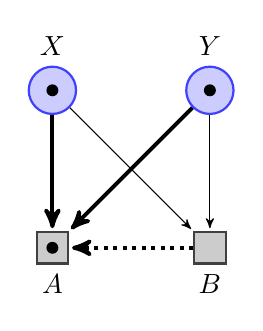
\begin{tikzpicture}[node distance=2cm,>=stealth',bend angle=45,auto]

  \tikzstyle{place}=[circle,thick,draw=blue!75,fill=blue!20,minimum size=6mm]
  \tikzstyle{transition}=[rectangle,thick,draw=black!75,
  			  fill=black!20,minimum size=4mm]

  \tikzstyle{every label}=[black]

  \begin{scope}
    % First net
    \node [place,tokens=1]                  (r1) [label=above:$X$]             {};
    \node [place,tokens=1]                  (r2) [right of=r1,label=above:$Y$] {};
    \node [transition,tokens=1]             (p1) [below of=r1,label=below:$A$] {}
      edge [pre, line width=0.5mm]          (r1)
      edge [pre, line width=0.5mm]          (r2);
    \node [transition]                      (p2) [below of=r2,label=below:$B$] {}
      edge [pre]                            (r1)
      edge [pre]                            (r2)
      edge [post, dotted, line width=0.5mm] (p1);
   \end{scope}
\end{tikzpicture}
\end{center}
\caption{Bi-fan network with additional inhibition element, dots indicate variables captured in model}
\label{bifan_syn}
\end{figure}

\subsubsection{Quantifying redundancy}
%DIF <  SHOULD I RESERVE I_red FOR REDUNDANCY IN GENERAL?
%DIF <  SHOULD I USE \mathcal{R}?
%DIF >  Conclusion ought to be "not good enough" because they cannot be solved analytically

The \DIFdelbegin \DIFdel{question is how to quantify }\DIFdelend \DIFaddbegin \DIFadd{problem of creating a PID can be solved by quantifying }\DIFaddend either the synergetic information \DIFdelbegin \DIFdel{, }\DIFdelend or the redundant information; once one is found, the other follows.
\DIFdelbegin \DIFdel{Some }\DIFdelend \DIFaddbegin \DIFadd{Several }\DIFaddend quantifications have been proposed \DIFdelbegin \DIFdel{, such as the relatively simple redundancy }\DIFdelend \DIFaddbegin \DIFadd{over the years.
An early attempt at a redundancy quantification was the }\DIFaddend measure
%
\begin{equation}
\mathrm{I}_\mathrm{red} = \sum_{j=1}^n [\mathrm{I}\DIFdelbegin \DIFdel{^\mathrm{P}(}\DIFdelend \DIFaddbegin \left( \DIFaddend X_j\DIFaddbegin \DIFadd{^k}\DIFaddend ;Y \DIFdelbegin \DIFdel{)}\DIFdelend \DIFaddbegin \right) \DIFaddend ] - \mathrm{I} \DIFdelbegin \DIFdel{^\mathrm{P}(}\DIFdelend \DIFaddbegin \left( \DIFaddend X;Y \DIFdelbegin \DIFdel{)
}\DIFdelend \DIFaddbegin \right)
\DIFaddend \end{equation}
%
where $\mathrm{I}^\mathrm{P}(X;Y)$ represents the mutual information between $X$ and $Y$\DIFdelbegin \DIFdel{after $X$ has been injected with a fixed amount of random noise, to turn the static system into a system of dependent PDFs \mbox{%DIFAUXCMD
\cite{tononi1999measures}}%DIFAUXCMD
.
This quantifications measures whether the sum of the mutual information measures between the elements of $X$ with $Y$ is higher than the total mutual information between $X$ and $Y$, annd is paired with a degeneracy quantification by the author, designed to measure if the mutual information between increasingly large subsets of $X$ }\DIFdelend \DIFaddbegin \DIFadd{, $X_j^k$ the $j$-th subset of the set $\mathbf{X}$ of size $k$, }\DIFaddend and \DIFdelbegin \DIFdel{$Y$ scales linearly with }\DIFdelend \DIFaddbegin \DIFadd{$n$ the number of possible subsets of size $k$ \mbox{%DIFAUXCMD
\cite{tononi1999measures}}%DIFAUXCMD
}\footnote{\DIFadd{In this study redundancy in causal relations was examined, so the MI was computed over an injection of random noise into the system.}}\DIFadd{.
This quantification is based on the same principle as the WMS-synergy (discussed in the next section), and was predated by the first use of this measure \mbox{%DIFAUXCMD
\cite{gawne1993independent}}%DIFAUXCMD
.
This measure overestimates redundancy, as it will count information shared by $n_\mathrm{shared}$ variables $n_\mathrm{shared}$ times.
The author uses this measure to create a profile of a system by gradually increasing }\DIFaddend the subset size \DIFaddbegin \DIFadd{$k$}\DIFaddend .

% Then minimal information
A more recent proposal is the minimal information $\mathrm{I}_\mathrm{min}$ \cite{williams2010nonnegative}.
This is defined as
%
\begin{equation}
\mathrm{I}_\mathrm{min} \DIFdelbegin \DIFdel{(}\DIFdelend \DIFaddbegin \left( \DIFaddend Y;{X_1, X_2,...,X_k} \DIFdelbegin \DIFdel{) }\DIFdelend \DIFaddbegin \right) \DIFaddend = \sum_s [\DIFdelbegin \DIFdel{p(}\DIFdelend \DIFaddbegin \DIFadd{\Pr }\left( \DIFaddend s \DIFdelbegin \DIFdel{) }\DIFdelend \DIFaddbegin \right) \DIFaddend \min_{X_i} [\mathrm{I}\DIFdelbegin \DIFdel{(}\DIFdelend \DIFaddbegin \left( \DIFaddend Y=y;X_i \DIFdelbegin \DIFdel{)}\DIFdelend \DIFaddbegin \right)\DIFaddend ]]
\end{equation}
%
where \DIFdelbegin \DIFdel{$\mathrm{I}(Y = y;X)$ }\DIFdelend \DIFaddbegin \DIFadd{$\mathrm{I}\left( Y = y;X \right)$ }\DIFaddend is the specific information.
This quantifies information related to a specific outcome, and can be reduced through summation (or integration in the continuous case) over $y$ to the mutual information.
In more recent years, this was still cited as the best redundancy measure, although it has its flaws and should be used with discretion \cite{lizier2013towards, olbrich2015information}.

% Finally bivariate redundancy
Critics of the minimal informtion have proposed an alternative based on PDF projections \cite{harder2013bivariate}.
This quantification meets all requirements \DIFaddbegin \DIFadd{for redundancy }\DIFaddend posed by Williams and Beer, and meets an additional criterium that Harder et al. proposed.
The bivariate redundancy is expressed as
%
\begin{equation}
\mathrm{I}_\mathrm{biv} \DIFdelbegin \DIFdel{(}\DIFdelend \DIFaddbegin \left( \DIFaddend Y;{X_1, X_2} \DIFdelbegin \DIFdel{) }\DIFdelend \DIFaddbegin \right) \DIFaddend = \min [\mathrm{I}_Z^\pi \DIFdelbegin \DIFdel{(}\DIFdelend \DIFaddbegin \left( \DIFaddend X\DIFaddbegin \DIFadd{_1 }\DIFaddend \searrow \DIFdelbegin \DIFdel{Y)}\DIFdelend \DIFaddbegin \DIFadd{X_2 }\right)\DIFaddend , \mathrm{I}_Z^\pi \DIFdelbegin \DIFdel{(Y }\DIFdelend \DIFaddbegin \left( \DIFadd{X_2 }\DIFaddend \searrow X\DIFdelbegin \DIFdel{)}\DIFdelend \DIFaddbegin \DIFadd{_1 }\right)\DIFaddend ] 
\end{equation}
%
where \DIFdelbegin \DIFdel{$\mathrm{I}_Z^\pi (Y \searrow X)$ }\DIFdelend \DIFaddbegin \DIFadd{$\mathrm{I}_Z^\pi \left( X_1 \searrow X_2 \right)$ }\DIFaddend is the projected information of \DIFdelbegin \DIFdel{$Y$ on $X$, defined through }\DIFdelend \DIFaddbegin \DIFadd{$X_1$ on $X_2$.
This projected information is based on the minimization of }\DIFaddend the Kullback-Leibler divergence \DIFdelbegin \DIFdel{as
%DIF < 
}\begin{displaymath}
\DIFdel{\mathrm{I}_Z^\pi (X \searrow Y) = \sum_x p(x) }[\DIFdel{D_\mathrm{KL} (p(z|x) \| p(z)) - D_\mathrm{KL} (p_{(x \searrow Y)}(z|x) \| p(z))}]
\end{displaymath}
%DIFAUXCMD
\DIFdelend \DIFaddbegin \DIFadd{over the space of all probability distributions over $Y$.
As such, this measure cannot be solved analytically and requires numerical optimization.
This attaches a significant computational cost to any redundancy estimation.
It is also difficult to extend, as it is designed for a scenario with 3 variables. %DIF >  As such, we don't go into more detail...
}\DIFaddend 

\subsubsection{Quantifying synergy}
%DIF <  SYNERGY: from old to new, see OLBRICH 2015 and GRIFFITH 2014
%DIF >  From old to new, see Olbrich 2015 and Griffith 2014

%DIF >  Which requirements should be obeyed
For synergy, a number of measures have been proposed as well \cite{griffith2014quantifying, olbrich2015information}.
\DIFaddbegin \DIFadd{A good measure for synergy should meet several criteria, according to \mbox{%DIFAUXCMD
\cite{griffith2014quantifying}}%DIFAUXCMD
.
All in all, we would like the following properties for a synergy measure:
%DIF > 
} \begin{itemize} 
\item \DIFadd{Must fall in the range $0 \le \mathrm{I}_\mathrm{syn}\left( X;Y \right) \le \mathrm{I} \left( X;Y \right)$ (correct range)
}\item \DIFadd{Is invariant to duplicate predictors (resilience)
}\item \DIFadd{Should not systematically under- or overestimate synergy (accuracy)
}\item \DIFadd{Not resource-intensive to compute (computational cost)
} \end{itemize} 
%DIF > 
\DIFadd{At this moment there is no synergy measure that meets all these requirements.
The weight of each individual requirement is dependent on the type of research; for instance, a study reliant on repeated synergy computations favors easy-to-compute quantifiers.
}

\DIFaddend An early synergy measure is the $\mathrm{I}_\mathrm{max}$-synergy, denoted $\mathcal{S}_\mathrm{max}$ \cite{williams2010nonnegative}.
This quantity is closely related to the redundancy measure
%
\begin{equation}
\mathrm{I}_\mathrm{max} \DIFdelbegin \DIFdel{(X}\DIFdelend \DIFaddbegin \left( \DIFadd{\mathbf{X}}\DIFaddend ;Y \DIFdelbegin \DIFdel{) = \sum_{y \in Y} }%DIFDELCMD < [ %%%
\DIFdel{p(Y }\DIFdelend \DIFaddbegin \right) \DIFaddend = \DIFdelbegin \DIFdel{y) }\DIFdelend \max_i \DIFaddbegin [\DIFaddend \mathrm{I} \DIFdelbegin \DIFdel{(}\DIFdelend \DIFaddbegin \left( \DIFaddend X\DIFdelbegin \DIFdel{_i }\DIFdelend \DIFaddbegin \DIFadd{_{i}}\DIFaddend ;Y \DIFdelbegin \DIFdel{= y) }\DIFdelend \DIFaddbegin \right)\DIFaddend ]
\end{equation}
%
\DIFdelbegin \DIFdel{and is }\DIFdelend \DIFaddbegin \DIFadd{as it has the property
%DIF > 
}\begin{equation}
\DIFadd{\mathcal{S}_\mathrm{max} \left( \mathbf{X};Y \right) \equiv \mathrm{I} \left( \mathbf{X};Y \right) - \mathrm{I}_\mathrm{max} \left( \mathbf{X};Y \right)
}\end{equation}
%DIF > 
\DIFadd{The $\mathrm{I}_\mathrm{max}$-synergy measure is formally }\DIFaddend defined as
%
\begin{equation}
\mathcal{S}_\mathrm{max} \DIFdelbegin \DIFdel{(X}\DIFdelend \DIFaddbegin \left( \DIFadd{\mathbf{X}}\DIFaddend ;Y \DIFdelbegin \DIFdel{) }\DIFdelend \DIFaddbegin \right) \DIFaddend = \mathrm{I} \DIFdelbegin \DIFdel{(X}\DIFdelend \DIFaddbegin \left( \DIFadd{\mathbf{X}}\DIFaddend ;Y \DIFdelbegin \DIFdel{) }\DIFdelend \DIFaddbegin \right) \DIFaddend - \DIFaddbegin \DIFadd{\sum_{y \in Y} }[ \DIFadd{\Pr }\left( \DIFadd{Y = y }\right) \DIFadd{\max_i }\DIFaddend \mathrm{I} \DIFdelbegin \DIFdel{_\mathrm{max} (}\DIFdelend \DIFaddbegin \left( \DIFaddend X\DIFaddbegin \DIFadd{_i }\DIFaddend ; Y \DIFdelbegin \DIFdel{)
}\DIFdelend \DIFaddbegin \DIFadd{= y }\right) ]
\DIFaddend \end{equation}
%
\DIFaddbegin \DIFadd{where $\mathrm{I} \left( X_i ; Y = y \right)$ is called the "specific-surprise".
The usage of the specific-surprise makes this measure difficult to apply to systems where we have a set of predicted variables $\mathbf{Y}$.
}\DIFaddend This measure per definition obeys the axiom in \DIFdelbegin \DIFdel{equation~\ref{red_plus_syn_is_mi}}\DIFdelend \DIFaddbegin \DIFadd{Eq.~\ref{red_plus_syn_is_mi}, as we define the synergy as the difference between the mutual information (the non-unique information) and the redundancy }\DIFaddend \cite{griffith2014quantifying}.
It is \DIFdelbegin \DIFdel{said to typically overestimate synergy, and can thus function as an upper bound of sorts}\DIFdelend \DIFaddbegin \DIFadd{resilient against duplicate predicotrs, has a low computational cost, and falls in the correct range.
However, this measure does overestimate synergy as it qualifies unique information as synergy when multiple predictors have unique information on the target}\DIFaddend .

% LOWER BOUND IS NICE TO IMPLEMENT REGARDLESS, EASY TO DO
A second measure is the whole-minus-sum (WMS) synergy, a signed measure where a positive value
signifies synergy \DIFaddbegin \DIFadd{\mbox{%DIFAUXCMD
\cite{gawne1993independent, griffith2014quantifying}}%DIFAUXCMD
}\DIFaddend .
This can be expressed as
%
\begin{equation}
\mathrm{WMS} \DIFdelbegin \DIFdel{(}\DIFdelend \DIFaddbegin \left( \DIFaddend X;Y \DIFdelbegin \DIFdel{) }\DIFdelend \DIFaddbegin \right) \DIFaddend = \mathrm{I} \DIFdelbegin \DIFdel{(}\DIFdelend \DIFaddbegin \left( \DIFaddend X;Y \DIFdelbegin \DIFdel{) }\DIFdelend \DIFaddbegin \right) \DIFaddend - \sum_i [\mathrm{I} \DIFdelbegin \DIFdel{(}\DIFdelend \DIFaddbegin \left( \DIFaddend X_i;Y \DIFdelbegin \DIFdel{)}\DIFdelend \DIFaddbegin \right)\DIFaddend ]
\label{WMS}
\end{equation}
%
\DIFdelbegin \DIFdel{As this is essentially the synergyminus the redundancy , the }\DIFdelend \DIFaddbegin \DIFadd{This measure underestimates synergy, as it subtracts redundancy shared by $n$ variables $n$ times instead of once.
This underestimation becomes worse once systems become larger, as redundancy can be shared by more variables.
It is cheap to compute, but does not always fall in the preferred range.
The }\DIFaddend WMS-synergy can be used a lower bound for the synergy in a system \cite{griffith2014quantifying, olbrich2015information}.

For the bivariate case, the synergy from unique information can be used, $\mathcal{S}_\mathrm{vk}$ \cite{bertschinger2014quantifying, griffith2014quantifying, olbrich2015information}.
This is expressed as
\begin{equation}
\mathcal{S}_\mathrm{vk} \DIFdelbegin \DIFdel{(}\DIFdelend \DIFaddbegin \left( \DIFaddend X;Y \DIFdelbegin \DIFdel{) }\DIFdelend \DIFaddbegin \right) \DIFaddend = \mathrm{I}\DIFdelbegin \DIFdel{(}\DIFdelend \DIFaddbegin \left( \DIFaddend X;Y \DIFdelbegin \DIFdel{) }\DIFdelend \DIFaddbegin \right) \DIFaddend - \mathrm{I}_\mathrm{VK} \DIFdelbegin \DIFdel{(}\DIFdelend \DIFaddbegin \left( \DIFaddend X;Y \DIFdelbegin \DIFdel{)
}\DIFdelend \DIFaddbegin \right)
\DIFaddend \end{equation}
%
where $\mathrm{I}_\mathrm{VK}$ is the \DIFdelbegin \DIFdel{unique information, a measure based on the }\DIFdelend \DIFaddbegin \DIFadd{"union information".
}

\DIFadd{The computation of this union information is a computational process that involves injection of noise into the joint distribution of the entire system, and minimizing a }\DIFaddend Kullback-Leibler \DIFdelbegin \DIFdel{divergence}\DIFdelend \DIFaddbegin \DIFadd{divergence-based measure over the noisified probability distribution.
The idea behind this measure is that synergy is about the whole minus the union of all other predictors, not the whole minus the sum of all other predictors}\DIFaddend .
This method is cited to be good in the bivariate case, where synergy is measured between $X$ and $Y$ when explaining $Z$ \cite{olbrich2015information}.
\DIFaddbegin \DIFadd{The quantification is a relatively accurate approximation and falls in the desired range, but it is not analytically solvable and computationally expensive to compute.
}\DIFaddend 

% Quax also has his measure
A measure of synergy based on synergistic random variables (SRVs) has also been proposed \cite{quax2017quantifying}.
This method is centered around the determination of a set of SRVs, which have zero mutual information with the individual variables in the inspected system, but a non-zero mutual information with the system as a whole.
The total synergystic information is defined as
\begin{equation}
\label{SRV}
\DIFdelbegin \DIFdel{I}\DIFdelend \DIFaddbegin \DIFadd{\mathrm{I}}\DIFaddend _\mathrm{syn}\DIFdelbegin \DIFdel{(}\DIFdelend \DIFaddbegin \left( \DIFaddend X \rightarrow Y\DIFdelbegin \DIFdel{) }\DIFdelend \DIFaddbegin \right) \DIFaddend \equiv \max_k \sum_i \DIFdelbegin \DIFdel{I(}\DIFdelend \DIFaddbegin \DIFadd{\mathrm{I}}\left( \DIFaddend Y \DIFdelbegin \DIFdel{: }\DIFdelend \DIFaddbegin \DIFadd{; }\DIFaddend S_{i,k}^\perp \DIFdelbegin \DIFdel{)
}\DIFdelend \DIFaddbegin \right)
\DIFaddend \end{equation}
where $S_{i,k}$ represents the $i$th SRV in the $k$th set of possible sets of SRVs.
\DIFaddbegin \DIFadd{This measure suffers from a high computational cost, as it involves numerical optimization.
}

%DIF > TODO geef IVK
\DIFaddend 

% IGNORE CORRELATIONAL IMPORTANT, THIS IS NOT A GOOD UPPER BOUND FOR SYNERGY
% SYNERGY FROM MAX ENTROPY ARGUMENTS BECOMES NEGATIVE
Alltogether, this gives us the following summary of the available synergy measures \cite{griffith2014quantifying}:
%
\begin{equation}
\max [0,\mathrm{WMS}\DIFdelbegin \DIFdel{(}\DIFdelend \DIFaddbegin \left( \DIFaddend X;Y \DIFdelbegin \DIFdel{)}\DIFdelend \DIFaddbegin \right)\DIFaddend ] \le \mathcal{S}_\mathrm{VK} \DIFdelbegin \DIFdel{(}\DIFdelend \DIFaddbegin \left( \DIFaddend X;Y \DIFdelbegin \DIFdel{) }\DIFdelend \DIFaddbegin \right) \DIFaddend \le \mathcal{S}\DIFdelbegin \DIFdel{)\mathrm{max} (}\DIFdelend \DIFaddbegin \DIFadd{_\mathrm{max} }\left( \DIFaddend X;Y \DIFdelbegin \DIFdel{) }\DIFdelend \DIFaddbegin \right) \DIFaddend \le \mathrm{I}\DIFdelbegin \DIFdel{(}\DIFdelend \DIFaddbegin \left( \DIFaddend X;Y \DIFdelbegin \DIFdel{)
}\DIFdelend \DIFaddbegin \right)
\DIFaddend \end{equation}
%
\DIFdelbegin \DIFdel{Other notable }\DIFdelend \DIFaddbegin \DIFadd{The more accurate of these measures rely on numerical optimization, and thus require more effort to compute.s
Other notable quantifiers used of }\DIFaddend synergy measures are the correlational importance, which \DIFaddbegin \DIFadd{we do not discuss as it }\DIFaddend was found to \DIFdelbegin \DIFdel{not be a good upper bound for }\DIFdelend \DIFaddbegin \DIFadd{measure something else than }\DIFaddend synergy, and the synergy from maximum entropy arguments, which can take negative values \cite{griffith2014quantifying, olbrich2015information}\DIFaddbegin \DIFadd{.
}\DIFaddend 


\subsection{Complexity Profiles}
\DIFaddbegin \label{sec:profile}
\DIFaddend 



% Why make a profile
As discussed in the previous section, \DIFdelbegin \DIFdel{a complete decomposition of a complex network leads to a }\DIFdelend \DIFaddbegin \DIFadd{we can decompose the information of a system into three categories: synergy, redundancy and unique information.
However, synergy and redundancy can occur at many different levels.
In a 5-predictor system, information could be shared by two variables, but also by five.
Similarly, synergy could emerge from the combination of two variables, or only if all predictors are considered together.
As a result, the }\DIFaddend number of quantifiable relations \DIFdelbegin \DIFdel{that explodes with the }\DIFdelend \DIFaddbegin \DIFadd{explodes with a larger }\DIFaddend system size.
Even when we consider just the \DIFaddbegin \DIFadd{pairwise }\DIFaddend mutual information between all possible subsets of a network, and the output variable, we obtain $2^n$ measurements (including the empty set), an exponential increase.
\DIFdelbegin \DIFdel{Ideally, we compress all }\DIFdelend \DIFaddbegin 

\DIFadd{Due to this rapid increase of the number of quantifiable relations, we would like to extract key characteristics of the system.
For instance, a system might only start showing emergent synergy when considering all predictors together, yet nothing when looking at smaller subsets.
This could be achieved by compressing }\DIFaddend this information in a visual format, that highlights interesting properties of the system as a whole, and disregards unimportant details.
This visualization can take the format of a 'profile' that is characteristic for the type system\DIFdelbegin \DIFdel{, for example a network with synergy at the small scale}\DIFdelend .
When looking at complex systems, the scale is often an important factor regarding complexity, and as such it is often picked as the independent variable in profiles \cite{bar2013computationally, quax2017quantifying, tononi1999measures}.
The \DIFdelbegin \DIFdel{second variable }\DIFdelend \DIFaddbegin \DIFadd{variable on the y-axis }\DIFaddend in the profile shows more variation, and is usually an information theory quantification that is averaged over all subsets of a specified size.

% Talk about early complexity profile
We see the first appearances of complexity profiles regarding biological system in the neurosciences\DIFdelbegin \DIFdel{\mbox{%DIFAUXCMD
\cite{}}%DIFAUXCMD
}\DIFdelend .
It was investigated how redundancy is distributed over the different scales (from subset size 1 to $n$) in simple neural networks \cite{tononi1999measures}.
Several information theory quantifications were proposed as the dependent variable in these profiles, such as
%
 \begin{itemize} 
\item The average MI with the output \DIFdelbegin \DIFdel{$<\mathrm{I}(X^k;Y)>$}\DIFdelend \DIFaddbegin \DIFadd{$<\mathrm{I}\left( X^k;Y \right) >$}\DIFaddend , with $X^k$ being a subset of size $k$
\item The average shared information between the subset, the inverse set, and the output  \DIFdelbegin \DIFdel{$<\mathrm{I}(X^k;X - X^k;Y)>$
}\DIFdelend \DIFaddbegin \DIFadd{$<\mathrm{I}\left( X^k;X - X^k;Y\right) >$
}\DIFaddend \item The average redundancy \DIFdelbegin \DIFdel{$<\mathrm{I}_\mathrm{red}(X;Y)>$
}\DIFdelend \DIFaddbegin \DIFadd{$<\mathrm{I}_\mathrm{red}\left( X;Y\right) >$
}\DIFaddend \item The average system integration \DIFdelbegin \DIFdel{$<\sum_{i = 1}^{\binom{n}{k}}[\mathrm{H}(X^k)] - \mathrm{H}(X)>$
}\DIFdelend \DIFaddbegin \DIFadd{$<\sum_{i = 1}^{\binom{n}{k}}[\mathrm{H}(X^k)] - \mathrm{H}\left( X\right) >$
}\DIFaddend  \end{itemize} 
%
The focus lies strongly on identifying degeneracy or complexity, as \DIFdelbegin \DIFdel{the used definitions }\DIFdelend these quantities can be derived by design through integration of the complexity profile.

%DIF <  Talk about initial profile (short, this has been improved)
\DIFdelbegin \DIFdel{A more advanced complexity profile was conceived by Bar-Yam \mbox{%DIFAUXCMD
\cite{bar2004multiscale}}%DIFAUXCMD
.
The proposed complexity function
%DIF < 
}\begin{displaymath}
\DIFdel{C(k) = \sum_{k^\prime = k}^n D(k^\prime)
}\end{displaymath}
%DIFAUXCMD
%DIF < 
\DIFdel{represents the amount of information shared by at least $k$ variables.
The complexity function utelizes $D(k)$, the information that has a redundancy of $k$ or lower.
This profile has been applied to real-world problems of varying nature in the following years \mbox{%DIFAUXCMD
\cite{bar2013computationally}}%DIFAUXCMD
.
}%DIFDELCMD < 

%DIFDELCMD < %%%
\DIFdelend % Talk about pairwise complexity profile
\DIFdelbegin \DIFdel{As an improvement on his previous proposal, a different }\DIFdelend \DIFaddbegin \DIFadd{An }\DIFaddend approach to a complexity profile is \DIFdelbegin \DIFdel{taken }\DIFdelend \DIFaddbegin \DIFadd{given }\DIFaddend by Bar-Yam \cite{bar2013computationally}.
He constructs a pairwise, non-negative complexity profile based on the mutual information of all variable pairs in the system.
He constructs a function $k_i (p)$ as the number of variables from $x_j \in X$ where $i \ne j$ that have a coupling higher than $p$ with variable $x_i$.
The coupling is defined as a normalized version of the mutual information \DIFdelbegin \DIFdel{$I(x_i;x_j)$}\DIFdelend \DIFaddbegin \DIFadd{$\mathrm{I}\left( x_i;x_j \right)$}\DIFaddend .
This function is inverted to obtain a variable-specific complexity
%DIF < 
%DIF >  NOTE: p is not a probability here!
\begin{equation}
\overset{~}{C}_i\DIFdelbegin \DIFdel{(}\DIFdelend \DIFaddbegin \left( \DIFaddend k \DIFdelbegin \DIFdel{) }\DIFdelend \DIFaddbegin \right)  \DIFaddend = p \DIFdelbegin \DIFdel{(}\DIFdelend \DIFaddbegin \left( \DIFaddend k_i\DIFdelbegin \DIFdel{)
}\DIFdelend \DIFaddbegin \right)
\DIFaddend \end{equation}
%
which is summed and normalized to
%
\begin{equation}
C\DIFdelbegin \DIFdel{(}\DIFdelend \DIFaddbegin \left( \DIFaddend k \DIFdelbegin \DIFdel{) }\DIFdelend \DIFaddbegin \right)  \DIFaddend = \sum_{k^\prime= k}^m \frac{1}{k^\prime} [\overset{~}{C} \DIFdelbegin \DIFdel{(}\DIFdelend \DIFaddbegin \left( \DIFaddend k^\prime \DIFdelbegin \DIFdel{) }\DIFdelend \DIFaddbegin \right) \DIFaddend - \overset{~}{C} \DIFdelbegin \DIFdel{(}\DIFdelend \DIFaddbegin \left( \DIFaddend k^\prime + 1 \DIFdelbegin \DIFdel{)}\DIFdelend \DIFaddbegin \right) \DIFaddend ]
\end{equation}
%
with
%
\begin{equation}
\overset{~}{C} \DIFdelbegin \DIFdel{(}\DIFdelend \DIFaddbegin \left( \DIFaddend k \DIFdelbegin \DIFdel{) }\DIFdelend \DIFaddbegin \right)  \DIFaddend = \sum_{i=1}^n \overset{~}{C}_i \DIFdelbegin \DIFdel{(}\DIFdelend \DIFaddbegin \left( \DIFaddend k \DIFdelbegin \DIFdel{)
}\DIFdelend \DIFaddbegin \right) 
\DIFaddend \end{equation}

As only pairs are examined, this method is computationally a lot cheaper than models that examine all possible subset sizes, costing $\binom{n}{2}$ mutual information computations.
This system is not without downsides\DIFdelbegin \DIFdel{, as fue }\DIFdelend \DIFaddbegin \DIFadd{: due }\DIFaddend to the pairwise nature higher-order relations, such as synergy, are not captured.

% Another option, that is not non-decreasing/increasing
As a response to Bar-Yam's proposal for a complexity function, an alternative that separates structure from entropy has been suggested \cite{arbona2014statistical}.
They provide a complexity function of the form
%
\begin{equation}
C\DIFdelbegin \DIFdel{(}\DIFdelend \DIFaddbegin \left( \DIFaddend s\DIFdelbegin \DIFdel{(}\DIFdelend \DIFaddbegin \left( \DIFaddend \hat{x},t \DIFdelbegin \DIFdel{)) }\DIFdelend \DIFaddbegin \right) \right) \DIFaddend = \mathrm{H}\DIFdelbegin \DIFdel{(}\DIFdelend \DIFaddbegin \left( \DIFaddend s\DIFdelbegin \DIFdel{(}\DIFdelend \DIFaddbegin \left( \DIFaddend \hat{x},t \DIFdelbegin \DIFdel{)) }\DIFdelend \DIFaddbegin \right) \right) \DIFaddend D\DIFdelbegin \DIFdel{(}\DIFdelend \DIFaddbegin \left( \DIFaddend s\DIFdelbegin \DIFdel{(}\DIFdelend \DIFaddbegin \left( \DIFaddend \hat{x},t \DIFdelbegin \DIFdel{))
}\DIFdelend \DIFaddbegin \right) \right)
\DIFaddend \end{equation}
%
where \DIFdelbegin \DIFdel{$D(s(\hat{x},t))$ }\DIFdelend \DIFaddbegin \DIFadd{$D\left( s\left( \hat{x},t \right) \right)$ }\DIFaddend is a correlation measure, and \DIFdelbegin \DIFdel{$s(\hat{x},t)$ }\DIFdelend \DIFaddbegin \DIFadd{$s\left( \hat{x},t \right) $ }\DIFaddend is the state of the system at location $\hat{x}$ and time $t$.
A complexity at time $t$ at a chosen scale level can be derived by integrating this complexity in space.
This complexity measure is especially suitable for spatial information, such as the vector fields relevant in bird flocking behavior.

% Talk about MI profile
%DIF <  Details go in the methods section
%DIF >  Details go in the methods section, here goes only what Rick said to me
It has been suggested by Quax that a mutual information profile such as those proposed by Tononi, where \DIFdelbegin \DIFdel{$< I(X^k;Y) >$ }\DIFdelend \DIFaddbegin \DIFadd{$< \mathrm{I}\left( X^k;Y \right) >$ }\DIFaddend is plotted against the subset size $k$ \DIFdelbegin \DIFdel{\mbox{%DIFAUXCMD
\cite{QuaxPersonal,tononi1999measures}}%DIFAUXCMD
}\DIFdelend \DIFaddbegin \DIFadd{\mbox{%DIFAUXCMD
\cite{QuaxPersonal, tononi1999measures}}%DIFAUXCMD
}\DIFaddend . 
When normalized, this \DIFdelbegin \DIFdel{provides us with }\DIFdelend \DIFaddbegin \DIFadd{would provide }\DIFaddend a non-decreasing, non-negative profile with a range from 0 to 1 \DIFdelbegin \DIFdel{, }\DIFdelend that allows us to detect extreme cases of synergy and redundancy.
If there is no redundancy or synergy, \DIFdelbegin \DIFdel{we expect to see }\DIFdelend a straight line \DIFaddbegin \DIFadd{would form}\DIFaddend .
If the profile is above the straight line, there is more redundancy than synergy in the system, and vice versa if the profile falls below this line, as synergy expresses itself as negative mutual information.
With this information, \DIFaddbegin \DIFadd{Quax argues that }\DIFaddend it is possible to maximum bounds to synergy and redundancy.
For instance, if the profile \DIFdelbegin \DIFdel{instantly }\DIFdelend reaches the maximum possible value \DIFdelbegin \DIFdel{, the is no }\DIFdelend \DIFaddbegin \DIFadd{for a small subset size there cannot be }\DIFaddend synergy in the system.
\DIFdelbegin \DIFdel{If we do not wish to average out the mutual information for each subset size, but instead want to look at the extrems, we can also decide to examine the $\max [ I(X^k;Y) ]$ .
We hope that, in its application, we are able }\DIFdelend \DIFaddbegin \DIFadd{In addition, this can enable one }\DIFaddend to not only attach bounds to synergy and redundancy, but also \DIFaddbegin \DIFadd{observe }\DIFaddend at what subset size-level it occurs.
This can provide valuable information about the way synergy and redundancy are incorporated in the structure of the system.

% Theoretische simpele cases uitwerken
% Belangrijk om een paar voorbeelden uit te werken met MI profielen, laat zien dat een compleet redundant variable een rechte lijn is, maar overlap erboven zit, reken in bits



\subsection{Ecology and Information Theory}
\DIFaddbegin \label{sec:ecology}
\DIFaddend 



\subsubsection{\DIFdelbegin \DIFdel{Paradox of stability }\DIFdelend \DIFaddbegin \DIFadd{Stability }\DIFaddend and complexity \DIFaddbegin \DIFadd{in system biology}\DIFaddend }
% The unanswered question

A major unanswered question in ecology is the relationship between the stability and the \DIFdelbegin \DIFdel{complicatedness of ecosystems.
This problem was posed around the time the field of information theory was founded, in the 1950s, but at the time no answer that was well-supported by emperical data was proposed .
At the time, information theory was immediately picked up as a tool to analyze the complicatedness of ecosystems; the 'evenness variable' $H$, the Shannon-entropy, was used as a measuring device for complicatedness.
The entropy was initially applied on stock measurements, to describe the proportional population sizes of different species in the ecosystem.
}\DIFdelend \DIFaddbegin \DIFadd{complexity of a system \mbox{%DIFAUXCMD
\cite{macarthur1955fluctuations, pimm1977number, kondoh2003foraging}}%DIFAUXCMD
.
Stability is a key factor in the survival of a natural system over longer periods of time.
Some research suggests that natural networks become more stable when they increase in complexity, while others suggest the network become more stable when they are smaller and less densily connected.
Both ideas can be backed by emperical evidence, both from the field and in some cases from computational studies \mbox{%DIFAUXCMD
\cite{chen2001global, kondoh2003foraging}}%DIFAUXCMD
.
As a result, it seems we do not have a full understanding of how complexity interacts with stability, and under what circumstances an increasing complexity in thee system also yields a higher stability.
Understanding what these circumstances are can help us interacting with these systems, for instance in the form of conservation for ecological systems \mbox{%DIFAUXCMD
\cite{kondoh2003foraging}}%DIFAUXCMD
.
This question is not only relevant to predator-prey system, but also in many other biological systems, such as neural networks \mbox{%DIFAUXCMD
\cite{tononi1999measures}}%DIFAUXCMD
.
}\DIFaddend 

\DIFdelbegin \DIFdel{Shortly after, the still popular point of view was formulated that with an increased complicatedness there are more pathways to reach a consumer in the food web, and thus a higher stability.
After all, if one link between prey and predator in a food web would disappear, for instance due to a low preypopulation after a harsh winter, the predator population is relatively unaffected as they switch to a less-preferred yet viable prey }\DIFdelend \DIFaddbegin \DIFadd{On the one hand, it is proposed that larger ecological systems are more stable \mbox{%DIFAUXCMD
\cite{macarthur1955fluctuations}}%DIFAUXCMD
.
Natural systems in many cases take the form of directed graphs, be it a predator-prey network, a neural network, or a gene regulation network.
Nodes in these networks tend to rely on incoming flows, in food webs for intance of energy.
In larger, densily connected systems, a node has more incoming flows.
This reduces the importance of any single edge in the network, making the impact of a single disturbance smaller.
For instance, in a predator-prey network a predator can hunt different types of prey.
Hunting a wider range of species will reduce the impact of a single prey species disappearing.
MacArthur argues that food webs with more links are more stable for this reason, and that this benefit of having as many links as possible is ofset only by a lower trophic efficiency that comes with generalization \mbox{%DIFAUXCMD
\cite{macarthur1955fluctuations}}%DIFAUXCMD
}\DIFaddend .
\DIFdelbegin \DIFdel{When first posed by Macarthur, information theory was used again to form a definition of complicatedness \mbox{%DIFAUXCMD
\cite{macarthur1955fluctuations}}%DIFAUXCMD
,
However, this time, it was used to describe the proportional sizes of biomass flows in }\DIFdelend \DIFaddbegin 

\DIFadd{However, it is also observed that biological networks never appear to have a larger diameter}\footnote{\DIFadd{Disregarding paths between unreachable pairs of nodes, as not in all cases a path can be drawn between a pair of nodes.}} \DIFadd{than 4 or 5 edges \mbox{%DIFAUXCMD
\cite{pimm1977number}}%DIFAUXCMD
.
It was further argued by Pimm et al. that for food webs in particular this is not due to }\DIFaddend the \DIFdelbegin \DIFdel{foodweb, not proportional stocks sizes.
}\DIFdelend \DIFaddbegin \DIFadd{loss of energy over trophic levels, a phenomenom unique to food webs where energy flow only is able to convert 10\% of the energy flowing in into usable energy for the recipient, but due to properties of the network.
Computational studies using models such as the Lotka-Volterra Cascade Models backed this up, suggesting that both an increase in the number of species and a denser connectance between these species decrease the stability of an ecological system \mbox{%DIFAUXCMD
\cite{chen2001global}}%DIFAUXCMD
.
}\DIFaddend 

\DIFdelbegin \DIFdel{Nowadays, the question has solidified itself as a form of paradox.
Theoretical studies generally conclude that smaller systems should be more stable, yet in nature we observe many big an complicated predator-prey networks \mbox{%DIFAUXCMD
\cite{kondoh2003foraging}}%DIFAUXCMD
.
}\DIFdelend The preliminary answers to this question of stability and complicatedness in ecosystems \DIFdelbegin \DIFdel{since then have been }\DIFdelend \DIFaddbegin \DIFadd{in more recent years have remained }\DIFaddend conflicting, especially between emperical \DIFdelbegin \DIFdel{data and theoretical studies . \mbox{%DIFAUXCMD
\cite{pimm1984complexity}}%DIFAUXCMD
.
In the past decade, computational }\DIFdelend studies \DIFdelbegin \DIFdel{have been added to the arsenal of ecologists in their attempt to answer this paradox.
For instance, in a recent computational study the idea of stability through complicatedness due to an increased }\DIFdelend \DIFaddbegin \DIFadd{that observe large networks, and computational studies that favor smaller networks \mbox{%DIFAUXCMD
\cite{pimm1984complexity}}%DIFAUXCMD
.
Attempts have been made to identify a missing element in computational models that can bridge the gap with reality.
An example of such an attempt is the introduction of }\DIFaddend flexibility for predators \DIFdelbegin \DIFdel{has been reinvestigated, and found as a plausible explanation in the ecosystem model \mbox{%DIFAUXCMD
\cite{kondoh2003foraging}}%DIFAUXCMD
.
}\DIFdelend \DIFaddbegin \DIFadd{in predator-prey networks, suggesting that an adapive food choice can preserve stability in larger networks \mbox{%DIFAUXCMD
\cite{kondoh2003foraging}}%DIFAUXCMD
.
However, these attempts are highly problem specific where it might be preferable to look at previously unexplored system properties, such as the presence of synergy. %DIF >  bit cheeky to introduce this, but this is the point why I discuss this
}\DIFaddend 

\subsubsection{\DIFdelbegin \DIFdel{History }\DIFdelend \DIFaddbegin \DIFadd{Use }\DIFaddend of IT in \DIFdelbegin \DIFdel{ecology}\DIFdelend \DIFaddbegin \DIFadd{system biology}\DIFaddend }
% History of IT and biology
%DIF > TODO meer focus per paragraaf, evt elimineer

%DIF >  Key: two different approaches
Information theory has \DIFdelbegin \DIFdel{evidently had a place in ecological research .
%DIF <  Two different approaches
}\DIFdelend \DIFaddbegin \DIFadd{found applications in research into biological systems.
}\DIFaddend However, while ecology does deal with complex systems at many different scales, information theory never took hold as the primary analytical method \cite{ulanowicz2001information}. % Reference to earlier (A)
We can see this manifest itself in the movement away from theoretical studies that involve information theory definitions of complexity to computational studies.
If we look at the applications of information theory in ecology, we see two general approaches to how information theory is applied \cite{ulanowicz2001information}.

%DIF < % METE and Shannon entropy
%DIF > % Shannon entropy
The first application is based on Shannon entropy applied to quasi-static stock numbers.
In this paradigm, complexity is defined through the entropy on the PDF that defines the probability that a random individual pulled from the population is of one species.
In many cases, the amount of biomass is used instead of the number of individuals, as the number of individuals can be a poor representation of the relative presence of a species.
This \DIFaddbegin \DIFadd{method ignores the relationships between species, as edges are not taken into account.
This }\DIFaddend primarily gives us an image of how evenly spread biomass is across all species in an ecosystem, and not necessarily of the complexity of this system.
\DIFdelbegin \DIFdel{While monocultures are often systems of }\DIFdelend \DIFaddbegin \DIFadd{This method does appear to work in some cases; it correctly classifies a monoculture as a system with a }\DIFaddend very low complexity, \DIFdelbegin \DIFdel{systems with a very even speciesdistribution do not have to be.
A food web with few nodes, of which one holds the majority of all biomass, is bound to have a relativily low number of edges, most of which are in contact with the most present species.
A web with many nodes, on the other hand, does not per definition have a large number of edgesand a high connectivity}\DIFdelend \DIFaddbegin \DIFadd{as the system is dominated by a single species.
However, it cannot distinguish between a large system with densily connected species, and an equally large system that has very few edges}\DIFaddend .
As a result, this application of Shannon entropy did not prove very useful to explain complexity \cite{ulanowicz2001information}.
\DIFdelbegin \DIFdel{It is notable that outside of the complexity-resilience question, the Shannon entropy is applied in the process of estimating the geographic distributions of species from limited data \mbox{%DIFAUXCMD
\cite{phillips2006maximum}}%DIFAUXCMD
. %DIF <  maybe throw out
}\DIFdelend 

%% Flows approach
The second movement was reactionary against Shannon, and continued from the work of MacArthur on the complexity-resilience question \cite{ulanowicz2009quantifying}.
Here, the Shannon-entropy is applied on biomass flows, not stock numbers, to determine if all edges in the food web are of similar importance, or if one is vastly more important than the rest.
\DIFaddbegin \DIFadd{This circumenvents the problem that the edges in the system are not considered.
}\DIFaddend In recent years, this concept was elaborated on by Ulanowicz to contrast the efficiency of pathways against the robustness of a predator-prey network \cite{ulanowicz2009quantifying}.
He adds an information theory-based measure for the efficiency of a system, measured \DIFdelbegin \DIFdel{against }\DIFdelend \DIFaddbegin \DIFadd{utilizing }\DIFaddend the conversion rate of energy in a system if all biomass where to travel through the most efficient channels, as well as the reserves, less efficient channels that can pick up slack when more efficient channels fail.
\DIFdelbegin \DIFdel{While looking at the food web gets us a step closer to the stability of an ecosystem, as instabilities tend to cascade through the food web through edges, this is not necessarily a better definition for complexity.
}\DIFdelend In the end, as most ecologists think in stock sizes, not in biomass flows, information theory was written off \DIFaddbegin \DIFadd{\mbox{%DIFAUXCMD
\cite{ulanowicz2001information}}%DIFAUXCMD
}\DIFaddend .

%DIF > % Dyadic
\DIFaddbegin \DIFadd{To the best of our knowledge, dyadic inforation theory principles have only taken hold in neurology.
An analysis using redundancy has suggested that robustness in neural networks is due to degeneracy and redundancy \mbox{%DIFAUXCMD
\cite{tononi1999measures}}%DIFAUXCMD
.
However, this paper is not recent, and uses a definition of redundancy that has fallen out of favor.
We could find few papers discussing a similar topic, although the idea to view in biological complex system in general through redundancy was suggested in a few years after the study by Tononi \mbox{%DIFAUXCMD
\cite{edelman2001degeneracy}}%DIFAUXCMD
.
}

\DIFaddend \subsubsection{Finding synergy in biological complex systems}
% General biology link
% end how we might be able to answer it now

\DIFdelbegin \DIFdel{It has been suggested that synergy in complex systems increases the resilience of this system against nudges \mbox{%DIFAUXCMD
\cite{quax2017quantifying}}%DIFAUXCMD
.
As a result, synergy might be an interesting new approach to the complexity-resilience question.
}\DIFdelend In most previous attempts at using information theory \DIFaddbegin \DIFadd{in system biology}\DIFaddend , it has \DIFaddbegin \DIFadd{either }\DIFaddend been applied on a single ecosystem variable\DIFdelbegin \DIFdel{: the stochastic variable that defines }\DIFdelend \DIFaddbegin \DIFadd{, or for quantifying dyadic interactions.
For instance, the entropy over }\DIFaddend the distribution of biomass or biomass flows within \DIFdelbegin \DIFdel{the ecosystem.
An analysis using redundancy has suggested that robustness is due to degeneracy and redundancy in neural networks.
However, this paper is not recent, and uses a definition of redundancy that has fallen out of favor.
This implies that no analysis is possible that involves interaction between stochastic variables, such as mutual information and synergy .
We propose that we }\DIFdelend \DIFaddbegin \DIFadd{ecosystems has been used as a crude measure for diversity \mbox{%DIFAUXCMD
\cite{ulanowicz2009quantifying}}%DIFAUXCMD
.
Correlations between two genes hae been used in research into the role of genes in disease \mbox{%DIFAUXCMD
\cite{lu2004gene}}%DIFAUXCMD
.
Polyadic relationships are typically not investigated, and only appear in few studies.
}

\DIFadd{It has been suggested that synergy in complex systems increases the resilience of this system against nudges \mbox{%DIFAUXCMD
\cite{quax2017quantifying}}%DIFAUXCMD
.
The concept of synergy also seems to be present on a high level in biological systems; many phenotypical traits we observe in animals are not coded by one gene, but emerge from a set of cooperating genes \mbox{%DIFAUXCMD
\cite{griffith2014quantifying}}%DIFAUXCMD
.
As a result, synergy might be an interesting new approach to the complexity-resilience question.
}

\DIFadd{To look at synergy in biological networks, we need review the manner in which we examine then.
To make a }\DIFaddend shift away from \DIFdelbegin \DIFdel{the }\DIFdelend low-level \DIFdelbegin \DIFdel{information theory principles applied in the past, and start looking at relationships between stochastic variables.
This starts with a reimagination of how we look at an ecosystem.
If }\DIFdelend \DIFaddbegin \DIFadd{quantities, such as entropy, we ought to look at the system as a set of related stochastic variables.
For instance, if }\DIFaddend we do not treat the species of a randomly drawn 'unit' as the random variable \DIFdelbegin \DIFdel{, }\DIFdelend we can consider the population size of each species individually.
\DIFaddbegin 

\DIFadd{As soon as we model the system as a system of dependent random variables, we can start looking at interactions between random variables in order to examine redundancy and synergy in a biological network.
}\DIFaddend This is a very natural step; after all, the disturbances that an ecoystem has to deal with usually manifest itelf as an increase or decrease in the population size of one or several species due to outside forces.
\DIFdelbegin \DIFdel{As soon as we model the system as a system of dependent random variables, we can start looking at interactions between random variables in order to examine redundancy and synergy in a biological network.
}\DIFdelend We can use the time dimension as a way to establish relationships \DIFaddbegin \DIFadd{between }\DIFaddend the state of the system now and later.
This allows us to \DIFdelbegin \DIFdel{use the halflife of effect }\DIFdelend \DIFaddbegin \DIFadd{measure the impact }\DIFaddend of a shock on the \DIFdelbegin \DIFdel{mutual information between the current and }\DIFdelend future state of the system \cite{QuaxPersonal}.
In addition, by simply measuring mutual information between the system now and later we can quantify the amount of memory in a system.
It should be noted that, for this analysis to be performed, time evolution of the system should be possible.
This is the case, for instance, when a \DIFaddbegin \DIFadd{system can be defined using a }\DIFaddend set of ODEs \DIFdelbegin \DIFdel{is defined for the changes in the system over time.
 }%DIFDELCMD < 

%DIFDELCMD <  %%%
\DIFdelend \DIFaddbegin \DIFadd{or a Boolean network.
 }\DIFaddend % Does this fit at all? Reconsider.

\subsection{Complexity and Gene Regulatory Networks}
\DIFaddbegin \label{sec:grn}
\DIFaddend 



\subsubsection{Describing gene regulatory networks}
% Refer to some nice sources for more information on sea urchin and GRN, bolouri is nice for latter, former [2] of kuhn

% The state of network simulation
%% What is a gene regulatory network?
The developmental growth of complex animals is driven by the spatial and temporal activation of gene transcription to mRNA, and consequentially further gene products such as proteins.
This spatial and temporal sequence of states is determined in the genomic regulatory code of an animal \cite{bolouri2002modeling, kuhn2009monte}.
This code specifies gene regulatory networks (GRNs), which are networks of activation- and suppression relationships between genes.
Understanding the GRNs that drive processes in cells is key to understanding how a fertilized egg, a single cell, can grow out to an animal, a large and complex symbiosis of billions of cells.
It can also help us understand the mechanisms behind some human diseases, such as cancer \cite{qian2008inference}.

%% How do we describe gene regulatory networks
Constructing models that capture a GRN accurately is a complicated process.
It is experimentally difficult to measure kinetic \DIFdelbegin \DIFdel{parameteres }\DIFdelend \DIFaddbegin \DIFadd{parameters }\DIFaddend associated with cellular processes in vivo \cite{bolouri2002modeling}.
The most basic way to represent a network is by a full Boolean network \cite{bolouri2002modeling}.
This network maps relationships between genes as instantaneous 'switches', allowing the production of a crude model without in-depth knowledge of reaction rates and delays in the real system.
Boolean networks are constructed through arrayed gene expressions assays, which cluster related genes, followed by a regulatory linkage analysis, which \DIFdelbegin \DIFdel{disruptsthe }\DIFdelend \DIFaddbegin \DIFadd{disrupts the }\DIFaddend activity of a gene to observe the impact on downstream genes in the network \cite{bolouri2002modeling, wu2013high}.

Typically, they are only accurate approximations for small networks \cite{karlebach2008modelling}.
Probabilistic elements can be incorporated in a Boolean network \cite{schlitt2007current}.
This is typically done when empirical data is lacking, and there is uncertainty about the relationships between genes in the network \cite{karlebach2008modelling}.
An extension upon probabilistic Boolean networks is the petrinet, which functions by mimicking the buildup of transcription products over several timesteps \cite{karlebach2008modelling}.
Only when a 'bucket' fills, the down- or upregulation relationship is applied.

%ferrell2011modeling LIST OF MODELS, use this summary and links for dataset, oscillation easy to model in Boolean
Typically, it is ideal to describe a GRN as a mixture of Boolean logic and continuous rules \cite{bolouri2002modeling}.
This is for the reason that Boolean motifs can have vastly different functions based on kinetic properties \cite{ingram2006network}.
They work under strong assumptions, for instance that inhibition dominates over activation\DIFdelbegin \DIFdel{\mbox{%DIFAUXCMD
\cite{}}%DIFAUXCMD
. }\DIFdelend \DIFaddbegin \DIFadd{, which is often the case in real GRN systems \mbox{%DIFAUXCMD
\cite{wang2010process, he2016algorithm}}%DIFAUXCMD
. %DIF >  remove second if published (will remove this anyway I guess)
}\DIFaddend 

Continuous rules are commonly captured in an ODE system or other algebraic formalism that describes the slow reactions involved in activators and surpressors binding to DNA, as well as transcription and translation \cite{ingram2006network}.
An ODE system is typically preferred, as this mimics the reaction dynamics in the cell more closely, but is also more difficult to construct \DIFdelbegin \DIFdel{that }\DIFdelend \DIFaddbegin \DIFadd{than }\DIFaddend a simpler continuous model.
Fast reactions, such as protein-protein interactions, can still be modelled as Boolean switches in these models, as they occur at completely different timescale.
A continuous model can be constructed  from the Boolean counterpart, when additional research is done through the measurement of kinetic data, followed by verification to measure the correspondence of the network with reality \cite{bolouri2002modeling}.
It is preferable to use a non-linear ODE, as GRNs are non-linear in nature \cite{qian2008inference, tyson2003sniffers}.
A proposed improvement upon the common ODE models is that of a sparse additive ODE model, able to capture nonlinear relationships \cite{wu2014sparse}.
Other types of models exist, notably stochastic models, hidden Markov models and \DIFdelbegin \DIFdel{multi-values }\DIFdelend \DIFaddbegin \DIFadd{multi-valued }\DIFaddend Boolean models, but these fall outside the scope of this research \cite{bolouri2002modeling, wu2014sparse}.

The parameters in these models can be notoriously difficult to fit to emperical data, as this requires the search through multi-dimensional space for an optimum fit \cite{bolouri2002modeling, kuhn2009monte}.
This challenge has been tackled with some success using, amongst others, Monte Carlo methods and genetic programming paired with Kalman filtering \cite{qian2008inference, kuhn2009monte}.
More elaborate statistical methods have been developed as well, such as the modified elastic net-method, LASSO-methods and the Bayesian best subset regression \cite{greenfield2013robust, wu2014sparse}.

\subsubsection{Information theory and GRNs}

An inquiry into GRNs using information theory has been made as well, primarily at the level of common network motifs \cite{zhang2012chaotic}.
Positive feedback loops have been found to function as switches and memory units, whereas negative feedback loops have been found to have a noise suppressing or oscilation-inducing function.
Studies have been done into the prevalence of chaotic behavior in GRNs \cite{zhang2012chaotic}.
These resulted in the conclusion that chaotic motifs of size $n\ge 3$ exist, but that they are uncommon in real networks, as they require competition between multiple feedback loops, at least one of which should be a negative feedback loop \cite{zhang2012chaotic}.
In real networks, this condition are scarcely met, although some GRNs do meet this condition, most notably the $n=4$ GRN that regulates the P53-system.

\subsubsection{Available GRN models}

There is a modest selection of GRN models available for further research.
These models are typically released in the SBML-format, an enriched xml-datatype.
\DIFdelbegin %DIFDELCMD < 

%DIFDELCMD < %%%
\DIFdelend One of the best captured and most researched GRNs is the endomesoderm GRN of the sea urchin \cite{bolouri2002modeling, kuhn2009monte}.
This network describes the activity of gene regulation in the early development of the sea urchin embryo, and is still in the proccess of being updated as new studies are done \cite{urchinmodel}.
An \DIFdelbegin \DIFdel{attemt }\DIFdelend \DIFaddbegin \DIFadd{attempt }\DIFaddend has been made to build a full ODE model based on the Boolean abstraction of this GRN using Monte Carlo methods.
This was met with some success, as 65\% of the maximum possible correspondence with emperical data was achieved \cite{kuhn2009monte}.
In this reaction rate-type ODE model, the mRNA concentration linked to a gene (a measure for gene activity) is expressed as
%
\begin{equation}
\frac{dX}{dt} = (\DIFdelbegin \DIFdel{\frac{k_A \cdot A(t)}{c_A + A(t)} }\DIFdelend \DIFaddbegin \DIFadd{\frac{k_A \cdot A\left( t \right)}{c_A + A\left( t \right)} }\DIFaddend + \DIFdelbegin \DIFdel{\frac{k_B \cdot B(t)}{c_B + B(T)}}\DIFdelend \DIFaddbegin \DIFadd{\frac{k_B \cdot B\left( t \right)}{c_B + B\left( t \right)}}\DIFaddend ) \cdot \DIFdelbegin \DIFdel{\frac{k_C \cdot C(t)}{c_C + C(T)} }\DIFdelend \DIFaddbegin \DIFadd{\frac{k_C \cdot C\left( t \right)}{c_C + C\left( t \right)} }\DIFaddend - k_\mathrm{deg} X\DIFdelbegin \DIFdel{(}\DIFdelend \DIFaddbegin \left( \DIFaddend t \DIFdelbegin \DIFdel{)
}\DIFdelend \DIFaddbegin \right)
\DIFaddend \end{equation}
%
where $A$, $B$ and $C$ are protein concentrations, and the lower case letters denote kinetic constants.
Such a model of chemical master equations is popular, like sigmoidal and Michaelis-Menten models, as most limiting processes in gene regulation are chemical reactions \cite{aijo2009learning}.
The model contains of 54 genes, 140 variable species, 278 reactions and 287 parameters.

A model that \DIFdelbegin \DIFdel{mimics }\DIFdelend \DIFaddbegin \DIFadd{puts less focus on mimicking }\DIFaddend real reaction rates \DIFdelbegin \DIFdel{less }\DIFdelend to capture GRNs is a system of continuous non-linear differential equations.
This has been implemented by \cite{qian2008inference} as
%
\begin{equation}
\DIFdelbegin \DIFdel{\frac{dx_i}{dt} }\DIFdelend \DIFaddbegin \DIFadd{\frac{dX_i}{dt} }\DIFaddend = f_i \DIFdelbegin \DIFdel{(x}\DIFdelend \DIFaddbegin \left( \DIFadd{X}\DIFaddend _1,...,\DIFdelbegin \DIFdel{x}\DIFdelend \DIFaddbegin \DIFadd{X}\DIFaddend _n \DIFdelbegin \DIFdel{) }\DIFdelend \DIFaddbegin \right) \DIFaddend + v_i
\end{equation}
%
where
%
\begin{equation}
f_i = \sum_{j=1}^{L_i} [(w_{ij}+ \mu_{ij})\Omega_{ij}\DIFdelbegin \DIFdel{(}\DIFdelend \DIFaddbegin \left( \DIFaddend x_1,...,x_n\DIFdelbegin \DIFdel{)}\DIFdelend \DIFaddbegin \right)\DIFaddend ]
\end{equation}
%
and \DIFdelbegin \DIFdel{$\Omega(x_1,...,x_n)$ }\DIFdelend \DIFaddbegin \DIFadd{$\Omega\left( x_1,...,x_n\right)$ }\DIFaddend is a non-linear function, such as a sigmoid function.
However, no dataset was freely available from this study.

% Yeast model
% Skip the artificial NN for now, we are looking at motifs
Most models, both ODE and Boolean types, have been made \DIFdelbegin \DIFdel{of }\DIFdelend \DIFaddbegin \DIFadd{to describe }\DIFaddend the yeast \textit{S. cerevisiae}, and more recently also \textit{S. pombe} \cite{ferrell2011modeling}. 
As a result, using the \textit{S. cerevisiae} network is encouraged for most purposes, as this network is well validated, up-to-date with current technologies and widely accepted.

% Looking at a subsection
Due to the large size of GRNs, it is often not possible to apply computational methods on the network as a whole.
To circumvent this limitation, \DIFdelbegin \DIFdel{we often look at }\DIFdelend \DIFaddbegin \DIFadd{it is possible to examine functional }\DIFaddend motifs in the network, isolated from the rest.
This can be \DIFdelbegin \DIFdel{donne }\DIFdelend \DIFaddbegin \DIFadd{done }\DIFaddend simply by removing all nodes, save the nodes of interest \cite{zhang2012chaotic}.
When using probability distributions instead of set initial conditions, it is possible to capture the influence of the rest of the network on the input variables \DIFdelbegin \DIFdel{by enforcing correlations between them}\DIFdelend \DIFaddbegin \DIFadd{at the present moment by enforcing emperically determined correlations}\DIFaddend , thus drawing from a joint PDF.
\DIFaddbegin \DIFadd{However, the omitted part of the network is not considered performing an evolution over time.
This implies that isolated motifs should only be examined locally in time. %DIF >  I could phrase this better
}\DIFaddend 


\section{\DIFdelbegin \DIFdel{Methods}\DIFdelend \DIFaddbegin \DIFadd{Methodology}\DIFaddend }
\DIFaddbegin \label{sec:methods}
\DIFaddend 



\subsection{Model design}

\subsubsection{Simulation \DIFdelbegin \DIFdel{Methodology}\DIFdelend \DIFaddbegin \DIFadd{methodology}\DIFaddend }
%DIF > TODO te wollig en te veel informatie: nog steeds na opschonen?
%DIF > TODO last check consistency math notation

% First tell what kind of model we use
As gene regulation is a complicated process of molecular dynamics over time, we are \DIFdelbegin \DIFdel{forced in this type of research to }\DIFdelend represent reality with a \DIFaddbegin \DIFadd{simplified }\DIFaddend model that behaves similarly to reality\DIFdelbegin \DIFdel{, but is less complex}\DIFdelend .
We use a model with both a discrete time-dimension and discrete expression level to describe a gene regulatory system.
A system \DIFdelbegin \DIFdel{contains }\DIFdelend \DIFaddbegin \DIFadd{consists }\DIFaddend of $n$ genes, which can be in state $m \in \{0, 1, ..., l\}$.
The value $l$, the number of possible states, can be configured to be any integer value given $l \ge 2$.
When using $l = 2$, this model reduces to the full Boolean model for gene regulation \cite{bolouri2002modeling}.
Any greater value for $l$ allows for more complex state transistions, and effectively yields us a multi-valued logic model.
\DIFaddbegin 

%DIF >  A reason why we chose this
\DIFaddend We chose this model over an ODE model because of how it provides a naturally constrained sample space.
In \DIFaddbegin \DIFadd{an ODE model, there are a great number of configurable parameters.
For each parameter, only a limited range will be able to produce systems that function remotely like realistic systems.
As these ranges are unknown to us and can take any real value, generating realistic random networks would be a challenge.
In }\DIFaddend this study, sampling random networks is a central part of the experimental design.
A discrete model provides us with a large but finite set, where the size of the sample space is
%
\begin{equation}
|X_\mathrm{total}| = l^{n \cdot l^n}
\end{equation}
%
\DIFdelbegin \DIFdel{The continuous variant, on the other hand, has a large number of configurable parameters that can take on any real value.
As a result, determining a sample space here is much more difficult}\DIFdelend \DIFaddbegin \DIFadd{This makes it easier for us to propose a model that is realistic}\DIFaddend .

% Second, explain the two representations that we use
We use two distinct representations of gene regulation motifs within this framework.
First, we use a transition table form.
This table consists of a mapping from every possible state ($l^n$ in total) to \DIFdelbegin \DIFdel{the }\DIFdelend \DIFaddbegin \DIFadd{its corresponding }\DIFaddend state at $t_\mathrm{next} = t_\mathrm{current} + 1$.
Second, we use a graph form.
In this format, each gene is represented by a node.
Relations between genes are represented as edges between these nodes.
These edges mimics the evolution of the joint PMF over time by functioning as a set of Boolean functions\DIFaddbegin \DIFadd{, which we will refer to as 'rule functions'}\DIFaddend .
These rule \DIFdelbegin \DIFdel{function represent edges in a network motif, which }\DIFdelend \DIFaddbegin \DIFadd{functions }\DIFaddend define the dynamics through which genes regulate each other.
\DIFaddbegin 

%DIF >  A bit more detail into the edges
\DIFaddend Edges have at least one origin and a single target, which map to the in- and outputs of a logic function.
Most of these edges are one-to-one mappings; these are of the type "gene A activates gene B in the next timestep, if A is activated in the current timestep".
Many-to-one mappings are possible; gene A might be translated into a promotor for gene B, but only if the co-enzyme for which gene C codes is also present.
\DIFdelbegin \DIFdel{Many-to-one }\DIFdelend \DIFaddbegin \DIFadd{Many-to-many }\DIFaddend mappings are not included in our model in the framework, as they can be captured by a set of many-to-one relationships, each with the same inputs and a different output.
The possible edges are:
%
 \begin{itemize} 
\item Stimulation (+), adds the expression level $m$ of a single source to the target
\item Inhibition (-), subtracts the expression level $m$ of a single source from the target
\item AND-stimulation, adds the minimum expression level $\min(m_i)$ of all sources to the target
\item AND-inhibition, subtracts the minimum expression level $\min(m_i)$ of all sources from the target
 \end{itemize} 
%
With these edges, this representation mimics the relationships between genes in a natural network.
The AND-variants are designed to mimic co-factors, two gene products that first need to bind to each other before they can simulate or inhibit another gene.
The minimum expression level \DIFdelbegin \DIFdel{is the bottleneck for this expression level}\DIFdelend \DIFaddbegin \DIFadd{of the two inputs is returned}\DIFaddend , as the two gene products only work when formed into a complex.
When a gene is not stimulated, it is assumed that the expression level decays by one every timestep.
It is allowed for in the model for a gene to stimulate itself, which is commonly seen in GRNs \DIFdelbegin \DIFdel{\mbox{%DIFAUXCMD
\cite{}}%DIFAUXCMD
.
}\DIFdelend \DIFaddbegin \DIFadd{\mbox{%DIFAUXCMD
\cite{thomas1995dynamical, zhou2016relative}}%DIFAUXCMD
.
}

%DIF >  Final thoughtss
\DIFaddend A single graph form can correspond to $n!$ different transition tables, depending on how we label the genes in the network.
As all these $n!$ transition tables are in essence the same, we look at all different permutations of the transition table for a single network, and select the top table after sorting.
Now, a graph form always corresponds to a single transition table. 
However, one transition table could \DIFaddbegin \DIFadd{still }\DIFaddend be obtained from several different networks.

\DIFaddbegin \subsubsection{\DIFadd{Time evolution}}

\DIFaddend % Third, explain the time evolution, including the jointpdf
In our study we consider synergetic properties, memory, and resilience of gene regulatory networks.
These properties are measured \DIFdelbegin \DIFdel{on a development of the system }\DIFdelend \DIFaddbegin \DIFadd{as the system develops }\DIFaddend over time.
The distribution of the system over all possible states is defined through a joint probability mass function (PMF), which represents the probability that \DIFdelbegin \DIFdel{a given state of the system occurs}\DIFdelend \DIFaddbegin \DIFadd{the system is found in any state at time $t$}\DIFaddend .
We built upon the implementation of this in the jointPDF-framework \cite{jointpdf}\DIFaddbegin \footnote{\DIFadd{We discuss features that were not used in this study in Appendix~\ref{appendix_methods}.}}\DIFaddend .
In this Python framework, a joint distribution is stored as \DIFdelbegin \DIFdel{a }\DIFdelend \DIFaddbegin \DIFadd{an }\DIFaddend $l$-tree of depth $n$, where $l$ is the number of states a variable can be found in and $n$ is the motif \DIFdelbegin \DIFdel{sized.
The depth of the tree is equal to the sizeof the system}\DIFdelend \DIFaddbegin \DIFadd{size}\DIFaddend .
We can compare two PMFs at two different points in time, each representing a distribution of system states \DIFaddbegin \DIFadd{at that time}\DIFaddend .
As such, we \DIFdelbegin \DIFdel{have consistently use the system $A_{t=0}$ }\DIFdelend \DIFaddbegin \DIFadd{define the system $\mathbf{X}_{t=0}$ }\DIFaddend as the input system, and system \DIFdelbegin \DIFdel{$A_{t=\delta t}$ }\DIFdelend \DIFaddbegin \DIFadd{$\mathbf{X}_{t=\delta t}$ }\DIFaddend as the output system.
Here, $\delta t$ is an step in time in arbitrary units, where we usually \DIFdelbegin \DIFdel{chose }\DIFdelend \DIFaddbegin \DIFadd{choose }\DIFaddend the value $\delta t = 1$. 
The jointPDF-framework supports the generation of a new joint PMF from a starting PMF paired with a transition table.
As a result, we use \DIFdelbegin \DIFdel{the former of our two model definitions }\DIFdelend \DIFaddbegin \DIFadd{a transition table }\DIFaddend for a deterministic time evolution of the distribution of system states.
The result of this is a new $l$-tree describing the joint PMF at time \DIFdelbegin \DIFdel{$t=t_0+dt$}\DIFdelend \DIFaddbegin \DIFadd{$t=t_0+\delta t$}\DIFaddend .

% Turning a network into a transition table
Building a transition table from a network representation \DIFaddbegin \DIFadd{of a GRN motif }\DIFaddend is not trivial.
To find the next state of the system, all rules \DIFaddbegin \DIFadd{functions }\DIFaddend of the motif are applied to the system in the previous state.
If \DIFaddbegin \DIFadd{multiple rules act on the same gene, the outcome is the output that is determined using a 'deciding condition'.
The condition we use, the }\texttt{\DIFadd{totaleffect}}\DIFadd{-condition, sums the outputs of all the functions affecting one gene, with the added condition that the expression level remains within ($0 \le m < l$).
An implication of this is that one strong inhibitor can overpower several weak stimulators completely}\footnote{\DIFadd{All supported deciding conditions are listed in Appendix~\ref{alternative_deciding}}}\DIFadd{.
We build a transition table by determining for each possible state of the system what the next state would be.
It is noted that a self-link is defined to be always active, regardless of its states.
This is commonly done in the literature as well.
If }\DIFaddend there are no rules acting on a gene, it is assumed that its expression level decreases by one due to chemical decay.
A side effect of this is that, while the timesteps are in arbitrary units, the resolution in the time dimension becomes higher with higher-valued logic.
After all, in a Boolean model a gene decays from active to non-active in 1 timestep, whereas in 5-valued logic this will take 5 steps.
\DIFdelbegin \DIFdel{If multiple rules act on the same gene, the outcome is the output that is determined using a 'deciding condition'.
We support four deciding conditions, each of which fit with a different design choice in simplifying reality
%DIF < 
}%DIFDELCMD < \begin{itemize}
 \begin{itemize} %DIFAUXCMD
%DIFDELCMD < \item %%%
\item%DIFAUXCMD
\DIFdel{(}\texttt{\DIFdel{totaleffect}}%DIFAUXCMD
\DIFdel{) Each function affecting a gene outputs a }\textit{\DIFdel{change}} %DIFAUXCMD
\DIFdel{in the target gene, multiple effects are added. The expression level remains capped ($0 \le m \le l$). This implies that one strong inhibitor can overpower several weak stimulators completely.
}%DIFDELCMD < \item %%%
\item%DIFAUXCMD
\DIFdel{(}\texttt{\DIFdel{average}}%DIFAUXCMD
\DIFdel{) Each function affecting a gene outputs a }\textit{\DIFdel{suggested value}} %DIFAUXCMD
\DIFdel{of the target genes , multiple effects combined using a weighted average and rounded to the nearest integer value. This implies that when a gene is both stimulated and inhibited, it is much more likely to end up in a semi-activated state, and not either in a deactivated state or an activated state.
}%DIFDELCMD < \item %%%
\item%DIFAUXCMD
\DIFdel{(}\texttt{\DIFdel{down}}%DIFAUXCMD
\DIFdel{) Each function affecting a gene outputs a }\textit{\DIFdel{suggested value}} %DIFAUXCMD
\DIFdel{of the target genes, the lowest is selected. This method assumes inhibition is dominant.
}%DIFDELCMD < \item %%%
\item%DIFAUXCMD
\DIFdel{(}\texttt{\DIFdel{majority}}%DIFAUXCMD
\DIFdel{) Each function affecting a gene outputs a }\textit{\DIFdel{suggested value}} %DIFAUXCMD
\DIFdel{of the target genes, the most commenly suggested value is chosen. In case of a tie a random value is selected.
}
 \end{itemize} %DIFAUXCMD
%DIFDELCMD < \end{itemize}
%DIFDELCMD < %%%
%DIF < 
\DIFdel{We build a transition table by determining for each state in the current timestep of the transition table, and then for each gene in the state in the next timestep what the expression level is.
It is noted that a self-link is defined to be always active, regardless of its states.
This is commonly done in the literature as well. 
}\DIFdelend \DIFaddbegin 

%DIF >  Limitations of the model
\DIFadd{The size of the set of genes $\mathbf{X}$ entered in the model is in theory arbitrarily big, but in reality limited by computational complexity of the evaluation of the model.
The time evolution of the model runs in $O(l^{c \cdot n})$, as each leaf-value of the $n$-depth tree needs to be evaluated, where $c$ is a constant. 
%DIF >  The WMS syenrgy takes N times MI, MI takes c times entropy, entropy uses marginalize and then does some operations that are probably O(c N
}

\subsubsection{\DIFadd{Initialization of the PDF}}
\DIFaddend 

% Go a bit more into initializing jointPDF
To initialize a jointPDF-object that represents a system \DIFaddbegin \DIFadd{of genes}\DIFaddend , we need to determine an initial distribution of system states.
The \DIFaddbegin \DIFadd{jointPDF }\DIFaddend Python package offers both a uniform and random initialization.
However, in the event that we want to insert a real motif into the model, we added the option to initialize the jointPDF-object in a manner that represents the prevalence of true system states.
For real GRNs, we often have some data about correlations between genes available from empirical studies \DIFdelbegin \DIFdel{\mbox{%DIFAUXCMD
\cite{}}%DIFAUXCMD
}\DIFdelend \DIFaddbegin \DIFadd{\mbox{%DIFAUXCMD
\cite{ideker2001integrated}}%DIFAUXCMD
}\DIFaddend .
For instance, gene \DIFdelbegin \DIFdel{A and gene B }\DIFdelend \DIFaddbegin \DIFadd{$X_0$ and gene $X_1$ }\DIFaddend might rarely be activated together.
Our model can \DIFdelbegin \DIFdel{take }\DIFdelend be configured to use a set of gene-to-gene correlations, \DIFaddbegin \DIFadd{provided in the form of a correlation matrix, }\DIFaddend and base an initial distribution on this.
In this particular scenario, the PMF will be close to zero for all states where gene \DIFdelbegin \DIFdel{A and gene B }\DIFdelend \DIFaddbegin \DIFadd{$X_0$ and gene $X_1$ }\DIFaddend are activated together.

% Explain how to get a PMF from a correlation matrix
Due to the poor scalability of this model, we cannot capture an entire GRN; even in a binary system, the number of leaf-values in the tree structure is $2^k$, where $k$ is the number of genes.
Smaller GRNs contain of around 50 genes typically, which would require a tree too big to process in Python in reasonable time.
To overcome this scaling issue, we isolate a motif from the network.
The rest of the network is inferred through the correlation matrix.
As the correlation matrix is only applied in the first timestep, this model is not suitable for \DIFdelbegin \DIFdel{long simulations }\DIFdelend \DIFaddbegin \DIFadd{simulations of many timesteps}\DIFaddend .

In this study, we focus on generating random networks, with random initial correlations.
The key difference between a joint PMFs with correlations as opposed to a uniform PMF is that the initial entropy is lower; after all, the uncertainty in the distribution is maximized if all states have an equal chance of occuring.
\DIFaddbegin \DIFadd{Real GRN networks are extremely unlikely to have each state be equally likely to occur.
}\DIFaddend As such, the primary goal is to produce initial joint PMFs that are lower in entropy than a uniform distribution\DIFaddbegin \DIFadd{, and are closer in entropy to similar real-world motifs}\DIFaddend . 
For this purpose we do not need a sophisticated model that samples and applies all possible first-order correlations in the network.
We assume a system that can be rewritten as a linear system, where each gene correlates with the previous and the next gene in the system.
As the order of the labels is arbitrary, in practice we assume that our system can be written as a linear system.
This implies that each gene is correlated with at most two other genes, and that there are no correlation loops\DIFaddbegin \footnote{\DIFadd{This is not realistic, but a practical limitation of our model with minimal impact on our results. We discuss this limitation further in section~\ref{sec:discussion}, and discuss future improvements.}}\DIFaddend .

The correlation list is converted to a joint PMF by assuming that the first gene has an equal chance of being in each state.
The result is a tree of depth 1, where each leaf has the same value.
With each subsequent gene that is added, the tree is made one \DIFaddbegin \DIFadd{layer }\DIFaddend deeper.
The ratio in which the probability of each branch is divided over the new leafs is decided by the correlation between the last gene to be added, and the new gene.
\DIFdelbegin \DIFdel{If the in the new leaf both genes are of the same expression level, the }\DIFdelend \DIFaddbegin \DIFadd{The }\DIFaddend new probability is
%
\begin{equation}
\DIFdelbegin \DIFdel{p_\mathrm{leaf} = p}\DIFdelend \DIFaddbegin \label{parentchild}
 \DIFadd{\Pr}\left( \DIFadd{m_\mathrm{child} }\given \DIFadd{m}\DIFaddend _\mathrm{parent} \DIFdelbegin \DIFdel{\cdot (\frac{1}{l} + (1 - \frac{1}{l}) \cdot r)
}\DIFdelend \DIFaddbegin \right) \DIFadd{= 
    }\begin{cases} 
    \Pr(m_\mathrm{parent}) \cdot (\frac{1}{l} + (1 - \frac{1}{l}) \cdot r) &  m_\mathrm{child} = m_\mathrm{parent} \\
    \Pr(m_\mathrm{parent}) \cdot \frac{(1 - (\frac{1}{l} + (1 - \frac{1}{l}) \cdot r))}{l-1} &  m_\mathrm{child} \neq m_\mathrm{parent} \\
    \end{cases}
\DIFaddend \end{equation}
%
where $r$ is the correlation \DIFdelbegin \DIFdel{, and $l$ is the number of expression levels.
The leaf value for a mismatch is then defined as %DIF < 
}\begin{displaymath}
    \DIFdel{p_\mathrm{leaf} = p_\mathrm{parent} \cdot \frac{(1 - (\frac{1}{l} + (1 - \frac{1}{l}) \cdot r))}{l-1} 
}\end{displaymath}
%DIFAUXCMD
%DIF < 
\DIFdelend \DIFaddbegin \DIFadd{between the parent- and child-gene.
The parent gene is the gene with the index preceding the child gene.
The correlation here is simply defined as the percentage chance that the child is in the same state as its parent.
}\DIFaddend This method ensures that the joint PMF remains normalized after each addition, as in the latter equation we simply divide the remaining probability not assigned to the former case equally over the remaining $l-1$ \DIFdelbegin \DIFdel{leafs}\DIFdelend \DIFaddbegin \DIFadd{children}\DIFaddend .

%DIF <  Limitations of the model
\DIFdelbegin \DIFdel{The size of the set $A$ is in theory arbitrarily big, but in reality limited by computational complexity of the evaluation of the model. 
The time evolution of the model runs in $O(l^{c \dot n})$, as each leaf-value of the $n$-depth tree needs to be evaluated.
%DIF <  The WMS syenrgy takes N times MI, MI takes c times entropy, entropy uses marginalize and then does some operations that are probably O(c N)
}%DIFDELCMD < 

%DIFDELCMD < %%%
\subsubsection{\DIFdel{Generating Random State Transitions}}
%DIFAUXCMD
\addtocounter{subsubsection}{-1}%DIFAUXCMD
\DIFdelend \DIFaddbegin \subsubsection{\DIFadd{Generating random state transitions}}
\DIFaddend 

\DIFaddbegin \DIFadd{As a control group, we generate completely random state transitions, representing a completely random system.
}\DIFaddend First, a correlation matrix describing all correlations between the different genes in the motif is randomly generated.
This defines an initial distribution of states for our random motif, and represents the \DIFdelbegin \DIFdel{the }\DIFdelend influence of the part of the GRN that is not part of the motif.
We use a Python implementation of the vine method\DIFdelbegin \DIFdel{\mbox{%DIFAUXCMD
\cite{lewandowski2009generating}}%DIFAUXCMD
.
This method is good for generating }\DIFdelend \DIFaddbegin \DIFadd{, an algorithm to generate }\DIFaddend random correlation matrices with large off-diagonal values \DIFaddbegin \DIFadd{\mbox{%DIFAUXCMD
\cite{lewandowski2009generating}}%DIFAUXCMD
}\DIFaddend .
We then use values on the band above the diagonal as our correlation list\DIFdelbegin \DIFdel{.
}\DIFdelend \DIFaddbegin \DIFadd{, as specified in Eq.~\ref{parentchild}. %DIF > Rick: you mean you consider only corerlations between x and x+1? Not x and x+2? Me: yes, not ideal but good enough given time constraints.
}\DIFaddend 

For the sake of comparison, we sample from the set of all possible transition tables.
\DIFdelbegin \DIFdel{In this process, we consider all the expression levels in }\DIFdelend \DIFaddbegin \DIFadd{We use a completely randomized design}\footnote{\DIFadd{Implementing variance reduction is not impossible, but requires a non-standard design that we will elaborate in section~\ref{sec:discussion}.}}\DIFadd{.
A transition table can be represented by a base-$l$ number, padded with zeroes to the left until it is of length $n \cdot l^n$.
The resulting list of digits represents the expression level of all the genes on the side of our transition table that describes }\DIFaddend the future state of the \DIFdelbegin \DIFdel{transition table as a string of random variables.
For each variable, we sample from the set $m \in \{0, 1, ..., l\}$ with equal probabilities}\DIFdelend \DIFaddbegin \DIFadd{system.
To sample a random number, we draw a random integer for each digit where $0 \le x_\mathrm{random} < l$}\DIFaddend .
As long as the present states are always represented in the same order in the transition table, this allows us to sample any transition table that is possible\DIFdelbegin \DIFdel{with equal probability}\DIFdelend .

\subsubsection{Generating \DIFdelbegin \DIFdel{Biological }\DIFdelend \DIFaddbegin \DIFadd{random biologically realistic }\DIFaddend GRNs}

\DIFaddbegin \DIFadd{We compare the previously generated completely random systems with randomly generated biologically realistic systems.
}\DIFaddend In contrast drawing samples from the set of all possible transition tables, we also want to draw a sample from the sub-samplespace of all biologically possible transition tables.
These should adhere to a set of network properties that are characteristic for GRN motifs, as well as be constructable from the stimulation and inhibition rules that exist in GRNs, but should otherwise be completely random.
In order to construct these transition tables, we start by constructing a random GRN in graph form.
This algorithm can be configured by defining a set of possible rules, a number of nodes, a fraction of the edges that should be 1-to-1, and a set of possible indegrees for the motifs.

Again, we start by generating a correlation list.
Then, a list of all possible edges is generated.
We limit many-to-one connections to 2-to-1; any higher number of inputs is hard to explain biologically, as it would require \DIFdelbegin \DIFdel{3 }\DIFdelend \DIFaddbegin \DIFadd{three or more }\DIFaddend gene products to form a complex together.
An edge also is defined to always have only one target, as a many-to-many edge can be rewritten as multiple many-to-one edges.
We do allow self-loops, as these do occur in nature.

With this list, the network generation process is started.
The network is constructed using a scheme related to the Erdős–Rényi algorithm.
A scale-free network (such as a Barabási–Albert network) would have been preferable, but generating one that allows some key characteristics of GRNs is not trivial.
For instance, the Barabási–Albert does not naturally deal with 2-to-1 edges, cannot create cycles in directed graphs, and will not create edges with the same node as the source and target.
An Erdős–Rényi model is a valid choice, as some sources state that this network model applies to gene regulation in some cases in addition to its scale-free counterpart.
In the literature, the Barabási–Albert seems to be a slightly more common choice.
In addition, we argue that the choice does not make a large difference in the results, as our networks are typically so small that there is little difference between the two.

The Erdős–Rényi algorithm from itself is not equipped to deal with 2-to-1 edges.
To solve this problem, we effectively apply the Erdős–Rényi algorithm two times; once for 1-to-1 edges, once for 2-to-1 edges.
Our first step is to determine the desired indegree during each pass.
If we have a $p_\mathrm{1-to-1}$ that describes the desired fraction of 1-to-1 edges, we find that
%
\begin{equation}
k_\mathrm{1-to-1} = k_\mathrm{total} \cdot p_\mathrm{1-to-1}
\end{equation}
%
and
%
\begin{equation}
k_\mathrm{2-to-1} = k_\mathrm{total} \cdot (1 - p_\mathrm{1-to-1})
\end{equation}
%
\DIFaddbegin \DIFadd{given that an edge is either 1-to-1 or 2-to-1 (implying that $p_\mathrm{2-to-1} = 1 -  p_\mathrm{1-to-1}$).
}\DIFaddend From this information, we can calculate the accept probabilities for edges in both the 1-to-1 set, and the 2-to-1 set.
The distribution of the indegree of a node follows a binomial distribution, giving us for both sets the distributions
%
\begin{equation}
\DIFdelbegin \DIFdel{P}\DIFdelend \DIFaddbegin \DIFadd{\Pr}\DIFaddend _\mathrm{1-to-1} \DIFdelbegin \DIFdel{(}\DIFdelend \DIFaddbegin \left( \DIFaddend \mathrm{deg}(v) = k \DIFdelbegin \DIFdel{) }\DIFdelend \DIFaddbegin \right) \DIFaddend = \binom{n}{k} p_\mathrm{1-to-1}^k (1 - p_\mathrm{1-to-1})^{n-k}
\end{equation}
%
and
%
\begin{equation}
\DIFdelbegin \DIFdel{P}\DIFdelend \DIFaddbegin \DIFadd{\Pr}\DIFaddend _\mathrm{2-to-1} \DIFdelbegin \DIFdel{(}\DIFdelend \DIFaddbegin \left( \DIFaddend \mathrm{deg}(v) = k\DIFdelbegin \DIFdel{) }\DIFdelend \DIFaddbegin \right) \DIFaddend = \DIFdelbegin %DIFDELCMD < \binom{n^2}{k} %%%
\DIFdelend \DIFaddbegin \binom{\binom{n}{2}}{k} \DIFaddend p_\mathrm{2-to-1}^k (1 - p_\mathrm{2-to-1})\DIFdelbegin \DIFdel{^{\binom{n}{2}-k}
}\DIFdelend \DIFaddbegin \DIFadd{^{\binom{n}{2} - k}
}\DIFaddend \end{equation}
%
\DIFdelbegin \DIFdel{where we }\DIFdelend \DIFaddbegin \DIFadd{We }\DIFaddend have to keep in mind that we allow self-referring edges\DIFaddbegin \DIFadd{, implying that there are $n$ possible 1-to-1 edges per node.
We do not consider an 2-to-1 edge where both origins are the same as a valid edge, implying here are $n^2 - n$ possible 2-to-1 edges}\DIFaddend .
We can use the mean of a Binomial distribution to calculate the average indegree, which should match the previously calculated average indegrees.
This way, we arrive at the acceptance probabilities of
%
\begin{equation}
p_\mathrm{1-to-1} = \frac{k_\mathrm{1-to-1}}{n}
\end{equation}
%
and
%
\begin{equation}
p_\mathrm{2-to-1} = \frac{k_\mathrm{2-to-1}}{\binom{n}{2}}
\end{equation}
\DIFdelbegin %DIFDELCMD < 

%DIFDELCMD < %%%
\DIFdelend %DIF > 
Having calculated the parameters for the Erdős–Rényi, we execute the algorithm two times; once for 1-to-1 edges, once for 2-to-1 edges.
Once an edge has been selected, a random function is attached to it, such as inhibition or stimulation.

\subsubsection{Parameter \DIFdelbegin \DIFdel{Nudging}\DIFdelend \DIFaddbegin \DIFadd{nudging}\DIFaddend }

%DIF < % Nudging
%DIF >  General nudging
The method of nudging used was based on an implementation by Riesthuis \DIFdelbegin \DIFdel{\ref{DJ_repository}}\DIFdelend \DIFaddbegin \DIFadd{\mbox{%DIFAUXCMD
\cite{DJ_repository}}%DIFAUXCMD
}\DIFaddend .
We pass our motifs, a list of variables that are to be nudged, and a nudge size $0 \le \epsilon \le 1$ that represents the fraction of the total probability that should be moved as part of the nudge.
\DIFdelbegin \DIFdel{We nudge our PDF in such a way }\DIFdelend \DIFaddbegin \DIFadd{The introduce a local nudge, implying }\DIFaddend that the joint \DIFdelbegin \DIFdel{of all non-nudged variables remains unchanged.
For }\DIFdelend \DIFaddbegin \DIFadd{PDF of the variables that are not nudged remains unaltered.
}

%DIF >  How a nudge works
\DIFadd{The nudge is applied as follows.
First, we produce the joint probability matrix $z$ for the }\DIFaddend each possible configuration of our non-nudged variables\DIFdelbegin \DIFdel{, we produce a vector $z$ of probabilities that our system is in the state where our nudged variable is holding either of the possible expression levels}\DIFdelend .
For instance, \DIFaddbegin \DIFadd{if we apply a nudge on the gene $X_0$ }\DIFaddend in a system \DIFdelbegin \DIFdel{of }\DIFdelend \DIFaddbegin \DIFadd{with }\DIFaddend $n=2$ and $l=2$\DIFaddbegin \DIFadd{, }\DIFaddend we might find $z = [0.2, 0.4]$\DIFdelbegin \DIFdel{if we nudge gene 0, meaning that before the nudge $p_\mathrm{g0 = 0, g1=0} = 0.2$ and $p_\mathrm{g0 = 0, g1=1} = 0.4$}\DIFdelend .
To this \DIFdelbegin \DIFdel{vector }\DIFdelend \DIFaddbegin \DIFadd{matrix }\DIFaddend $z$, a random nudge \DIFdelbegin \DIFdel{vector is applied }\DIFdelend \DIFaddbegin \DIFadd{matrix of the same shape is added }\DIFaddend where the total sum is zero, and the absolute sum being equal to $2 \epsilon \times \sum z$. 
The nudge vector is configured in such a way that \DIFdelbegin \DIFdel{that probabilities should }\DIFdelend \DIFaddbegin \DIFadd{probabilities }\DIFaddend always fall in the range $0 \le p \le 1$ \DIFaddbegin \DIFadd{after the nudge is applied}\DIFaddend .
We do this twice in this example, as \DIFdelbegin \DIFdel{this }\DIFdelend \DIFaddbegin \DIFadd{the }\DIFaddend first only covers the system states where \DIFdelbegin \DIFdel{gene 1 is of the first expression level}\DIFdelend \DIFaddbegin \DIFadd{$m_{X_1} = 0$}\DIFaddend .
The nudged version of the \DIFdelbegin \DIFdel{vector }\DIFdelend \DIFaddbegin \DIFadd{matrix }\DIFaddend $z^\prime$ is plugged back into the jointPDF-object.
\DIFaddbegin 

\DIFaddend In practice, a nudge of \DIFdelbegin \DIFdel{$\epsilon \ge \frac{1}{n}$ or higher }\DIFdelend \DIFaddbegin \DIFadd{$\epsilon \ge \frac{1}{l^{n_\mathrm{nudged}}}$ }\DIFaddend is not safe to use\DIFdelbegin \DIFdel{.
In some cases it will be possible, but if the states are about equally likely this will cause the nudge to not be properly applied, as not enough probability can be moved around.
After all, if we have a simple case of a }\DIFdelend \DIFaddbegin \DIFadd{, where $n_\mathrm{nudged}$ is the number of genes nudged and $l^{n_\mathrm{nudged}}$ is the number of values in $z$.
If we do apply this nudge, it cannot be guaranteed that the nudge can be applied while keeping probabilities in the range $0 \le p \le 1$ after the nudge.
For example, imagine a trivial system with $n = 1$, $l = 2$ and the distribution }\DIFaddend $[0.5, 0.5]$\DIFdelbegin \DIFdel{split, it is impossible to find }\DIFdelend \DIFaddbegin \DIFadd{.
We cannot apply a nudge of $\epsilon = 0.6$, as this would require us to create }\DIFaddend a nudge vector \DIFdelbegin \DIFdel{that we can add to this that satisfies $\epsilon > 0.5$ while also respecting the restraint that probabilities should always fall in the correct range}\DIFdelend \DIFaddbegin \DIFadd{$[0.6, -0.6]$ or $[-0.6, 0.6]$.
Either nudge would leave the system in a state with a negative probability}\DIFaddend .

\subsection{Analytical methods}

\subsubsection{Quantification \DIFdelbegin \DIFdel{Measures}\DIFdelend \DIFaddbegin \DIFadd{measures}\DIFaddend }

% Difference of two joint PDF objects
To measure the effect of parameter nudging on a joint PMF, we use the Hellinger distance to quantify the difference between two distributions.
This is defined as
%
\begin{equation}
\DIFdelbegin \DIFdel{H(}\DIFdelend \DIFaddbegin \DIFadd{\mathrm{H}}\left( \DIFaddend X, Y\DIFdelbegin \DIFdel{) }\DIFdelend \DIFaddbegin \right) \DIFaddend = \frac{1}{\sqrt{2}} \sqrt{\sum^k_{i=1} (\sqrt{x_i} - \sqrt{y_i})^2}
\end{equation}
%
where ${x_1 ... x_k}$ are probabilities of states of $X$ occurring, and ${y_1 ... y_k}$ for states of $Y$.
\DIFaddbegin \DIFadd{We apply the nudge to the system at $t = 0$, and compare the nudged and unnudged system at time $t = \delta t$.
}\DIFaddend When testing the sensitivity to nudges, we always take the average Hellinger distance after applying every possible nudge of the correct 'width'.
For instance, when we apply a nudge on a single target in a system of 4 genes we take the average of 4 values.
This prevents interference of randomness in picking a target gene in our result.
We chose the Hellinger distance \DIFaddbegin \DIFadd{instead }\DIFaddend of the Kullback-Leibler divergence as the latter cannot handle zeros.
Our distributions frequently develop states that have zero probabilities, as GRNs can have unstable states that cannot be reached from any other state.

% Mutual information
\DIFdelbegin \DIFdel{The mutual information is used to inspect information decay over time in the distribution of states in the GRN }\DIFdelend \DIFaddbegin \DIFadd{We quantify the memory of a system using the mutual information $\mathrm{I}\left(\mathbf{X}_t ; \mathbf{X}_{t + \delta t}\right)$.
As no effects are taken into account from outside the system, this also represents the magnitude of causal effects in the }\DIFaddend system.
A mutual information of zero between \DIFdelbegin \DIFdel{the state of the system at $t=0$ and $t=1$ }\DIFdelend \DIFaddbegin \DIFadd{$\mathbf{X}_t$ and $\mathbf{X}_{t + \delta t}$ }\DIFaddend implies that knowledge of the former state provides no insight in the latter.
Similarly, a mutual information equal to the system entropy would imply that everything is known about the system in the latter state when examining the former.
It is implemented as described in Eq.~\ref{MI}, and imported from the jointPDF package \cite{jointpdf}.
We normalize this by dividing by \DIFdelbegin \DIFdel{the entropy of the system at $t = 1$}\DIFdelend \DIFaddbegin \DIFadd{$\mathrm{H}\left(\mathbf{X}_{t + \delta t}\right)$, which yields a measure bounded by zero and one}\DIFaddend .

% Synergy: WMS
% Synergy: Quax
We found that the SRV-based synergy measure proposed by Quax et al. (Eq.~\ref{SRV}) scales poorly with motif size larger than 2 genes \cite{quax2017quantifying}.
As a result we use a simpler synergy measure that is based on the average between an upper- and lower bound estimate for the amount of synergy.
We use the WMS-synergy (Eq.~\ref{WMS}) as a lower bound of synergy in the system.
\DIFaddbegin \DIFadd{This is a computationally cheap measure, and as the systems we measure synergy in are small the intrinsic error in this measure should not be too large.
}\DIFaddend For an upper bound, we use the maximum entropy of a single element of the system and the entropy of the entire system
%
\begin{equation}
\DIFdelbegin \DIFdel{I(X}\DIFdelend \DIFaddbegin \DIFadd{\mathrm{I}}\left( \DIFadd{\mathbf{X}}\DIFaddend _{t=0}; \DIFdelbegin \DIFdel{X_{t=1}) }\DIFdelend \DIFaddbegin \DIFadd{\mathbf{X}_{t=\delta t} }\right) \DIFaddend - \max_i \DIFdelbegin \DIFdel{(I(x}\DIFdelend \DIFaddbegin [\DIFadd{\mathrm{I}}\left( \DIFadd{X}\DIFaddend _{t=0,i};\DIFdelbegin \DIFdel{X_{t=1}))
}\DIFdelend \DIFaddbegin \DIFadd{\mathbf{X}_{t=\delta t}}\right)]
\DIFaddend \end{equation}
%
where $x_i$ is the $i$-th element of the system, and $X$ is the full system.
This \DIFaddbegin \DIFadd{is a variant of the $\mathrm{I}_\mathrm{max}$-synergy described in section~\ref{synergy} which avoids the use of the specific surprise, as this quantity is not readily computed when the set of predicted variables has an arbitrary size.
This }\DIFaddend resembles the WMS-synergy lower bound, but whereas the WMS-synergy assumes that there is no redundancy between the elements in the system, this measure assumes there is full redundancy.
\DIFdelbegin \DIFdel{If there would be full redundancy all the leftover information would be }\DIFdelend \DIFaddbegin \DIFadd{As a result, this measure assumes that all information that does not originate from the system component with the largest MI with the predicted system is }\DIFaddend synergistic in nature, \DIFdelbegin \DIFdel{but if there is no full redundancy the amount synergistic information would be lower, making this a good upper bound }\DIFdelend \DIFaddbegin \DIFadd{creating an upper bound for synergy}\DIFaddend .
The used implementation for the WMS synergy is imported from the jointPDF package \cite{jointpdf}.
We normalize this to fall between 0 and 1 by dividing by \DIFdelbegin \DIFdel{the mutual information between of the system at $t = 0$ and $t = 1$}\DIFdelend \DIFaddbegin \DIFadd{$\mathrm{I}\left( \mathbf{X}_t ; \mathbf{X}_{t + \delta t}\right)$}\DIFaddend .

\subsubsection{Sample \DIFdelbegin \DIFdel{Space Visualization}\DIFdelend \DIFaddbegin \DIFadd{space visualization}\DIFaddend }

An important sanity check is to verify that the sample of biologically possible transition tables shows that this is a subspace of all possible transition tables.
To achieve this, we consider every gene's \DIFdelbegin \DIFdel{state }\DIFdelend \DIFaddbegin \DIFadd{expression level }\DIFaddend in every future state of the transition table as an independent variable.
We then create a 2-dimensional embedding of this vector of random variables using t-Distributed Stochastic Neighbor Embedding (t-SNE), a form of dimensionality reduction that works well on \DIFdelbegin \DIFdel{dataasets }\DIFdelend \DIFaddbegin \DIFadd{datasets }\DIFaddend with many variables per datapoint \cite{maaten2008visualizing}.
\DIFdelbegin \DIFdel{Datapoints }\DIFdelend \DIFaddbegin \DIFadd{All datapoints that are cast in this 2-dimensional embedding }\DIFaddend are colored to indicate whether they are part of the biologically possible set, or the completely random set.
If a portion of the datapoints of one set are clearly not mixing with the other, it is implied that this set covers a part of the sample space that the other does not.
We used a perplexity of 10, which is below the usually recommended value by the Scikit Learn.
This was done as we found that for higher values the datapoints clumped up too much.

\subsubsection{\DIFdelbegin \DIFdel{Searching}\DIFdelend \DIFaddbegin \DIFadd{Cycle finding}\DIFaddend }

\DIFdelbegin \DIFdel{As a validation method, we implemented a search function to explore random samples.
This allows us to search sets of randomly generated motifs for a particular motif of our choosing, for instance one that is common in nature.
This function takes a network-type motif as an input, as well as a set of motifs of any kind.
First, it converts this input motif to a transition table.
Then, all possible variations of the transition table that represent the same motif are produced.
After all, if we switch the labels of two genes in the motif the transition table changes, while the network-motif stays the same.
For each transition table in the sample, we check if it is in the set of transition tables we produced in the previous step.
}%DIFDELCMD < 

%DIFDELCMD < %%%
\subsubsection{\DIFdel{Cycle Finding}}
%DIFAUXCMD
\addtocounter{subsubsection}{-1}%DIFAUXCMD
%DIFDELCMD < 

%DIFDELCMD < %%%
\DIFdel{Cyclicle }\DIFdelend \DIFaddbegin \DIFadd{Cyclical }\DIFaddend sequences of state transitions are a key element of biological networks\DIFdelbegin \DIFdel{. %DIF <  verwijzing naar literatuur eerder
}\DIFdelend \DIFaddbegin \DIFadd{, and can be found in real GRN motifs without considering the rest of the network \mbox{%DIFAUXCMD
\cite{burda2011motifs}}%DIFAUXCMD
.
}\DIFaddend To recognize cycles, we include a cycle-finder in the our framework.
The input for this function is a motif of either type, as well as a maximum cycle length $N_\mathrm{cycle,max}$.
The maximum length, naturally, is limited in theory by the number of possible states.
We work with deterministic systems, so for each state a subsequent state is defined.
As a result, a cycle can at most visit every state once, giving it a length equal to the number of possible states ($N_\mathrm{states} = l^n$).
For each possible initial state we do $N_\mathrm{cycle,max}$ time evaluation.
If we return to the original state, we save this sequence of states as a cycle.
If we encounter a state that is already in a known cycle, we do not return the same cycle twice.
The return value is a list of cycles, each captured in a list of states.
A loop of size 1 is \DIFdelbegin \DIFdel{an }\DIFdelend \DIFaddbegin \DIFadd{a point }\DIFaddend attractor, a larger loop is a \DIFdelbegin \DIFdel{basin of attraction}\DIFdelend \DIFaddbegin \DIFadd{cyclical attractor}\DIFaddend . 

\subsubsection{Complexity \DIFdelbegin \DIFdel{Profile}\DIFdelend \DIFaddbegin \DIFadd{profile}\DIFaddend }

% Introduction to our synergy profile
% Link to introduction
In previous research, the mutual information within a system has been used to investigate complexity in systems of independent and dependent random variables.
A multiple mutual information-based profile has been proposed in the literature that is able to give insights beyond pairwise relations.
A synergy profile can be considered as a plot of the fraction captured of the total mutual information between all input variables and all output variables versus the number of variables taken into consideration, or
%
\begin{equation}
C_\mathrm{mult}(k) = \frac{1}{\binom{n}{k}}\DIFdelbegin \DIFdel{\frac{\sum_{X_i \in [X]^k} [\mathrm{I}(X_i;Y)]}{\mathrm{I}(X;Y)}
}\DIFdelend \DIFaddbegin \DIFadd{\frac{\sum_{X_i \in [\mathbf{X}]^k} [\mathrm{I}\left( X_i;Y \right)]}{\mathrm{I}\left( \mathbf{X};Y\right)}
}\DIFaddend \end{equation}

This profile has the property \DIFdelbegin \DIFdel{$C_\mathrm{mult}(0) = 0$}\DIFdelend \DIFaddbegin \DIFadd{$C_\mathrm{mult}\left( 0 \right) = 0$}\DIFaddend , as for $k = 0$ there is only the empty set, which has zero mutual information with $Y$.
In addition, we know that \DIFdelbegin \DIFdel{$C_\mathrm{mult}(n) = 1$}\DIFdelend \DIFaddbegin \DIFadd{$C_\mathrm{mult}\left( n\right) = 1$}\DIFaddend , as this simply results in
%
\begin{align}
C_\mathrm{mult}\DIFdelbegin \DIFdel{(}\DIFdelend \DIFaddbegin \left( \DIFaddend k \DIFdelbegin \DIFdel{) 
}\DIFdelend \DIFaddbegin \right)  
\DIFaddend &= \frac{1}{\binom{n}{k}}\DIFdelbegin \DIFdel{\frac{\sum_{X_i \in [X]^k} [\mathrm{I}(X_i;Y)]}{\mathrm{I}(X;Y)} }\DIFdelend \DIFaddbegin \DIFadd{\frac{\sum_{X_i \in [\mathbf{X}]^k} [\mathrm{I}\left( X_i;Y\right)]}{\mathrm{I}\left( \mathbf{X};Y\right)} }\DIFaddend \\
&= \DIFdelbegin \DIFdel{\frac{\mathrm{I}(X;Y)}{\mathrm{I}(X;Y)} }\DIFdelend \DIFaddbegin \DIFadd{\frac{\mathrm{I}\left( \mathbf{X};Y\right)}{\mathrm{I}\left( \mathbf{X};Y\right)} }\DIFaddend \\
&= 1
\end{align}

Finally, we can show that this profile is non-decreasing.
We can prove this by imagining an extreme case, where out of variable set $Z$ only $z_1$ provides direct information about the output variable, whereas the rest only provide information when all considered together.
When considering a subset size $1 \le k < n_z $, the complexity will be
%
\begin{equation}
C_\mathrm{mult}\DIFdelbegin \DIFdel{(}\DIFdelend \DIFaddbegin \left( \DIFaddend k \DIFdelbegin \DIFdel{) }\DIFdelend \DIFaddbegin \right)  \DIFaddend = \frac{1}{\binom{k}{n_z}} \mathrm{I}\DIFdelbegin \DIFdel{(}\DIFdelend \DIFaddbegin \left( \DIFaddend z_1;Y\DIFdelbegin \DIFdel{)
}\DIFdelend \DIFaddbegin \right)
\DIFaddend \end{equation}
%
where $n_z$ is the size of set $Z$.
As the mutual information term is constant for $k$, only the fraction determines the complexity value.
As with increasing $k$ fewer and fewer subsets can be made, the function will always be increasing or stagnant, the latter of which is possible only if \DIFdelbegin \DIFdel{$C_\mathrm{mult}(0) = 0$}\DIFdelend \DIFaddbegin \DIFadd{$C_\mathrm{mult}\left( 0 \right) = 0$}\DIFaddend .

As there are many ways to take subsets when $1 < k < n$, we average the sum over all subsets.
However, it is also possible to rewrite this to
%
\begin{equation}
C_\mathrm{mult}\DIFdelbegin \DIFdel{(}\DIFdelend \DIFaddbegin \left( \DIFaddend k \DIFdelbegin \DIFdel{) }\DIFdelend \DIFaddbegin \right) \DIFaddend = \DIFdelbegin \DIFdel{\frac{\max_{X_i \in [X]^k} [\mathrm{I}(X_i;Y)]}{\mathrm{I}(X;Y)}
}\DIFdelend \DIFaddbegin \DIFadd{\frac{\max_{X_i \in [\mathbf{X}]^k} [\mathrm{I}\left( X_i;Y \right)]}{\mathrm{I}\left( \mathbf{X};Y\right)}
}\DIFaddend \end{equation}
%
to focus on extreme values within the set of subsets of size $k$.
In the discrete case, we can simply calculate the mutual information as %DIF < 
\DIFdelbegin \begin{displaymath}
	\DIFdel{I(X;Y) = \sum_{y \in Y} \sum_{x \in X} p(x,y) \log (\frac{p(x,y)}{p(x)p(y)})
}\end{displaymath}
%DIFAUXCMD
%DIF < 
\DIFdel{For a continuous case a complexity profile can be constructed using use k-Nearest Neighbor method described by Kraskov \mbox{%DIFAUXCMD
\cite{kraskov2004estimating}}%DIFAUXCMD
}\DIFdelend \DIFaddbegin \DIFadd{in Eq.~\ref{MI}}\footnote{\DIFadd{For a continuous case a complexity profile can be constructed using use k-Nearest Neighbor method described by Kraskov \mbox{%DIFAUXCMD
\cite{kraskov2004estimating}}%DIFAUXCMD
}}\DIFaddend .

% Subsets
We now can approximate the total mutual information between the input- and the output system.
To produce a plot, we must obtain a mutual information estimate for subsets of each size $1 \le k \le X$, versus the entire output system.
Too obtain this overall estimate for each subset size, we first find the set of mutual informations between every possible subset of $X$ of size $k$, versus the entire system $Y$.
Then, we take the average of the set and divide by the total mutual information between the input- and output system to arrive at the value that corresponds to subset size $k$ in our synergy profile.
We repeat this system for each possible subset size.
Finally, the plot is produced by plotting the $k$ against the corresponding measure.

\subsection{Experimental design}

\subsubsection{Hypotheses}

We hypothesize that:

\DIFdelbegin %DIFDELCMD < \begin{itemize}
%DIFDELCMD < %%%
\DIFdelend \DIFaddbegin  \begin{enumerate} 
\itemsep0em 
\DIFaddend \item There is a \DIFaddbegin \DIFadd{positive }\DIFaddend correlation between synergy and nudge resilience in \DIFdelbegin \DIFdel{network }\DIFdelend \DIFaddbegin \DIFadd{random }\DIFaddend motifs
\item There is a \DIFaddbegin \DIFadd{positive correlation between synergy and nudge resilience in biologically possible motifs
}\item \DIFadd{There is a positive }\DIFaddend correlation between synergy and system memory in \DIFdelbegin \DIFdel{network }\DIFdelend \DIFaddbegin \DIFadd{random motifs
}\item \DIFadd{There is a positive correlation between synergy and system memory in biologically possible }\DIFaddend motifs
\item There is significantly more synergy in a \DIFdelbegin \DIFdel{biological GRN }\DIFdelend \DIFaddbegin \DIFadd{biologically possible }\DIFaddend motif than in a random \DIFdelbegin \DIFdel{GRN }\DIFdelend motif
\item A biologically possible \DIFdelbegin \DIFdel{GRN }\DIFdelend \DIFaddbegin \DIFadd{motif }\DIFaddend scores significantly better in memory than a random \DIFdelbegin \DIFdel{GRN }\DIFdelend motif
\item A biologically possible \DIFdelbegin \DIFdel{GRN }\DIFdelend \DIFaddbegin \DIFadd{motif }\DIFaddend scores significantly better in single-nudge resilience than a random GRN motif
\item A biologically possible GRN does not score significantly differently in multiple-nudge resilience to a random GRN motif
%\item There is a stronger than linear decrease in resilience when increasing the number of variables nudged in a biological GRN motif
\DIFdelbegin %DIFDELCMD < \end{itemize}
%DIFDELCMD < %%%
\DIFdelend \DIFaddbegin  \end{enumerate} 
%DIF >  Rick: dus je hebt eigenlijk wel DRIE populaties van PMFs die je considert, niet slechts twee...? Me: Nee?
\DIFaddend 

To support these \DIFdelbegin \DIFdel{test}\DIFdelend \DIFaddbegin \DIFadd{tests}\DIFaddend , we visualize the \DIFdelbegin \DIFdel{the }\DIFdelend distribution of both biologically possible- and completely random motif in 3D-space, with axes corresponding to the synergy, the system memory, and the system nudge resilience.
We also produce all 2D projections from this 3D distribution of our motifs, three in total, leaving out \DIFdelbegin \DIFdel{on }\DIFdelend \DIFaddbegin \DIFadd{one }\DIFaddend of the three variables in each.
\DIFdelbegin %DIFDELCMD < 

%DIFDELCMD < %%%
\DIFdelend \DIFaddbegin \DIFadd{We calculate both the bivariate correlation and the partial correlation for hypotheses (1)-(4).
}\DIFaddend In addition, we \DIFaddbegin \DIFadd{also produce ensemble of complexity profiles for each experiment, in order to compare the distribution of synergy and redundancy in both random and biologically possible systems.
}

\DIFadd{We }\DIFaddend perform several sanity checks to validate our model.
We check that the biologically feasible motifs are a sub-samplespace through a t-SNE visualization.
We also look at the prevalence of cycles in both samples, as well as how common several real network motifs are in the samples.
In both cases we \DIFdelbegin \DIFdel{expact }\DIFdelend \DIFaddbegin \DIFadd{expect }\DIFaddend a higher rate of occurence in the biologically feasible motifs.
\DIFdelbegin \DIFdel{Finally, we validate our model and measurement methods by running a few transition tables through the model of which we know the expected result.
An example is the X-OR, which should have high synergy and high resilience.
}\DIFdelend \DIFaddbegin \footnote{\DIFadd{We also validated the experimental design by running a few transition tables through the model of which we know the expected result. An example is the X-OR, which should have high synergy and high resilience. This validation is included in the code section of the repository }\url{github.com/dgoldsb/synergy-jointpdf}\DIFadd{.}}
\DIFaddend 

\subsubsection{Parameter ranges}

We perform a parameter sweep over several key parameters.
These parameters could be narrowed down to a range of interest, either due to limits regarding the time complexity of increasing it further, or by using ranges specified in the literature.
The ranges, along with the increments with which we increase in our \DIFdelbegin \DIFdel{sweet}\DIFdelend \DIFaddbegin \DIFadd{sweep}\DIFaddend , are shown in Table~\ref{parameters}.
As part of the experiments all possible numbers of genes targeted by a nudge are evaluated, thus this was excluded from this table.
We decided on an \DIFdelbegin \DIFdel{indegree between 2 and }\DIFdelend \DIFaddbegin \DIFadd{average indegree of }\DIFaddend 4, which seems typical for the smaller GRN networks \cite{lahdesmaki2003learning}.
With this indegree, along with a scale-free design, the random motifs will have similar network properties to actual networks.
Larger networks typically have higher average indegrees, but as Boolean networks are not a good approximation for larger networks this is out of our scope \cite{lahdesmaki2003learning, karlebach2008modelling}.
The nudge size was limited to \DIFdelbegin \DIFdel{below 0.5 units}\DIFdelend \DIFaddbegin \DIFadd{80\% of the maximum safe nudge in the parameter sweep}\DIFaddend , as for higher values the nudging function stopped performing well.
In many cases, the nudged PDF would not remain close to normalized.


\begin{table}
\begin{tabular}{| l | c | c | c |}
\hline
Parameter & Start & End & Increment \\
\hline
Network size (\#) & 2 & 5 & 1 \\
Logic size (\#) & 2 & 5 & 1 \\
Nudge size (fraction of probability) & 0.1 & \DIFdelbeginFL \DIFdelFL{0.5 }\DIFdelendFL \DIFaddbeginFL \DIFaddFL{0.4 }\DIFaddendFL & \DIFdelbeginFL \DIFdelFL{0.1 }\DIFdelendFL \DIFaddbeginFL \DIFaddFL{0.15 }\DIFaddendFL \\
\hline
\end{tabular}
\centering
\caption{The parameter ranges used for the experiments}
\label{parameters}
\end{table}

In addition to these parameter ranges, we \DIFdelbegin \DIFdel{utiluize }\DIFdelend \DIFaddbegin \DIFadd{utilize }\DIFaddend the \texttt{totaleffect} transition function decision rule, and a chance for a 1-to-1 edge of 75\%.
\DIFdelbegin \DIFdel{We pick a random average indegree, which is uniformly distributed between 2 and 4.
}\DIFdelend \DIFaddbegin \DIFadd{This value is chosen as an educated guess, as we did not find a reasonable statistic in the available literature.
}\DIFaddend 


\section{Results}
\DIFaddbegin \label{sec:results}
\DIFaddend 



\subsection{Assumption \DIFdelbegin \DIFdel{Checks}\DIFdelend \DIFaddbegin \DIFadd{checks}\DIFaddend }
%DIF <  TODO: is wilcoxon a Z or W stat?
\DIFaddbegin 

\subsubsection{\DIFadd{Sample space}}
\DIFaddend 

% TSNE
The t-SNE plots do support our assumption that we are sampling only a subspace of all possible systems with our GRN-like random systems.
We show two t-SNE plots in Fig.~\ref{fig:TSNE}, for both a smaller and larger system\footnote{\DIFdelbegin \DIFdel{Additional }\DIFdelend \DIFaddbegin \DIFadd{As it is not possible to include all }\DIFaddend plots \DIFdelbegin \DIFdel{can be found }\DIFdelend \DIFaddbegin \DIFadd{for every experiment in the paper, we make a representative selection, and will make all plots available }\DIFaddend in the repository \url{github.com/dgoldsb/synergy-jointpdf}\DIFaddbegin \DIFadd{.}\DIFaddend }.
\DIFdelbegin \DIFdel{We }\DIFdelend \DIFaddbegin \DIFadd{For larger systems, we }\DIFaddend see a very clear division between the completely random systems (red) and the biologically inspired systems (blue).
\DIFaddbegin \DIFadd{It is important to keep an mind that t-SNE is a dimensionality reduction method that clusters similar datapoints.
As such, the fact that one color does not visibly contain another has no implication on whether one of the two is a subsample.
}\DIFaddend The fact that here and there a random system is mixed in with the biologically inspired system \DIFdelbegin \DIFdel{further indicates }\DIFdelend \DIFaddbegin \DIFadd{does indicate }\DIFaddend that we are dealing with a small subspace; \DIFdelbegin \DIFdel{there is a small chance when sampling from the complete space to draw a system from the subspace}\DIFdelend \DIFaddbegin \DIFadd{it seems possible to sample a biologically possible system when drawing a random system, but not the other way around.
This also suggests that sampling transition tables from biologically possible motifs yields transition tables with similar properties.
For very small systems the sample space is very small, it seems that in this case the biologically possible systems are less easily distinguished from the random systems}\DIFaddend .

\DIFdelbegin %DIFDELCMD < \begin{figure}[H]
%DIFDELCMD <     %%%
\DIFdelendFL \DIFaddbeginFL \begin{figure}[ht]
    \DIFaddendFL \centering
    \begin{subfigure}[b]{0.4\textwidth}
        \DIFdelbeginFL %DIFDELCMD < \includegraphics[width=\textwidth]{./../result_pandas/k=2_l=4/tsne2D.pdf}
%DIFDELCMD <         %%%
\DIFdelendFL \DIFaddbeginFL \includegraphics[width=\textwidth]{./../result_pandas/k=2_l=2/tsne2D.pdf}
        \DIFaddendFL \caption{t-SNE for $k=2$ and $l=4$ (\DIFdelbeginFL \DIFdelFL{$n=900$}\DIFdelendFL \DIFaddbeginFL \DIFaddFL{$n=300$}\DIFaddendFL )}
    \end{subfigure}
    \begin{subfigure}[b]{0.4\textwidth}
        \DIFdelbeginFL %DIFDELCMD < \includegraphics[width=\textwidth]{./../result_pandas/k=4_l=4/tsne2D.pdf}
%DIFDELCMD <         %%%
\DIFdelendFL \DIFaddbeginFL \includegraphics[width=\textwidth]{./../result_pandas/k=5_l=4/tsne2D.pdf}
        \DIFaddendFL \caption{t-SNE for \DIFdelbeginFL \DIFdelFL{$k=4$ }\DIFdelendFL \DIFaddbeginFL \DIFaddFL{$k=5$ }\DIFaddendFL and $l=4$ (\DIFdelbeginFL \DIFdelFL{$n=900$}\DIFdelendFL \DIFaddbeginFL \DIFaddFL{$n=300$}\DIFaddendFL )}
    \end{subfigure}
    \caption{t-SNE plots for varying experiments}
    \label{fig:TSNE}
\end{figure}

\DIFaddbegin \subsubsection{\DIFadd{Transition cycles}}

\DIFaddend % Cycles
We find that biologically inspired systems are much less likely to contain \DIFaddbegin \DIFadd{transition }\DIFaddend cycles than entirely random systems.
In Fig.~\ref{fig:cycles} we show a distribution of the maximum cycle length for a small and large system.
We see that in the smallest systems some small cycles are formed for the GRN-like model.
These cycles, however, disappear once the system size is increased.
\DIFdelbegin \DIFdel{We find that the number of system states $l$ does not have a noticable impact on the cycle distribution in biological systems; we see that cycles become much less likely when increasing the system size, but not when increasing the number of system states. %DIF <  this is weird, because in both cases we increase the number of states
}\DIFdelend As there is always either a cycle or a sink, a maximum cycle length of 1 is the lowest attainable for a system.

\DIFdelbegin %DIFDELCMD < \begin{figure}[H]
%DIFDELCMD <     %%%
\DIFdelendFL \DIFaddbeginFL \begin{figure}[ht]
    \DIFaddendFL \centering
    \begin{subfigure}[b]{0.4\textwidth}
        \includegraphics[width=\textwidth]{./../result_pandas/k=2_l=2/cycles.pdf}
        \caption{Distribution for $k=2$ and $l=2$ (\DIFdelbeginFL \DIFdelFL{$n=900$}\DIFdelendFL \DIFaddbeginFL \DIFaddFL{$n=300$}\DIFaddendFL )}
    \end{subfigure}
    \begin{subfigure}[b]{0.4\textwidth}
        \DIFdelbeginFL %DIFDELCMD < \includegraphics[width=\textwidth]{./../result_pandas/k=3_l=2/cycles.pdf}
%DIFDELCMD <         %%%
\DIFdelendFL \DIFaddbeginFL \includegraphics[width=\textwidth]{./../result_pandas/k=4_l=3/cycles.pdf}
        \DIFaddendFL \caption{Distribution for \DIFdelbeginFL \DIFdelFL{$k=3$ }\DIFdelendFL \DIFaddbeginFL \DIFaddFL{$k=4$ }\DIFaddendFL and \DIFdelbeginFL \DIFdelFL{$l=2$ }\DIFdelendFL \DIFaddbeginFL \DIFaddFL{$l=3$ }\DIFaddendFL (\DIFdelbeginFL \DIFdelFL{$n=900$}\DIFdelendFL \DIFaddbeginFL \DIFaddFL{$n=300$}\DIFaddendFL )}
    \end{subfigure}
    \caption{Histograms of the maximum cycle length distribution}
    \label{fig:cycles}
\end{figure}

% Finding flower motifs, skip for now

\DIFaddbegin \subsubsection{\DIFadd{Normality and outliers}}

\DIFaddend % Normality and all
\DIFaddbegin \DIFadd{To determine if the Pearson test for correlation and the Student's t-test for comparing means were suitable, we check our sample for normality and outliers.
}\DIFaddend In our parameter sweep we drew a large number of separate samples \DIFdelbegin \DIFdel{containting }\DIFdelend \DIFaddbegin \DIFadd{containing }\DIFaddend the synergy, memory, and resilience-properties of networks.
We found that most of these sample \DIFdelbegin \DIFdel{where }\DIFdelend \DIFaddbegin \DIFadd{were }\DIFaddend not normally distributed.
Furthermore, those that did fit a normal distribution often contained outliers, and had wildly varying variances.
As such, we do not meet the assumptions for a t-test for comparing means, and for the Pearson test of correlation.
To handle the sample correctly we use non-parametric statistics in all further analysis, such as the Wilcoxon signed-rank test and the Spearman test of correlation. % these tests throw away the actual values, so outliers  are no problem either, they will simply get the highest/lowest rank

\subsection{Comparisons GRN and Random Systems}

We compared the level of synergy measured in random and biologically inspired systems for varying system sizes and number of states.
We found that completely random systems carry significantly more synergy than the biological systems in all cases.
These results are compiled in Table~\ref{synergy}.

\begin{table}[h]
\begin{tabular}{|c|c|c|c|}
\hline
\diagbox{\# nodes }{\# states}  & 2.0 & 3.0 & 4.0\\
\hline
2.0 & \DIFdelbeginFL \DIFdelFL{37711.00}\DIFdelendFL \DIFaddbeginFL \DIFaddFL{3886.00}\DIFaddendFL *** \cellcolor{yellow!20} & \DIFdelbeginFL \DIFdelFL{35061.00}\DIFdelendFL \DIFaddbeginFL \DIFaddFL{3646.00}\DIFaddendFL *** \cellcolor{yellow!20} & \DIFdelbeginFL \DIFdelFL{36151.00}\DIFdelendFL \DIFaddbeginFL \DIFaddFL{3628.00}\DIFaddendFL *** \cellcolor{yellow!20}\\
\hline
3.0 & \DIFdelbeginFL \DIFdelFL{20577.00}\DIFdelendFL \DIFaddbeginFL \DIFaddFL{2546.00}\DIFaddendFL *** \cellcolor{yellow!20} & \DIFdelbeginFL \DIFdelFL{20246.00}\DIFdelendFL \DIFaddbeginFL \DIFaddFL{2025.00}\DIFaddendFL *** \cellcolor{yellow!20} & \DIFdelbeginFL \DIFdelFL{31266.00}\DIFdelendFL \DIFaddbeginFL \DIFaddFL{3840.00}\DIFaddendFL *** \cellcolor{yellow!20}\\
\hline
4.0 & \DIFdelbeginFL \DIFdelFL{6961.00}\DIFdelendFL \DIFaddbeginFL \DIFaddFL{1151.00}\DIFaddendFL *** \cellcolor{yellow!20} & \DIFdelbeginFL \DIFdelFL{13419.00}\DIFdelendFL \DIFaddbeginFL \DIFaddFL{1118.00}\DIFaddendFL *** \cellcolor{yellow!20} & \DIFdelbeginFL \DIFdelFL{44064.00* }\DIFdelendFL \DIFaddbeginFL \DIFaddFL{4076.00** }\DIFaddendFL \cellcolor{yellow!20}\\
\hline
5.0 & \DIFdelbeginFL \DIFdelFL{1641.00}\DIFdelendFL \DIFaddbeginFL \DIFaddFL{164.00}\DIFaddendFL *** \cellcolor{yellow!20} & \DIFdelbeginFL \DIFdelFL{16660.00}\DIFdelendFL \DIFaddbeginFL \DIFaddFL{1342.00}\DIFaddendFL *** \cellcolor{yellow!20} & \DIFaddbeginFL \DIFaddFL{4613.00* }\cellcolor{yellow!20}\DIFaddendFL \\
\hline
\end{tabular}
\centering
\caption{\DIFdelbeginFL \DIFdelFL{Experiment }\DIFdelendFL \DIFaddbeginFL \DIFaddFL{Comparison of the mean }\DIFaddendFL synergy \DIFdelbeginFL \DIFdelFL{, Z-value }\DIFdelendFL \DIFaddbeginFL \DIFaddFL{between random and biological networks ($n = 100$). Cells contain the $T$-statistic }\DIFaddendFL and significance per experiment (* implies $p<0.05$, ** $p<0.005$, *** $p<0.0005$)\DIFdelbeginFL \DIFdelFL{with n=900. }\DIFdelendFL \DIFaddbeginFL \DIFaddFL{. }\DIFaddendFL Green background implies higher mean in the biological network, yellow higher mean in the random network.}
\label{synergy}
\end{table}

We similarly compared the level of memory measured in random and biologically inspired systems for varying experiments.
We found that completely random systems carry significantly more memory than the biological systems in most cases. % this is to be expected, the memory is really really high
These results are compiled in Table~\ref{memory}\DIFaddbegin \footnote{\DIFadd{The implementation of the Wilcoxon signed-rank test returns a $T$-statistic of zero when the two samples share zero overlap in their range.}}\DIFaddend .

\begin{table}[h]
\begin{tabular}{|c|l|l|l|}
\hline
\diagbox{\# nodes }{\# states}  & 2.0 & 3.0 & 4.0\\
\hline
2.0 & \DIFdelbeginFL \DIFdelFL{27152.00}\DIFdelendFL \DIFaddbeginFL \DIFaddFL{3305.00}\DIFaddendFL *** \cellcolor{yellow!20} & \DIFdelbeginFL \DIFdelFL{1693.00}\DIFdelendFL \DIFaddbeginFL \DIFaddFL{272.00}\DIFaddendFL *** \cellcolor{yellow!20} & \DIFdelbeginFL \DIFdelFL{327.00}\DIFdelendFL \DIFaddbeginFL \DIFaddFL{21.00}\DIFaddendFL *** \cellcolor{yellow!20}\\
\hline
3.0 & \DIFdelbeginFL \DIFdelFL{13465.00}\DIFdelendFL \DIFaddbeginFL \DIFaddFL{1543.00}\DIFaddendFL *** \cellcolor{yellow!20} & \DIFdelbeginFL \DIFdelFL{7.00}\DIFdelendFL \DIFaddbeginFL \DIFaddFL{0.00}\DIFaddendFL *** \cellcolor{yellow!20} & 0.00*** \cellcolor{yellow!20}\\
\hline
4.0 & \DIFdelbeginFL \DIFdelFL{1631.00}\DIFdelendFL \DIFaddbeginFL \DIFaddFL{100.00}\DIFaddendFL *** \cellcolor{yellow!20} & 0.00*** \cellcolor{yellow!20} & 0.00*** \cellcolor{yellow!20}\\
\hline
5.0 & \DIFdelbeginFL \DIFdelFL{17.00}\DIFdelendFL \DIFaddbeginFL \DIFaddFL{0.00}\DIFaddendFL *** \cellcolor{yellow!20} & 0.00*** \cellcolor{yellow!20} & \DIFaddbeginFL \DIFaddFL{0.00*** }\cellcolor{yellow!20}\DIFaddendFL \\
\hline
\end{tabular}
\centering
\caption{\DIFdelbeginFL \DIFdelFL{Experiment }\DIFdelendFL \DIFaddbeginFL \DIFaddFL{Comparison of the mean }\DIFaddendFL memory \DIFdelbeginFL \DIFdelFL{, Z-value }\DIFdelendFL \DIFaddbeginFL \DIFaddFL{between random and biological networks ($n = 100$). Cells contain the $T$-statistic }\DIFaddendFL and significance per experiment (* implies $p<0.05$, ** $p<0.005$, *** $p<0.0005$)\DIFdelbeginFL \DIFdelFL{with n=900. }\DIFdelendFL \DIFaddbeginFL \DIFaddFL{. }\DIFaddendFL Green background implies higher mean in the biological network, yellow higher mean in the random network.}
\label{memory}
\end{table}

We did find a consistent difference in the impact of nudging a single variable.
As shown in Table~\ref{resilience_single}, the nudge impact is higher in random networks.
%Larger system experiments are closer to reality, as gene regulatory networks consist of many genes.
% TODO: mention means

\begin{table}[h]
\begin{tabular}{|l|l|l|l|l|}
\hline
\# nodes & \diagbox{\# states}{$\epsilon$}  & 0.1 & 0.25 & \DIFdelbeginFL \DIFdelFL{0.5}\DIFdelendFL \DIFaddbeginFL \DIFaddFL{0.4}\DIFaddendFL \\
\hline
\multirow{3}{*}{2.0} & 2.0 & \DIFdelbeginFL \DIFdelFL{3102.00*** }\DIFdelendFL \DIFaddbeginFL \DIFaddFL{426.00* }\DIFaddendFL \cellcolor{yellow!20} & \DIFdelbeginFL \DIFdelFL{3671.00*** }\DIFdelendFL \DIFaddbeginFL \DIFaddFL{300.00** }\DIFaddendFL \cellcolor{yellow!20} & \DIFdelbeginFL \DIFdelFL{2753.00}\DIFdelendFL \DIFaddbeginFL \DIFaddFL{285.00}\DIFaddendFL *** \cellcolor{yellow!20}\\
\cline{2-5}
  & 3.0 & \DIFdelbeginFL \DIFdelFL{1182.00}\DIFdelendFL \DIFaddbeginFL \DIFaddFL{152.00}\DIFaddendFL *** \cellcolor{yellow!20} & \DIFdelbeginFL \DIFdelFL{1338.00}\DIFdelendFL \DIFaddbeginFL \DIFaddFL{117.00}\DIFaddendFL *** \cellcolor{yellow!20} & \DIFdelbeginFL \DIFdelFL{763.00}\DIFdelendFL \DIFaddbeginFL \DIFaddFL{92.00}\DIFaddendFL *** \cellcolor{yellow!20}\\
\cline{2-5}
  & 4.0 & \DIFdelbeginFL \DIFdelFL{953.00}\DIFdelendFL \DIFaddbeginFL \DIFaddFL{100.00}\DIFaddendFL *** \cellcolor{yellow!20} & \DIFdelbeginFL \DIFdelFL{609.00}\DIFdelendFL \DIFaddbeginFL \DIFaddFL{59.00}\DIFaddendFL *** \cellcolor{yellow!20} & \DIFdelbeginFL \DIFdelFL{303.00}\DIFdelendFL \DIFaddbeginFL \DIFaddFL{33.00}\DIFaddendFL *** \cellcolor{yellow!20}\\
\cline{2-5}
\hline
\multirow{3}{*}{3.0} & 2.0 & \DIFdelbeginFL \DIFdelFL{1504.00}\DIFdelendFL \DIFaddbeginFL \DIFaddFL{237.00}\DIFaddendFL *** \cellcolor{yellow!20} & \DIFdelbeginFL \DIFdelFL{1420.00}\DIFdelendFL \DIFaddbeginFL \DIFaddFL{173.00}\DIFaddendFL *** \cellcolor{yellow!20} & \DIFdelbeginFL \DIFdelFL{1238.00}\DIFdelendFL \DIFaddbeginFL \DIFaddFL{166.00}\DIFaddendFL *** \cellcolor{yellow!20}\\
\cline{2-5}
  & 3.0 & \DIFdelbeginFL \DIFdelFL{112.00}\DIFdelendFL \DIFaddbeginFL \DIFaddFL{4.00}\DIFaddendFL *** \cellcolor{yellow!20} & \DIFdelbeginFL \DIFdelFL{78.00}\DIFdelendFL \DIFaddbeginFL \DIFaddFL{10.00}\DIFaddendFL *** \cellcolor{yellow!20} & 0.00*** \cellcolor{yellow!20}\\
\cline{2-5}
  & 4.0 & \DIFdelbeginFL \DIFdelFL{5.00}\DIFdelendFL \DIFaddbeginFL \DIFaddFL{0.00}\DIFaddendFL *** \cellcolor{yellow!20} & 0.00*** \cellcolor{yellow!20} & 0.00*** \cellcolor{yellow!20}\\
\cline{2-5}
\hline
\multirow{3}{*}{4.0} & 2.0 & \DIFdelbeginFL \DIFdelFL{391.00}\DIFdelendFL \DIFaddbeginFL \DIFaddFL{68.00}\DIFaddendFL *** \cellcolor{yellow!20} & \DIFdelbeginFL \DIFdelFL{152.00}\DIFdelendFL \DIFaddbeginFL \DIFaddFL{26.00}\DIFaddendFL *** \cellcolor{yellow!20} & \DIFdelbeginFL \DIFdelFL{315.00}\DIFdelendFL \DIFaddbeginFL \DIFaddFL{8.00}\DIFaddendFL *** \cellcolor{yellow!20}\\
\cline{2-5}
  & 3.0 & 0.00*** \cellcolor{yellow!20} & 0.00*** \cellcolor{yellow!20} & 0.00*** \cellcolor{yellow!20}\\
\cline{2-5}
  & 4.0 & 0.00*** \cellcolor{yellow!20} & 0.00*** \cellcolor{yellow!20} & 0.00*** \cellcolor{yellow!20}\\
\cline{2-5}
\hline
\multirow{3}{*}{5.0} & 2.0 & \DIFdelbeginFL \DIFdelFL{6.00}\DIFdelendFL \DIFaddbeginFL \DIFaddFL{0.00}\DIFaddendFL *** \cellcolor{yellow!20} & \DIFdelbeginFL \DIFdelFL{6.00}\DIFdelendFL \DIFaddbeginFL \DIFaddFL{0.00}\DIFaddendFL *** \cellcolor{yellow!20} & \DIFdelbeginFL \DIFdelFL{4.00}\DIFdelendFL \DIFaddbeginFL \DIFaddFL{0.00}\DIFaddendFL *** \cellcolor{yellow!20}\\
\cline{2-5}
  & 3.0 & 0.00*** \cellcolor{yellow!20} & 0.00*** \cellcolor{yellow!20} & 0.00*** \cellcolor{yellow!20}\\
\cline{2-5}
  & 4.0 & \DIFaddbeginFL \DIFaddFL{0.00*** }\cellcolor{yellow!20} \DIFaddendFL & \DIFaddbeginFL \DIFaddFL{0.00*** }\cellcolor{yellow!20} \DIFaddendFL & \DIFaddbeginFL \DIFaddFL{0.00*** }\cellcolor{yellow!20}\DIFaddendFL \\
\cline{2-5}
\hline
\end{tabular}
\centering
\DIFdelbeginFL %DIFDELCMD < \caption{%
{%DIFAUXCMD
\DIFdelFL{Experiment resilience single, Z-value and significance per experiment (* implies $p<0.05$, ** $p<0.005$, *** $p<0.0005$) with n=300. Green background implies higher mean in the biological network, yellow higher mean in the random network.}}
%DIFAUXCMD
\DIFdelendFL \label{resilience_single}
\DIFaddbeginFL \caption{\DIFaddFL{Comparison of the mean nudge impact (a single variable being nudged) between random and biological networks ($n = 100$). Cells contain the $T$-statistic and significance per experiment (* implies $p<0.05$, ** $p<0.005$, *** $p<0.0005$) with n=300. Green background implies higher mean in the biological network, yellow higher mean in the random network.}}
\DIFaddendFL \end{table}

We found a similar consistent difference in the impact of nudging all variables.
As shown in Table~\ref{resilience_multiple} in the appendix, the nudge impact is consistently higher in random networks.
It appears that models with a higher number of states (a higher resolution in the expression level dimension), by virtue of having more expression levels, show a stronger difference in the nudge impact.

In Fig.~\ref{fig:3dscatter} we provide several scatterplots of experiments \DIFdelbegin \DIFdel{, }\DIFdelend \DIFaddbegin \DIFadd{showcasting the distribution of memory, synergy, and resilience for both types of systems }\DIFaddend with varying system sizes and numbers of expression levels\DIFaddbegin \footnote{\DIFadd{2-dimensional versions of these plots are included in Fig.~\ref{fig:2d22}-\ref{fig:2d54} in Appendix~\ref{appendix_figures}}}\DIFaddend .
We find that the variance reduces significantly when increasing the number of possible states, showing a much clearer pattern.
The same effect is seen in when increasing the system size.
This is likely due to the increase in the sample space; the sample space grows strongly when increasing either the system size or number of possible states.
We notice that random systems are very tightly clustered, and typically have an extremely high memory paired with high synergy.
The biological systems are much more spread out, and while there are outliers with higher memory than any random system, most samples have a lower memory and synergy.
The spread of nudge impacts is also much \DIFdelbegin \DIFdel{high }\DIFdelend \DIFaddbegin \DIFadd{higher }\DIFaddend in biological systems than in random systems.

\begin{figure}[H]
    \centering
    \begin{subfigure}[b]{0.45\textwidth}
        \includegraphics[width=\textwidth]{./../result_pandas/k=2_l=2_e=0.250000/scatter3D_memory_synergy_resilience.pdf}
        \caption{Distribution for $k=2$ and $l=2$ (\DIFdelbeginFL \DIFdelFL{$n=900$}\DIFdelendFL \DIFaddbeginFL \DIFaddFL{$n=300$}\DIFaddendFL )}
    \end{subfigure}
    \begin{subfigure}[b]{0.45\textwidth}
        \includegraphics[width=\textwidth]{./../result_pandas/k=2_l=4_e=0.250000/scatter3D_memory_synergy_resilience.pdf}
        \caption{Distribution for $k=2$ and $l=4$ (\DIFdelbeginFL \DIFdelFL{$n=900$}\DIFdelendFL \DIFaddbeginFL \DIFaddFL{$n=300$}\DIFaddendFL )}
    \end{subfigure}
\bigskip
    \begin{subfigure}[b]{0.45\textwidth}
        \DIFdelbeginFL %DIFDELCMD < \includegraphics[width=\textwidth]{./../result_pandas/k=4_l=2_e=0.250000/scatter3D_memory_synergy_resilience.pdf}
%DIFDELCMD <         %%%
\DIFdelendFL \DIFaddbeginFL \includegraphics[width=\textwidth]{./../result_pandas/k=5_l=2_e=0.250000/scatter3D_memory_synergy_resilience.pdf}
        \DIFaddendFL \caption{Distribution for \DIFdelbeginFL \DIFdelFL{$k=4$ }\DIFdelendFL \DIFaddbeginFL \DIFaddFL{$k=5$ }\DIFaddendFL and $l=2$ (\DIFdelbeginFL \DIFdelFL{$n=900$}\DIFdelendFL \DIFaddbeginFL \DIFaddFL{$n=300$}\DIFaddendFL )}
    \end{subfigure}
    \begin{subfigure}[b]{0.45\textwidth}
        \DIFdelbeginFL %DIFDELCMD < \includegraphics[width=\textwidth]{./../result_pandas/k=4_l=4_e=0.250000/scatter3D_memory_synergy_resilience.pdf}
%DIFDELCMD <         %%%
\DIFdelendFL \DIFaddbeginFL \includegraphics[width=\textwidth]{./../result_pandas/k=5_l=4_e=0.250000/scatter3D_memory_synergy_resilience.pdf}
        \DIFaddendFL \caption{Distribution for \DIFdelbeginFL \DIFdelFL{$k=4$ }\DIFdelendFL \DIFaddbeginFL \DIFaddFL{$k=5$ }\DIFaddendFL and $l=4$ (\DIFdelbeginFL \DIFdelFL{$n=900$}\DIFdelendFL \DIFaddbeginFL \DIFaddFL{$n=300$}\DIFaddendFL )}
    \end{subfigure}
    \caption{Scatterplots of synergy, memory and nudge impact (varying $l$ and $k$\DIFaddbeginFL \DIFaddFL{, $\epsilon = 0.25$}\DIFaddendFL )}
    \label{fig:3dscatter}
\end{figure}

\subsection{Spearman Results}
%DIF <  TODO: report min/max somewhere?

\DIFdelbegin \DIFdel{In our correlation experiments we find a weak correlation between the synergy and the memory in a system.
}\DIFdelend \DIFaddbegin \subsubsection{\DIFadd{Correlation between synergy and memory}}
%DIF >  Relationship synergy and memory

\DIFaddend An increase in synergy appears to be paired with a decrease in memory, as shown in Table~\ref{GRN_rho_syn_mem}.
This relation is not strong, however, and only consistently significant in larger systems with more than two expression levels.
In \DIFdelbegin \DIFdel{Fig.~\ref{fig:3dscatter} we see that the range over which the observed synergy varies is very large for biological networks, but smaller for random networks.
Combinations of low synergy and high memory never occur.
In }\DIFdelend Table~\ref{random_rho_syn_mem}, we observe the same a highly significant and \DIFaddbegin \DIFadd{strong }\DIFaddend relationship between synergy and memory.
\DIFaddbegin \DIFadd{The difference in the strength between these correlations can be explained by the fact that random systems always have
}\DIFaddend In random networks, this relationship appears to be much stronger.
\DIFdelbegin \DIFdel{However, the random sample only covers the high synergy-range.
As such, the random networks also do not populate the low synergy-high memory space.
}\DIFdelend 

\begin{table}[h]
\begin{tabular}{|l|l|l|l|}
\hline
\diagbox{\# nodes }{\# states}  & 2.0 & 3.0 & 4.0\\
\hline
2.0 & \DIFdelbeginFL \DIFdelFL{-0.13*  }\DIFdelendFL \DIFaddbeginFL \DIFaddFL{0.05 }\DIFaddendFL & -0.04 & \DIFdelbeginFL \DIFdelFL{-0.15** }\DIFdelendFL \DIFaddbeginFL \DIFaddFL{-0.14}\DIFaddendFL \\
\hline
3.0 & \DIFdelbeginFL \DIFdelFL{0.04 }\DIFdelendFL \DIFaddbeginFL \DIFaddFL{-0.08 }\DIFaddendFL & \DIFdelbeginFL \DIFdelFL{-0.27}\DIFdelendFL \DIFaddbeginFL \DIFaddFL{-0.32}\DIFaddendFL ***  & -0.29*** \\
\hline
4.0 & \DIFdelbeginFL \DIFdelFL{0.05 }\DIFdelendFL \DIFaddbeginFL \DIFaddFL{-0.08 }\DIFaddendFL & \DIFdelbeginFL \DIFdelFL{-0.19}\DIFdelendFL \DIFaddbeginFL \DIFaddFL{-0.27}\DIFaddendFL ***  & \DIFdelbeginFL \DIFdelFL{-0.37*** }\DIFdelendFL \DIFaddbeginFL \DIFaddFL{-0.21* }\DIFaddendFL \\
\hline
5.0 & \DIFdelbeginFL \DIFdelFL{-0.09}\DIFdelendFL \DIFaddbeginFL \DIFaddFL{-0.18*  }& \DIFaddFL{-0.21}\DIFaddendFL *  & -0.29*** \DIFdelbeginFL %DIFDELCMD < & %%%
\DIFdelFL{nan}\DIFdelendFL \\
\hline
\end{tabular}
\centering
\caption{\DIFdelbeginFL \DIFdelFL{Experiment GRN rho syn mem, $r_S$ }\DIFdelendFL \DIFaddbeginFL \DIFaddFL{Spearman correlation between synergy and memory for biological systems ($n=300$). Cells contain the correlation statistic $\rho$ }\DIFaddendFL and significance per experiment \DIFdelbeginFL \DIFdelFL{for GRN tables }\DIFdelendFL (* implies $p<0.05$, ** $p<0.005$, *** $p<0.0005$)\DIFdelbeginFL \DIFdelFL{with n=900.}\DIFdelendFL \DIFaddbeginFL \DIFaddFL{.}\DIFaddendFL }
\label{GRN_rho_syn_mem}
\end{table}

\begin{table}[h]
\begin{tabular}{|l|l|l|l|}
\hline
\diagbox{\# nodes }{\# states}  & 2.0 & 3.0 & 4.0\\
\hline
2.0 & \DIFdelbeginFL \DIFdelFL{0.01 }\DIFdelendFL \DIFaddbeginFL \DIFaddFL{-0.07 }\DIFaddendFL & \DIFdelbeginFL \DIFdelFL{-0.31}\DIFdelendFL \DIFaddbeginFL \DIFaddFL{-0.32}\DIFaddendFL ***  & \DIFdelbeginFL \DIFdelFL{-0.44}\DIFdelendFL \DIFaddbeginFL \DIFaddFL{-0.28}\DIFaddendFL *** \\
\hline
3.0 & -0.22\DIFdelbeginFL \DIFdelFL{***  }\DIFdelendFL \DIFaddbeginFL \DIFaddFL{*  }\DIFaddendFL & \DIFdelbeginFL \DIFdelFL{-0.55}\DIFdelendFL \DIFaddbeginFL \DIFaddFL{-0.38}\DIFaddendFL ***  & \DIFdelbeginFL \DIFdelFL{-0.62}\DIFdelendFL \DIFaddbeginFL \DIFaddFL{-0.68}\DIFaddendFL *** \\
\hline
4.0 & \DIFdelbeginFL \DIFdelFL{-0.40}\DIFdelendFL \DIFaddbeginFL \DIFaddFL{-0.45}\DIFaddendFL ***  & \DIFdelbeginFL \DIFdelFL{-0.66}\DIFdelendFL \DIFaddbeginFL \DIFaddFL{-0.59}\DIFaddendFL ***  & \DIFdelbeginFL \DIFdelFL{-0.78}\DIFdelendFL \DIFaddbeginFL \DIFaddFL{-0.74}\DIFaddendFL *** \\
\hline
5.0 & \DIFdelbeginFL \DIFdelFL{-0.58}\DIFdelendFL \DIFaddbeginFL \DIFaddFL{-0.50}\DIFaddendFL ***  & \DIFdelbeginFL \DIFdelFL{-0.76}\DIFdelendFL \DIFaddbeginFL \DIFaddFL{-0.75}\DIFaddendFL ***  & \DIFdelbeginFL \DIFdelFL{nan}\DIFdelendFL \DIFaddbeginFL \DIFaddFL{-0.84*** }\DIFaddendFL \\
\hline
\end{tabular}
\centering
\caption{\DIFdelbeginFL \DIFdelFL{Experiment }\DIFdelendFL \DIFaddbeginFL \DIFaddFL{Spearman correlation between synergy and memory for }\DIFaddendFL random \DIFdelbeginFL \DIFdelFL{rho syn mem, $r_S$ }\DIFdelendFL \DIFaddbeginFL \DIFaddFL{systems ($n=300$). Cells contain the correlation statistic $\rho$ }\DIFaddendFL and significance per experiment \DIFdelbeginFL \DIFdelFL{for random tables }\DIFdelendFL (* implies $p<0.05$, ** $p<0.005$, *** $p<0.0005$)\DIFdelbeginFL \DIFdelFL{with n=900.}\DIFdelendFL \DIFaddbeginFL \DIFaddFL{.}\DIFaddendFL }
\label{random_rho_syn_mem}
\end{table}

\DIFdelbegin \DIFdel{In only some cases do we observe a significant relationship between }\DIFdelend \DIFaddbegin \subsubsection{\DIFadd{Correlation between synergy and resilience}}
%DIF >  Relationship synergy and resilience

\DIFadd{In some of our correlation experiments we find a weak negative correlation between the }\DIFaddend synergy and the impact of \DIFdelbegin \DIFdel{a single target nudge (}\DIFdelend \DIFaddbegin \DIFadd{nudges on a single variable.
These results are compiled in }\DIFaddend Table~\ref{GRN_rho_syn_singleimpact}\DIFdelbegin \DIFdel{and Table~\ref{random_rho_syn_singleimpact}).
In very small systems, with 2 nodes and 2 states, this correlation was positive.
In larger systems this correlation, if significant, was negative.
The correlation was significant more often and stronger in random systems, meaning that an increase in synergy had a larger effect in these systems on the resilience}\DIFdelend \DIFaddbegin \DIFadd{-\ref{random_rho_syn_multimpact} in the Appendix.
However, when we add the memory in the system as a confounding variable, this relationship disappears.
This is shown in Table~\ref{GRN_rho_partial_synergy_singleimpact} and Table~\ref{random_rho_partial_synergy_singleimpact}.
Only a few experiments yield a result with a $p$-value under our threshold of $\alpha = 0.05$}\DIFaddend .
However, \DIFdelbegin \DIFdel{some }\DIFdelend \DIFaddbegin \DIFadd{these }\DIFaddend $p$-values are relatively high, \DIFdelbegin \DIFdel{as they fall in the range $0.05 > p > 0.005$}\DIFdelend \DIFaddbegin \DIFadd{and the sign of the observed effect is inconsistent}\DIFaddend .
As we do \DIFdelbegin \DIFdel{close to 40 }\DIFdelend \DIFaddbegin \DIFadd{a large number of experiments }\DIFaddend experiments, we should be wary of false positives by chance\DIFdelbegin \DIFdel{; with this number of experiments, results with a $p$-value of $p < 0.001$ should be considered with care.
%DIF < Furthermore, the found correlations are weak, implying that even if they are significant they might not be relevant. % TODO: move this to results?
}%DIFDELCMD < 

%DIFDELCMD < %%%
\DIFdel{We find the same a significant relationship between synergy and the impact of a nudge that targets all variables in the system (Table~\ref{GRN_rho_syn_singleimpact} and Table~\ref{random_rho_syn_singleimpact} in the Appendix).
Again, we find only several experiments with a $p$-value in the range $0.05 > p > 0.005$, and with a low correlation $r_S$, and that the correlation is stronger in random networks
}%DIFDELCMD < 

%DIFDELCMD < %%%
\DIFdel{We provide similar results Table~\ref{GRN_rho_mem_singleimpact} and Table~\ref{random_rho_mem_singleimpact} for memory instead of synergy.
We find that there is a strong positive relationship between memory and nudgeimpact.
This is not unsurprising; synergy and memory where found to be negatively correlated, and synergy and nudge impact where also foudn to be negatively correlated.
This result is also observed in the correlation between memory and the impact of a nudge that targets all genes (Table~\ref{GRN_rho_mem_multimpact} and Table~\ref{random_rho_mem_multimpact} in the appendix).
%DIF < It appears from this result that the information in the random variable memory that is uncorrelated with the synergy is not correlated with nudge impact either.
}\DIFdelend \DIFaddbegin \DIFadd{.
The same behavior was observed when all system variables were included in the nudge, as can be seen in Table~\ref{GRN_rho_partial_synergy_multimpact}-\ref{random_rho_partial_synergy_multimpact} in the Appendix.
}\DIFaddend 

\begin{table}[h]
\DIFdelbeginFL %DIFDELCMD < \begin{tabular}{|l|l|l|l|l|}
%DIFDELCMD < %%%
\DIFdelendFL \DIFaddbeginFL \begin{tabular}{|c|c|c|c|c|}
\DIFaddendFL \hline
\# nodes & \diagbox{\# states}{$\epsilon$}  & 0.1 & 0.25 & \DIFdelbeginFL \DIFdelFL{0.5}\DIFdelendFL \DIFaddbeginFL \DIFaddFL{0.4}\DIFaddendFL \\
\hline
\multirow{3}{*}{2.0} & 2.0 & \DIFdelbeginFL \DIFdelFL{0.46***  }\DIFdelendFL \DIFaddbeginFL \DIFaddFL{0.26 }\DIFaddendFL & \DIFdelbeginFL \DIFdelFL{0.25**  }\DIFdelendFL \DIFaddbeginFL \DIFaddFL{0.24 }\DIFaddendFL & \DIFdelbeginFL \DIFdelFL{0.38*** }\DIFdelendFL \DIFaddbeginFL \DIFaddFL{0.44** }\DIFaddendFL \\
\cline{2-5}
  & 3.0 & \DIFdelbeginFL \DIFdelFL{0.24**  }\DIFdelendFL \DIFaddbeginFL \DIFaddFL{0.21 }\DIFaddendFL & \DIFdelbeginFL \DIFdelFL{0.05 }\DIFdelendFL \DIFaddbeginFL \DIFaddFL{0.16 }\DIFaddendFL & \DIFdelbeginFL \DIFdelFL{0.11}\DIFdelendFL \DIFaddbeginFL \DIFaddFL{0.15}\DIFaddendFL \\
\cline{2-5}
  & 4.0 & \DIFdelbeginFL \DIFdelFL{0.16 }\DIFdelendFL \DIFaddbeginFL \DIFaddFL{0.27 }\DIFaddendFL & \DIFdelbeginFL \DIFdelFL{-0.14 }\DIFdelendFL \DIFaddbeginFL \DIFaddFL{0.20 }\DIFaddendFL & \DIFdelbeginFL \DIFdelFL{0.07}\DIFdelendFL \DIFaddbeginFL \DIFaddFL{0.28* }\DIFaddendFL \\
\cline{2-5}
\hline
\multirow{3}{*}{3.0} & 2.0 & \DIFdelbeginFL \DIFdelFL{0.24**  }\DIFdelendFL \DIFaddbeginFL \DIFaddFL{-0.13 }\DIFaddendFL & \DIFdelbeginFL \DIFdelFL{0.00 }\DIFdelendFL \DIFaddbeginFL \DIFaddFL{0.33*  }\DIFaddendFL & \DIFdelbeginFL \DIFdelFL{0.15}\DIFdelendFL \DIFaddbeginFL \DIFaddFL{0.10}\DIFaddendFL \\
\cline{2-5}
  & 3.0 & \DIFdelbeginFL \DIFdelFL{-0.30***  }\DIFdelendFL \DIFaddbeginFL \DIFaddFL{-0.03 }\DIFaddendFL & \DIFdelbeginFL \DIFdelFL{-0.14 }\DIFdelendFL \DIFaddbeginFL \DIFaddFL{0.19 }\DIFaddendFL & \DIFdelbeginFL \DIFdelFL{-0.35*** }\DIFdelendFL \DIFaddbeginFL \DIFaddFL{-0.34* }\DIFaddendFL \\
\cline{2-5}
  & 4.0 & \DIFdelbeginFL \DIFdelFL{-0.23*  }\DIFdelendFL \DIFaddbeginFL \DIFaddFL{-0.24 }\DIFaddendFL & \DIFdelbeginFL \DIFdelFL{-0.42***  }\DIFdelendFL \DIFaddbeginFL \DIFaddFL{-0.09 }\DIFaddendFL & \DIFdelbeginFL \DIFdelFL{-0.27*** }\DIFdelendFL \DIFaddbeginFL \DIFaddFL{-0.07}\DIFaddendFL \\
\cline{2-5}
\hline
\multirow{3}{*}{4.0} & 2.0 & \DIFdelbeginFL \DIFdelFL{0.02 }\DIFdelendFL \DIFaddbeginFL \DIFaddFL{0.04 }\DIFaddendFL & \DIFdelbeginFL \DIFdelFL{0.15 }\DIFdelendFL \DIFaddbeginFL \DIFaddFL{0.03 }\DIFaddendFL & \DIFdelbeginFL \DIFdelFL{0.26** }\DIFdelendFL \DIFaddbeginFL \DIFaddFL{0.16}\DIFaddendFL \\
\cline{2-5}
  & 3.0 & \DIFdelbeginFL \DIFdelFL{-0.20*  }\DIFdelendFL \DIFaddbeginFL \DIFaddFL{0.05 }\DIFaddendFL & \DIFdelbeginFL \DIFdelFL{-0.10 }\DIFdelendFL \DIFaddbeginFL \DIFaddFL{-0.18 }\DIFaddendFL & \DIFdelbeginFL \DIFdelFL{-0.21* }\DIFdelendFL \DIFaddbeginFL \DIFaddFL{0.11}\DIFaddendFL \\
\cline{2-5}
  & 4.0 & \DIFdelbeginFL \DIFdelFL{-0.35***  }\DIFdelendFL \DIFaddbeginFL \DIFaddFL{-0.01 }\DIFaddendFL & \DIFdelbeginFL \DIFdelFL{-0.33***  }\DIFdelendFL \DIFaddbeginFL \DIFaddFL{-0.03 }\DIFaddendFL & \DIFdelbeginFL \DIFdelFL{-0.33*** }\DIFdelendFL \DIFaddbeginFL \DIFaddFL{0.07}\DIFaddendFL \\
\cline{2-5}
\hline
\multirow{3}{*}{5.0} & 2.0 & \DIFdelbeginFL \DIFdelFL{0.00 }\DIFdelendFL \DIFaddbeginFL \DIFaddFL{-0.02 }\DIFaddendFL & \DIFdelbeginFL \DIFdelFL{-0.14 }\DIFdelendFL \DIFaddbeginFL \DIFaddFL{-0.08 }\DIFaddendFL & \DIFdelbeginFL \DIFdelFL{-0.05}\DIFdelendFL \DIFaddbeginFL \DIFaddFL{0.23}\DIFaddendFL \\
\cline{2-5}
  & 3.0 & \DIFdelbeginFL \DIFdelFL{-0.19*  }\DIFdelendFL \DIFaddbeginFL \DIFaddFL{0.17 }\DIFaddendFL & \DIFdelbeginFL \DIFdelFL{-0.10 }\DIFdelendFL \DIFaddbeginFL \DIFaddFL{0.22 }\DIFaddendFL & \DIFdelbeginFL \DIFdelFL{-0.26** }\DIFdelendFL \DIFaddbeginFL \DIFaddFL{0.12}\DIFaddendFL \\
\cline{2-5}
  & 4.0 & \DIFdelbeginFL \DIFdelFL{nan }\DIFdelendFL \DIFaddbeginFL \DIFaddFL{-0.29*  }\DIFaddendFL & \DIFdelbeginFL \DIFdelFL{nan }\DIFdelendFL \DIFaddbeginFL \DIFaddFL{-0.04 }\DIFaddendFL & \DIFdelbeginFL \DIFdelFL{nan}\DIFdelendFL \DIFaddbeginFL \DIFaddFL{0.20}\DIFaddendFL \\
\cline{2-5}
\hline
\end{tabular}
\centering
\caption{\DIFdelbeginFL \DIFdelFL{Experiment GRN rho syn singleimpact}\DIFdelendFL \DIFaddbeginFL \DIFaddFL{Spearman partial correlation between synergy and nudge impact (on variable being nudged) for biological systems}\DIFaddendFL , \DIFdelbeginFL \DIFdelFL{$r_S$ }\DIFdelendFL \DIFaddbeginFL \DIFaddFL{with memory as a confounding variable ($n=300$). Cells contain the correlation statistic $\rho$ }\DIFaddendFL and significance per experiment \DIFdelbeginFL \DIFdelFL{for GRN tables }\DIFdelendFL (* implies $p<0.05$, ** $p<0.005$, *** $p<0.0005$)\DIFdelbeginFL \DIFdelFL{with n=300.}\DIFdelendFL \DIFaddbeginFL \DIFaddFL{.}\DIFaddendFL }\DIFdelbeginFL %DIFDELCMD < \label{GRN_rho_syn_singleimpact}
%DIFDELCMD < %%%
\DIFdelendFL \DIFaddbeginFL \label{GRN_rho_partial_synergy_singleimpact}
\DIFaddendFL \end{table}


\begin{table}[h]
\DIFdelbeginFL %DIFDELCMD < \begin{tabular}{|l|l|l|l|l|}
%DIFDELCMD < %%%
\DIFdelendFL \DIFaddbeginFL \begin{tabular}{|c|c|c|c|c|}
\DIFaddendFL \hline
\# nodes & \diagbox{\# states}{$\epsilon$}  & 0.1 & 0.25 & \DIFdelbeginFL \DIFdelFL{0.5}\DIFdelendFL \DIFaddbeginFL \DIFaddFL{0.4}\DIFaddendFL \\
\hline
\multirow{3}{*}{2.0} & 2.0 & \DIFdelbeginFL \DIFdelFL{0.18}\DIFdelendFL \DIFaddbeginFL \DIFaddFL{0.39}\DIFaddendFL *  & \DIFdelbeginFL \DIFdelFL{0.19}\DIFdelendFL \DIFaddbeginFL \DIFaddFL{0.32}\DIFaddendFL *  & \DIFdelbeginFL \DIFdelFL{0.38*** }\DIFdelendFL \DIFaddbeginFL \DIFaddFL{0.32* }\DIFaddendFL \\
\cline{2-5}
  & 3.0 & \DIFdelbeginFL \DIFdelFL{-0.19*  }\DIFdelendFL \DIFaddbeginFL \DIFaddFL{-0.15 }\DIFaddendFL & \DIFdelbeginFL \DIFdelFL{-0.08 }\DIFdelendFL \DIFaddbeginFL \DIFaddFL{-0.19 }\DIFaddendFL & \DIFdelbeginFL \DIFdelFL{-0.01}\DIFdelendFL \DIFaddbeginFL \DIFaddFL{0.17}\DIFaddendFL \\
\cline{2-5}
  & 4.0 & \DIFdelbeginFL \DIFdelFL{-0.14 }\DIFdelendFL \DIFaddbeginFL \DIFaddFL{-0.08 }\DIFaddendFL & \DIFdelbeginFL \DIFdelFL{-0.15 }\DIFdelendFL \DIFaddbeginFL \DIFaddFL{-0.10 }\DIFaddendFL & \DIFdelbeginFL \DIFdelFL{-0.20* }\DIFdelendFL \DIFaddbeginFL \DIFaddFL{0.16}\DIFaddendFL \\
\cline{2-5}
\hline
\multirow{3}{*}{3.0} & 2.0 & \DIFdelbeginFL \DIFdelFL{-0.11 }\DIFdelendFL \DIFaddbeginFL \DIFaddFL{-0.02 }\DIFaddendFL & \DIFdelbeginFL \DIFdelFL{0.01 }\DIFdelendFL \DIFaddbeginFL \DIFaddFL{0.12 }\DIFaddendFL & \DIFdelbeginFL \DIFdelFL{-0.06}\DIFdelendFL \DIFaddbeginFL \DIFaddFL{0.03}\DIFaddendFL \\
\cline{2-5}
  & 3.0 & \DIFdelbeginFL \DIFdelFL{-0.23**  }\DIFdelendFL \DIFaddbeginFL \DIFaddFL{-0.15 }\DIFaddendFL & \DIFdelbeginFL \DIFdelFL{-0.22*  }\DIFdelendFL \DIFaddbeginFL \DIFaddFL{0.06 }\DIFaddendFL & \DIFdelbeginFL \DIFdelFL{-0.24** }\DIFdelendFL \DIFaddbeginFL \DIFaddFL{-0.10}\DIFaddendFL \\
\cline{2-5}
  & 4.0 & \DIFdelbeginFL \DIFdelFL{-0.29***  }\DIFdelendFL \DIFaddbeginFL \DIFaddFL{0.21 }\DIFaddendFL & -0.21 \DIFdelbeginFL \DIFdelFL{*  }\DIFdelendFL & \DIFdelbeginFL \DIFdelFL{-0.34*** }\DIFdelendFL \DIFaddbeginFL \DIFaddFL{0.06}\DIFaddendFL \\
\cline{2-5}
\hline
\multirow{3}{*}{4.0} & 2.0 & \DIFdelbeginFL \DIFdelFL{-0.18*  }\DIFdelendFL \DIFaddbeginFL \DIFaddFL{-0.20 }\DIFaddendFL & \DIFdelbeginFL \DIFdelFL{-0.28***  }\DIFdelendFL \DIFaddbeginFL \DIFaddFL{0.15 }\DIFaddendFL & \DIFdelbeginFL \DIFdelFL{-0.24** }\DIFdelendFL \DIFaddbeginFL \DIFaddFL{0.16}\DIFaddendFL \\
\cline{2-5}
  & 3.0 & \DIFdelbeginFL \DIFdelFL{-0.17*  }\DIFdelendFL \DIFaddbeginFL \DIFaddFL{-0.15 }\DIFaddendFL & \DIFdelbeginFL \DIFdelFL{-0.31***  }\DIFdelendFL \DIFaddbeginFL \DIFaddFL{-0.13 }\DIFaddendFL & \DIFdelbeginFL \DIFdelFL{-0.35*** }\DIFdelendFL \DIFaddbeginFL \DIFaddFL{0.22}\DIFaddendFL \\
\cline{2-5}
  & 4.0 & \DIFdelbeginFL \DIFdelFL{-0.27***  }\DIFdelendFL \DIFaddbeginFL \DIFaddFL{0.16 }\DIFaddendFL & \DIFdelbeginFL \DIFdelFL{-0.41***  }\DIFdelendFL \DIFaddbeginFL \DIFaddFL{0.07 }\DIFaddendFL & \DIFdelbeginFL \DIFdelFL{-0.48*** }\DIFdelendFL \DIFaddbeginFL \DIFaddFL{0.16}\DIFaddendFL \\
\cline{2-5}
\hline
\multirow{3}{*}{5.0} & 2.0 & \DIFdelbeginFL \DIFdelFL{-0.34***  }\DIFdelendFL \DIFaddbeginFL \DIFaddFL{0.21 }\DIFaddendFL & \DIFdelbeginFL \DIFdelFL{-0.25**  }\DIFdelendFL \DIFaddbeginFL \DIFaddFL{-0.13 }\DIFaddendFL & \DIFdelbeginFL \DIFdelFL{-0.26** }\DIFdelendFL \DIFaddbeginFL \DIFaddFL{-0.16}\DIFaddendFL \\
\cline{2-5}
  & 3.0 & \DIFdelbeginFL \DIFdelFL{-0.38***  }\DIFdelendFL \DIFaddbeginFL \DIFaddFL{-0.40**  }\DIFaddendFL & \DIFdelbeginFL \DIFdelFL{-0.35***  }\DIFdelendFL \DIFaddbeginFL \DIFaddFL{-0.28*  }\DIFaddendFL & \DIFdelbeginFL \DIFdelFL{-0.57*** }\DIFdelendFL \DIFaddbeginFL \DIFaddFL{-0.06}\DIFaddendFL \\
\cline{2-5}
  & 4.0 & \DIFdelbeginFL \DIFdelFL{nan }\DIFdelendFL \DIFaddbeginFL \DIFaddFL{-0.26 }\DIFaddendFL & \DIFdelbeginFL \DIFdelFL{nan }\DIFdelendFL \DIFaddbeginFL \DIFaddFL{0.06 }\DIFaddendFL & \DIFdelbeginFL \DIFdelFL{nan}\DIFdelendFL \DIFaddbeginFL \DIFaddFL{0.19}\DIFaddendFL \\
\cline{2-5}
\hline
\end{tabular}
\centering
\caption{\DIFdelbeginFL \DIFdelFL{Experiment }\DIFdelendFL \DIFaddbeginFL \DIFaddFL{Spearman partial correlation between synergy and nudge impact (on variable being nudged) for }\DIFaddendFL random \DIFdelbeginFL \DIFdelFL{rho syn singleimpact}\DIFdelendFL \DIFaddbeginFL \DIFaddFL{systems}\DIFaddendFL , \DIFdelbeginFL \DIFdelFL{$r_S$ }\DIFdelendFL \DIFaddbeginFL \DIFaddFL{with memory as a confounding variable ($n=300$). Cells contain the correlation statistic $\rho$ }\DIFaddendFL and significance per experiment \DIFdelbeginFL \DIFdelFL{for random tables }\DIFdelendFL (* implies $p<0.05$, ** $p<0.005$, *** $p<0.0005$)\DIFdelbeginFL \DIFdelFL{with n=300.}\DIFdelendFL \DIFaddbeginFL \DIFaddFL{.}\DIFaddendFL }\DIFdelbeginFL %DIFDELCMD < \label{random_rho_syn_singleimpact}
%DIFDELCMD < %%%
\DIFdelendFL \DIFaddbeginFL \label{random_rho_partial_synergy_singleimpact}
\DIFaddendFL \end{table}

\DIFaddbegin \subsubsection{\DIFadd{Correlation between memory and resilience}}
%DIF >  Relationship memory and resilience

\DIFadd{We do observe a strong positive correlation between the memory and the impact of nudges on a single variable.
These results are compiled in Table~\ref{GRN_rho_mem_singleimpact}-\ref{random_rho_mem_multimpact} in the Appendix.
When we add the synergy in the system as a confounding variable, this relationship persists.
This is shown in Table~\ref{GRN_rho_partial_memory_singleimpact} and Table~\ref{random_rho_partial_memory_singleimpact}.
The same behavior was observed when all system variables were included in the nudge, as can be seen in Table~\ref{GRN_rho_partial_memory_multimpact}-\ref{random_rho_partial_memory_multimpact} in the Appendix.
}

\DIFaddend \begin{table}[h]
\DIFdelbeginFL %DIFDELCMD < \begin{tabular}{|l|l|l|l|l|}
%DIFDELCMD < %%%
\DIFdelendFL \DIFaddbeginFL \begin{tabular}{|c|c|c|c|c|}
\DIFaddendFL \hline
\# nodes & \diagbox{\# states}{$\epsilon$}  & 0.1 & 0.25 & \DIFdelbeginFL \DIFdelFL{0.5}\DIFdelendFL \DIFaddbeginFL \DIFaddFL{0.4}\DIFaddendFL \\
\hline
\multirow{3}{*}{2.0} & 2.0 & \DIFdelbeginFL \DIFdelFL{0.65}\DIFdelendFL \DIFaddbeginFL \DIFaddFL{0.77}\DIFaddendFL ***  & \DIFdelbeginFL \DIFdelFL{0.72}\DIFdelendFL \DIFaddbeginFL \DIFaddFL{0.76}\DIFaddendFL ***  & \DIFdelbeginFL \DIFdelFL{0.60}\DIFdelendFL \DIFaddbeginFL \DIFaddFL{0.85}\DIFaddendFL *** \\
\cline{2-5}
  & 3.0 & \DIFdelbeginFL \DIFdelFL{0.48}\DIFdelendFL \DIFaddbeginFL \DIFaddFL{0.61}\DIFaddendFL ***  & \DIFdelbeginFL \DIFdelFL{0.71}\DIFdelendFL \DIFaddbeginFL \DIFaddFL{0.70}\DIFaddendFL ***  & \DIFdelbeginFL \DIFdelFL{0.77}\DIFdelendFL \DIFaddbeginFL \DIFaddFL{0.81}\DIFaddendFL *** \\
\cline{2-5}
  & 4.0 & \DIFdelbeginFL \DIFdelFL{0.68}\DIFdelendFL \DIFaddbeginFL \DIFaddFL{0.71}\DIFaddendFL ***  & \DIFdelbeginFL \DIFdelFL{0.74}\DIFdelendFL \DIFaddbeginFL \DIFaddFL{0.75}\DIFaddendFL ***  & \DIFdelbeginFL \DIFdelFL{0.82}\DIFdelendFL \DIFaddbeginFL \DIFaddFL{0.87}\DIFaddendFL *** \\
\cline{2-5}
\hline
\multirow{3}{*}{3.0} & 2.0 & \DIFdelbeginFL \DIFdelFL{0.55}\DIFdelendFL \DIFaddbeginFL \DIFaddFL{0.52}\DIFaddendFL ***  & \DIFdelbeginFL \DIFdelFL{0.67}\DIFdelendFL \DIFaddbeginFL \DIFaddFL{0.69}\DIFaddendFL ***  & \DIFdelbeginFL \DIFdelFL{0.71}\DIFdelendFL \DIFaddbeginFL \DIFaddFL{0.76}\DIFaddendFL *** \\
\cline{2-5}
  & 3.0 & \DIFdelbeginFL \DIFdelFL{0.61}\DIFdelendFL \DIFaddbeginFL \DIFaddFL{0.71}\DIFaddendFL ***  & \DIFdelbeginFL \DIFdelFL{0.80}\DIFdelendFL \DIFaddbeginFL \DIFaddFL{0.63}\DIFaddendFL ***  & \DIFdelbeginFL \DIFdelFL{0.73}\DIFdelendFL \DIFaddbeginFL \DIFaddFL{0.61}\DIFaddendFL *** \\
\cline{2-5}
  & 4.0 & \DIFdelbeginFL \DIFdelFL{0.77}\DIFdelendFL \DIFaddbeginFL \DIFaddFL{0.63}\DIFaddendFL ***  & \DIFdelbeginFL \DIFdelFL{0.79}\DIFdelendFL \DIFaddbeginFL \DIFaddFL{0.77}\DIFaddendFL ***  & \DIFdelbeginFL \DIFdelFL{0.80}\DIFdelendFL \DIFaddbeginFL \DIFaddFL{0.83}\DIFaddendFL *** \\
\cline{2-5}
\hline
\multirow{3}{*}{4.0} & 2.0 & \DIFdelbeginFL \DIFdelFL{0.70***  }\DIFdelendFL \DIFaddbeginFL \DIFaddFL{0.43**  }\DIFaddendFL & \DIFdelbeginFL \DIFdelFL{0.75}\DIFdelendFL \DIFaddbeginFL \DIFaddFL{0.70}\DIFaddendFL ***  & \DIFdelbeginFL \DIFdelFL{0.80}\DIFdelendFL \DIFaddbeginFL \DIFaddFL{0.78}\DIFaddendFL *** \\
\cline{2-5}
  & 3.0 & \DIFdelbeginFL \DIFdelFL{0.81}\DIFdelendFL \DIFaddbeginFL \DIFaddFL{0.72}\DIFaddendFL ***  & \DIFdelbeginFL \DIFdelFL{0.85}\DIFdelendFL \DIFaddbeginFL \DIFaddFL{0.81}\DIFaddendFL ***  & \DIFdelbeginFL \DIFdelFL{0.85}\DIFdelendFL \DIFaddbeginFL \DIFaddFL{0.76}\DIFaddendFL *** \\
\cline{2-5}
  & 4.0 & \DIFdelbeginFL \DIFdelFL{0.78}\DIFdelendFL \DIFaddbeginFL \DIFaddFL{0.82}\DIFaddendFL ***  & \DIFdelbeginFL \DIFdelFL{0.81}\DIFdelendFL \DIFaddbeginFL \DIFaddFL{0.86}\DIFaddendFL ***  & \DIFdelbeginFL \DIFdelFL{0.82}\DIFdelendFL \DIFaddbeginFL \DIFaddFL{0.87}\DIFaddendFL *** \\
\cline{2-5}
\hline
\multirow{3}{*}{5.0} & 2.0 & \DIFdelbeginFL \DIFdelFL{0.64}\DIFdelendFL \DIFaddbeginFL \DIFaddFL{0.67}\DIFaddendFL ***  & \DIFdelbeginFL \DIFdelFL{0.77}\DIFdelendFL \DIFaddbeginFL \DIFaddFL{0.80}\DIFaddendFL ***  & \DIFdelbeginFL \DIFdelFL{0.82}\DIFdelendFL \DIFaddbeginFL \DIFaddFL{0.84}\DIFaddendFL *** \\
\cline{2-5}
  & 3.0 & \DIFdelbeginFL \DIFdelFL{0.83}\DIFdelendFL \DIFaddbeginFL \DIFaddFL{0.91}\DIFaddendFL ***  & \DIFdelbeginFL \DIFdelFL{0.85}\DIFdelendFL \DIFaddbeginFL \DIFaddFL{0.91}\DIFaddendFL ***  & \DIFdelbeginFL \DIFdelFL{0.84}\DIFdelendFL \DIFaddbeginFL \DIFaddFL{0.86}\DIFaddendFL *** \\
\cline{2-5}
  & 4.0 & \DIFdelbeginFL \DIFdelFL{nan }\DIFdelendFL \DIFaddbeginFL \DIFaddFL{0.86***  }\DIFaddendFL & \DIFdelbeginFL \DIFdelFL{nan }\DIFdelendFL \DIFaddbeginFL \DIFaddFL{0.77***  }\DIFaddendFL & \DIFdelbeginFL \DIFdelFL{nan}\DIFdelendFL \DIFaddbeginFL \DIFaddFL{0.92*** }\DIFaddendFL \\
\cline{2-5}
\hline
\end{tabular}
\centering
\caption{\DIFdelbeginFL \DIFdelFL{Experiment GRN rho mem singleimpact}\DIFdelendFL \DIFaddbeginFL \DIFaddFL{Spearman partial correlation between memory and nudge impact (on variable being nudged) for biological systems}\DIFaddendFL , \DIFdelbeginFL \DIFdelFL{$r S$ }\DIFdelendFL \DIFaddbeginFL \DIFaddFL{with synergy as a confounding variable ($n=300$). Cells contain the correlation statistic $\rho$ }\DIFaddendFL and significance per experiment \DIFdelbeginFL \DIFdelFL{for random/GRN tables }\DIFdelendFL (* implies $p<0.05$, ** $p<0.005$, *** $p<0.0005$)\DIFdelbeginFL \DIFdelFL{with n=300.}\DIFdelendFL \DIFaddbeginFL \DIFaddFL{.}\DIFaddendFL }\DIFdelbeginFL %DIFDELCMD < \label{GRN_rho_mem_singleimpact}
%DIFDELCMD < %%%
\DIFdelendFL \DIFaddbeginFL \label{GRN_rho_partial_memory_singleimpact}
\DIFaddendFL \end{table}

\begin{table}[h]
\DIFdelbeginFL %DIFDELCMD < \begin{tabular}{|l|l|l|l|l|}
%DIFDELCMD < %%%
\DIFdelendFL \DIFaddbeginFL \begin{tabular}{|c|c|c|c|c|}
\DIFaddendFL \hline
\# nodes & \diagbox{\# states}{$\epsilon$}  & 0.1 & 0.25 & \DIFdelbeginFL \DIFdelFL{0.5}\DIFdelendFL \DIFaddbeginFL \DIFaddFL{0.4}\DIFaddendFL \\
\hline
\multirow{3}{*}{2.0} & 2.0 & \DIFdelbeginFL \DIFdelFL{0.53}\DIFdelendFL \DIFaddbeginFL \DIFaddFL{0.69}\DIFaddendFL ***  & \DIFdelbeginFL \DIFdelFL{0.67}\DIFdelendFL \DIFaddbeginFL \DIFaddFL{0.64}\DIFaddendFL ***  & \DIFdelbeginFL \DIFdelFL{0.66}\DIFdelendFL \DIFaddbeginFL \DIFaddFL{0.64}\DIFaddendFL *** \\
\cline{2-5}
  & 3.0 & \DIFdelbeginFL \DIFdelFL{0.45***  }\DIFdelendFL \DIFaddbeginFL \DIFaddFL{0.37*  }\DIFaddendFL & \DIFdelbeginFL \DIFdelFL{0.46***  }\DIFdelendFL \DIFaddbeginFL \DIFaddFL{0.42**  }\DIFaddendFL & \DIFdelbeginFL \DIFdelFL{0.60}\DIFdelendFL \DIFaddbeginFL \DIFaddFL{0.68}\DIFaddendFL *** \\
\cline{2-5}
  & 4.0 & \DIFdelbeginFL \DIFdelFL{0.24**  }\DIFdelendFL \DIFaddbeginFL \DIFaddFL{0.26 }\DIFaddendFL & \DIFdelbeginFL \DIFdelFL{0.36***  }\DIFdelendFL \DIFaddbeginFL \DIFaddFL{0.20 }\DIFaddendFL & \DIFdelbeginFL \DIFdelFL{0.53}\DIFdelendFL \DIFaddbeginFL \DIFaddFL{0.52}\DIFaddendFL *** \\
\cline{2-5}
\hline
\multirow{3}{*}{3.0} & 2.0 & \DIFdelbeginFL \DIFdelFL{0.50***  }\DIFdelendFL \DIFaddbeginFL \DIFaddFL{0.41**  }\DIFaddendFL & \DIFdelbeginFL \DIFdelFL{0.48}\DIFdelendFL \DIFaddbeginFL \DIFaddFL{0.61}\DIFaddendFL ***  & \DIFdelbeginFL \DIFdelFL{0.59}\DIFdelendFL \DIFaddbeginFL \DIFaddFL{0.54}\DIFaddendFL *** \\
\cline{2-5}
  & 3.0 & \DIFdelbeginFL \DIFdelFL{0.30***  }\DIFdelendFL \DIFaddbeginFL \DIFaddFL{0.20 }\DIFaddendFL & \DIFdelbeginFL \DIFdelFL{0.41***  }\DIFdelendFL \DIFaddbeginFL \DIFaddFL{0.44**  }\DIFaddendFL & \DIFdelbeginFL \DIFdelFL{0.60}\DIFdelendFL \DIFaddbeginFL \DIFaddFL{0.56}\DIFaddendFL *** \\
\cline{2-5}
  & 4.0 & \DIFdelbeginFL \DIFdelFL{0.15 }\DIFdelendFL \DIFaddbeginFL \DIFaddFL{0.35*  }\DIFaddendFL & \DIFdelbeginFL \DIFdelFL{0.46***  }\DIFdelendFL \DIFaddbeginFL \DIFaddFL{0.37*  }\DIFaddendFL & \DIFdelbeginFL \DIFdelFL{0.56*** }\DIFdelendFL \DIFaddbeginFL \DIFaddFL{0.37* }\DIFaddendFL \\
\cline{2-5}
\hline
\multirow{3}{*}{4.0} & 2.0 & \DIFdelbeginFL \DIFdelFL{0.35***  }\DIFdelendFL \DIFaddbeginFL \DIFaddFL{0.23 }\DIFaddendFL & \DIFdelbeginFL \DIFdelFL{0.57}\DIFdelendFL \DIFaddbeginFL \DIFaddFL{0.49}\DIFaddendFL ***  & \DIFdelbeginFL \DIFdelFL{0.53}\DIFdelendFL \DIFaddbeginFL \DIFaddFL{0.49}\DIFaddendFL *** \\
\cline{2-5}
  & 3.0 & \DIFdelbeginFL \DIFdelFL{0.18*  }\DIFdelendFL \DIFaddbeginFL \DIFaddFL{-0.21 }\DIFaddendFL & \DIFdelbeginFL \DIFdelFL{0.40***  }\DIFdelendFL \DIFaddbeginFL \DIFaddFL{0.23 }\DIFaddendFL & 0.60*** \\
\cline{2-5}
  & 4.0 & \DIFdelbeginFL \DIFdelFL{0.23**  }\DIFdelendFL \DIFaddbeginFL \DIFaddFL{0.24 }\DIFaddendFL & \DIFdelbeginFL \DIFdelFL{0.39***  }\DIFdelendFL \DIFaddbeginFL \DIFaddFL{0.40**  }\DIFaddendFL & \DIFdelbeginFL \DIFdelFL{0.60*** }\DIFdelendFL \DIFaddbeginFL \DIFaddFL{0.36* }\DIFaddendFL \\
\cline{2-5}
\hline
\multirow{3}{*}{5.0} & 2.0 & \DIFdelbeginFL \DIFdelFL{0.36***  }\DIFdelendFL \DIFaddbeginFL \DIFaddFL{0.17 }\DIFaddendFL & \DIFdelbeginFL \DIFdelFL{0.48***  }\DIFdelendFL \DIFaddbeginFL \DIFaddFL{0.44**  }\DIFaddendFL & \DIFdelbeginFL \DIFdelFL{0.61*** }\DIFdelendFL \DIFaddbeginFL \DIFaddFL{0.40** }\DIFaddendFL \\
\cline{2-5}
  & 3.0 & \DIFdelbeginFL \DIFdelFL{0.40***  }\DIFdelendFL \DIFaddbeginFL \DIFaddFL{-0.01 }\DIFaddendFL & \DIFdelbeginFL \DIFdelFL{0.40***  }\DIFdelendFL \DIFaddbeginFL \DIFaddFL{0.18 }\DIFaddendFL & \DIFdelbeginFL \DIFdelFL{0.66*** }\DIFdelendFL \DIFaddbeginFL \DIFaddFL{0.28* }\DIFaddendFL \\
\cline{2-5}
  & 4.0 & \DIFdelbeginFL \DIFdelFL{nan }\DIFdelendFL \DIFaddbeginFL \DIFaddFL{-0.14 }\DIFaddendFL & \DIFdelbeginFL \DIFdelFL{nan }\DIFdelendFL \DIFaddbeginFL \DIFaddFL{0.38*  }\DIFaddendFL & \DIFdelbeginFL \DIFdelFL{nan}\DIFdelendFL \DIFaddbeginFL \DIFaddFL{0.40** }\DIFaddendFL \\
\cline{2-5}
\hline
\end{tabular}
\centering
\caption{\DIFdelbeginFL \DIFdelFL{Experiment }\DIFdelendFL \DIFaddbeginFL \DIFaddFL{Spearman partial correlation between memory and nudge impact (on variable being nudged) for }\DIFaddendFL random \DIFdelbeginFL \DIFdelFL{rho mem singleimpact}\DIFdelendFL \DIFaddbeginFL \DIFaddFL{systems}\DIFaddendFL , \DIFdelbeginFL \DIFdelFL{$r S$ }\DIFdelendFL \DIFaddbeginFL \DIFaddFL{with synergy as a confounding variable ($n=300$). Cells contain the correlation statistic $\rho$ }\DIFaddendFL and significance per experiment \DIFdelbeginFL \DIFdelFL{for random/GRN tables }\DIFdelendFL (* implies $p<0.05$, ** $p<0.005$, *** $p<0.0005$)\DIFdelbeginFL \DIFdelFL{with n=300.}\DIFdelendFL \DIFaddbeginFL \DIFaddFL{.}\DIFaddendFL }\DIFdelbeginFL %DIFDELCMD < \label{random_rho_mem_singleimpact}
%DIFDELCMD < %%%
\DIFdelendFL \DIFaddbeginFL \label{random_rho_partial_memory_singleimpact}
\DIFaddendFL \end{table}

%DIF <  rest of plots in git release, footnote
\DIFdelbegin %DIFDELCMD < 

%DIFDELCMD < %%%
\DIFdelend \subsection{MI-Profile}

In \DIFdelbegin \DIFdel{the MI-profiles}\DIFdelend \DIFaddbegin \DIFadd{Fig.~\ref{fig:profilel4}, we show the ensembles of complexity profiles for both random and GRN-like systems.
In the complexity profiles}\DIFaddend , we find that \DIFdelbegin \DIFdel{the synergy-redundancy ratio is less balanced in biology-like }\DIFdelend \DIFaddbegin \DIFadd{excess synergy or redundancy is more common in biologically possible }\DIFaddend systems than in \DIFdelbegin \DIFdel{completely random systems}\DIFdelend \DIFaddbegin \DIFadd{random systems, as profiles tend to take much more extreme maximum and minimum values}\DIFaddend .
Like in previous experiments, we find that increasing the number of possible expression levels $l$ makes the difference between the two system types more pronounced.
\DIFdelbegin \DIFdel{In Fig.~\ref{fig:profilel4}, we show the ensembles of MI-profiles for both random and GRN-like systems.
}\DIFdelend We find that random systems stay much closer to a straight line than GRN-like systems, implying that at all levels similar amounts of redundancy and synergy occur.
In biological systems, this balance is less present, as we see that in many samples there is much more redundancy \DIFdelbegin \DIFdel{oynergy }\DIFdelend \DIFaddbegin \DIFadd{synergy }\DIFaddend at some levels.
This is less present, but still noticable, for fewer expression levels (Fig.~\ref{fig:profilel2}).

\begin{figure}[H]
    \centering
    \begin{subfigure}[b]{0.4\textwidth}
        \includegraphics[width=\textwidth]{./../result_pandas/k=3_l=2/MIprofile_random.pdf}
        \caption{Profile ensemble of random systems}
    \end{subfigure}
    \begin{subfigure}[b]{0.4\textwidth}
        \includegraphics[width=\textwidth]{./../result_pandas/k=3_l=2/MIprofile_GRN.pdf}
        \caption{Profile ensemble of biology-like systems}
    \end{subfigure}
    \caption{MI-profiles with $k=3$ and $l=2$ ($n=900$)}
    \label{fig:profilel2}
\end{figure}

\begin{figure}[H]
    \centering
    \begin{subfigure}[b]{0.4\textwidth}
        \DIFdelbeginFL %DIFDELCMD < \includegraphics[width=\textwidth]{./../result_pandas/k=3_l=4/MIprofile_random.pdf}
%DIFDELCMD <         %%%
\DIFdelendFL \DIFaddbeginFL \includegraphics[width=\textwidth]{./../result_pandas/k=4_l=4/MIprofile_random.pdf}
        \DIFaddendFL \caption{Profile ensemble of random systems}
    \end{subfigure}
    \begin{subfigure}[b]{0.4\textwidth}
        \DIFdelbeginFL %DIFDELCMD < \includegraphics[width=\textwidth]{./../result_pandas/k=3_l=4/MIprofile_GRN.pdf}
%DIFDELCMD <         %%%
\DIFdelendFL \DIFaddbeginFL \includegraphics[width=\textwidth]{./../result_pandas/k=4_l=4/MIprofile_GRN.pdf}
        \DIFaddendFL \caption{Profile ensemble of biology-like systems}
    \end{subfigure}
    \caption{MI-profiles with \DIFdelbeginFL \DIFdelFL{$k=3$ }\DIFdelendFL \DIFaddbeginFL \DIFaddFL{$k=4$ }\DIFaddendFL and $l=4$ ($n=900$)}
    \label{fig:profilel4}
\end{figure}


%DIF <  I am leaving this out for now, the hypothesis was poorly phrased to begin with; the nudge impact cannot increase linearly with this type of nudgeand impact measurement
%DIF <  we also already include the nudge width in a table, which proves enough of a point
%DIF < \begin{figure}[H]
%DIF <     \centering
%DIF <     \includegraphics[width=\textwidth]{./../result_pandas/k=3_l=4_e=0.250000/impacts.pdf}
%DIF <     \caption{Hidden layer output}
%DIF <     \label{fig:ugh}
%DIF < \end{figure}
\DIFdelbegin %DIFDELCMD < 

%DIFDELCMD < %%%
%DIF < \subsection{Spread and Contrasts}
%DIF <  drop this? not so interesting, we already take this from the 3d plot
%DIF <  just make a note that this is all available for download
%DIFDELCMD < 

%DIFDELCMD < %%%
\DIFdelend \section{Discussion}
\DIFaddbegin \label{sec:discussion}
\DIFaddend 


\DIFaddbegin \subsection{\DIFadd{Limitations of the model}}
\DIFaddend % section: limitations with the model
\DIFaddbegin 

\DIFaddend % I try to logically walk through the steps of getting to my transition table
In this study, we used an Erdős–Rényi model to generate a random \DIFdelbegin \DIFdel{network}\DIFdelend \DIFaddbegin \DIFadd{small motif}\DIFaddend .
However, it is reported that complete gene regulatory networks might better be described using a Barabási–Albert network.
The algorithm associated with Barabási–Albert networks is difficult to make suitable for gene regulation, as gene regulation networks \DIFaddbegin \DIFadd{in our model }\DIFaddend can contain 2-to-1 edges and cycles.
At a small scale these two network types are similar, but \DIFdelbegin \DIFdel{nontheless }\DIFdelend \DIFaddbegin \DIFadd{nonetheless }\DIFaddend it is possible that this design choice has affected the results of this study.
In addition, these network types are observed on the scale of an entire gene regulatory network.
We could not find information on the network properties of \DIFdelbegin \DIFdel{the }\DIFdelend functional motifs in these networks.

We also made an impactful design choice in the \DIFdelbegin \DIFdel{traslation }\DIFdelend \DIFaddbegin \DIFadd{translation }\DIFaddend step from a gene regulatory network to a transition table.
We implemented several possible "rules" that determine how conflicting edges in the network interact.
Ultimately, we chose the method that \DIFdelbegin \DIFdel{seemed to yield the best results in our sanity check}\DIFdelend \DIFaddbegin \DIFadd{explicitly allows a strong inhibitor to match over over several weaker stimulators, as we think it is important to capture in our model that some relationships are stronger than others.
As some real motifs show transition cycles without requiring influence of the rest of the network, we considered the number of transition cycles in our generated systems \mbox{%DIFAUXCMD
\cite{burda2011motifs}}%DIFAUXCMD
}\DIFaddend .
While the number of cycles was still \DIFdelbegin \DIFdel{low}\DIFdelend \DIFaddbegin \DIFadd{much lower than in completely random networks}\DIFaddend , we at least found that this rule combined with our Erdős–Rényi random network produced transition tables with cycles.
\DIFaddbegin \DIFadd{This is also consistent with results a similar study by Kauffman et al. \mbox{%DIFAUXCMD
\cite{kauffman2003random}}%DIFAUXCMD
.
}\DIFaddend Other rules did not yield any cycles, or very few.
All of the rules were based on literature that applies to Boolean networks, and we extended these to apply to multi-valued discrete networks as well.
While the similar results inspire confidence that this was done in correctly, the fact that this is not inspired on prior research is a weakness of this study.

We used correlations between genes to replace influence from the omitted part of the network in the inital distribution of system states.
The fact that these correlations are not used past the initialization makes it so that the framework is not suited for prolonged simulations, as the omitted part of the network is neglected in all timesteps.
\DIFdelbegin \DIFdel{We also noticed a lack of larger cycles in our generated gene regulatory motifs. %DIF <  check my language, network implies the whole thing
While this was surprising, this is not necessarily concerning if we consider this limitation of the model; as we ignore the omitted part ofthe network we cannot do multiple timesteps, making the search for cycles that span multiple timesteps inconsequential.
At the moment, we use a fully deterministic system in which the system memory rises to 100\% over multiple timesteps.
This happens as the system lapses into the available attractors, leaving a predictable and mostly statistic system .
A solution to this problem could be a switch to a stochastic model, where the influence of the omitted part of }\DIFdelend \DIFaddbegin \DIFadd{The only way to overcome this problem we see is to simulate the complete network.
This would not be possible in our model, as }\DIFaddend the \DIFdelbegin \DIFdel{network is exerted in each timestep.
This would avoid a permanent lapse into attractors, and improve the synergy, nudge impact and memory measurements, as all these measurements involve a single timestep}\DIFdelend \DIFaddbegin \DIFadd{joint PMF quickly becomes too big to evaluate and quantify the mutual information of.
A possible solution would be switching to a continuous model, as k-Nearest Neighbor quantifiers for mutual information exist in continuous space.
These suffer less from an increase in the number of dimensions.
}

\DIFadd{We could have improved our experimental design by applying a variance reducing sampling method, such as Latin-hypercube sampling (LHC).
This would involve sampling a random number represented in base-$l$ where $0 \le x_\mathrm{random} < l^{n \cdot l^n}$.
This was found to be a difficult endeavor due to the sheer size of the sample space; for our largest experiments, the maximum value that should be sampled is approximately $3.5 \times 10^{3082}$.
Existing Python libraries, such as the }\texttt{\DIFadd{pyDOE}} \DIFadd{library, are not equipped to deal with numbers this large.
}

\DIFadd{A weakness in our design that varies the number of possible expression levels $l$ is that, with this property, our timescale shifts too.
This is caused by the decay of the expression level without stimulation.
Activated genes are programmed to lose one expression level per timestep.
This means that in a $l=2$ system a gene will go from the highest expression level to zero in one timestep, whereas this takes four timesteps in an $l=5$ network.
The solution for this would be stochastic decay, where we normalize the $\delta t$ by setting the number of timesteps required on average to decay from the highest expression level to the lowest to the same value in every experiment.
Our model does not support stochastic elements in the state transitions, so this would only be possible in a modified version of our model}\DIFaddend . 

In the current implementation, there is no support for non-linear correlations that describe the initial joint PMF of the system.
In our methodology we generate a non-transitive correlation matrix.
We only utilize the band above the diagonal from this matrix, and treat the remaining values as if the matrix were transitive.
This implies that if gene A and gene B share a correlation that is known, and gene B and gene C share a correlation that is known, the correlation of gene A and gene C can be derived as the product of these two individual correlations.
This is not how genes necessarilly correlate in reality: gene A and C might have another direct interaction that is not captured by the indirect correlation through gene B.
\DIFdelbegin \DIFdel{As we did not work with emperical data}\DIFdelend \DIFaddbegin \DIFadd{For future research support for non-transitive correlation matrices should be added.
}

\DIFadd{Another improvement would be to base the properties of the correlation matrix on emperical data.
Now we assumed that the correlations are distributed around zero, but this might not be the case in reality.
For the purpose of this study }\DIFaddend this approach was deemed good enough, as the \DIFdelbegin \DIFdel{purpose }\DIFdelend \DIFaddbegin \DIFadd{goal }\DIFaddend of reducing the overall entropy is achieved.
\DIFdelbegin \DIFdel{However, for future research with emperical data support for non-transitive correlation matrices should be added}\DIFdelend \DIFaddbegin \DIFadd{For future research it would be better to incorporate correlation statistics from emperical studies}\DIFaddend .

A final discussion point in the model is that it might be too simple to sample realistic gene regulatory motifs, and that an additional selection criterion is required.
In our results we clearly see that we are sampling \DIFdelbegin \DIFdel{at }\DIFdelend a specific part of the sample space of all random networks, in which completely random transition tables seldom fall.
However, we are not sure if all these networks are actually realistic.
\DIFdelbegin \DIFdel{In nature, gene regulatory networks have been shaped by selective pressure.
This could eliminate many of the motifs that we do consider, and might be a factor in the absense of long cycles in our motifs.
Using our algorithm of translating a motif to a transition table, it is relatively simple to build motifs that  contain long cyclesby creating a clockwise cycle of positive stimulation.
However, the chance of sampling this exact network is small, and these motifs are very fragile; a single additional edge can break the cyclical property}\DIFdelend \DIFaddbegin \DIFadd{We do think that our definition of biologically possible motifs contains the set of actual motifs, and that our definition provides a much stricter bound around this sample space than the space of all random networks}\DIFaddend .

\DIFaddbegin \subsection{\DIFadd{Limitations of the experiments}}
\DIFaddend % section: limitations in experiments
\DIFaddbegin 

\DIFaddend We were limited in the scale of the experiments we could perform.
Motifs with more than 5 genes are beyond the computational power than we have, as a full round of experiments with 5 genes took several days on a desktop computer. % maybe do a 6-2 and 7-2 for the record?
\DIFdelbegin \DIFdel{A reimplementation into a language faster than Python was not possible, as the major dependency of our code is a Python project .
In addition}\DIFdelend \DIFaddbegin \DIFadd{Reimplementing parts of the project in C would perhaps allow us to evaluate slightly larger motifs.
However}\DIFaddend , the time complexity increases exponenentially with the number of genes in the network, making it not feasible to extend this model to a full-size gene regulatory network of more than 50 genes.
A possible solution would be to only model a part of the network, and approximate the effect of the rest of the network every timestep.

We were also limited by our computational power in the choice of a synergy measure.
We would have preferred to use synergistic random variables, but this \DIFaddbegin \DIFadd{one together like most popular quantifiers has no analytical solution and relies on numerical optimization, this }\DIFaddend proved much too time-consuming even for small networks.
As a result, we were forced to use the mean between the lower- and upper bound for synergy, which yields an imprecise but easily computed synergy measure.
Similarly, we were also forced to use a naive nudging method, as \DIFdelbegin \DIFdel{opposed to }\DIFdelend the nudging method provided in the jointPDF package \DIFaddbegin \DIFadd{takes too much time to compute for larger motifs}\DIFaddend .

We also could not find a source on the prevalence of 2-to-1 edges in gene regulatory networks.
To the best of our knowledge 1-to-1 edges outnumber 2-to-1 edges, so we set this ratio such that the former type of edge outnumbers the latter.
\DIFdelbegin \DIFdel{We found that the model results were not incredibly sensitive to this setting, as long 1-to-1 edges where the dominant type of edge.
}\DIFdelend 

\DIFaddbegin \subsection{\DIFadd{Future research}}
\DIFaddend % section: limitations in scope of the study
\DIFaddbegin 

\DIFaddend The scope of this study was also limited.
Ideally, we would use a sample of empirically obtained datasets.
This could have been used as a means of verifying our model, our even for direct comparison with random transition tables. % TODO: set up a lingo that I stick to in my methods 
However, due to the limited availability of datasets that are well-established, available as a Boolean network, and small enough to do computationally feasible measurements this was not possible.
Our resort to generated GRN-like networks was the next best alternative, but does raise the question how well our results can be generalized to real gene regulating complex systems.

%DIF <  section: unexpected results
%DIF <  TODO: (if still exists) The low impact, high memory is a bit fucked up. % TODO: investigate this
\DIFdelbegin %DIFDELCMD < 

%DIFDELCMD < %%%
\DIFdelend % section: future research
A first step in improving on this research is to verify the model against real gene regulatory networks.
If it is found that the used model is not sufficiently complex, a selective criterion could be added.
A second step would be the improvement of the initialisation with gene correlation, by supporting non-transitive correlation matrices.
A third improvement would be to \DIFdelbegin \DIFdel{introduce an approximation of }\DIFdelend \DIFaddbegin \DIFadd{use a model that considers }\DIFaddend the rest of the network in the timesteps.
\DIFaddbegin \DIFadd{A possible solution would be a continuous model.
}\DIFaddend This would allow us to do multiple timesteps reliably, and to better represent large gene regulatory networks when measuring synergy and memory\DIFaddbegin \DIFadd{. }\DIFaddend % BECAUSE, this is important, our measurements involve a timestep
Finally, a better the accuracy of the results would be significantly improved by using a better synergy measure and nudge method.


%DIF <  graveyard
%DIF <  If I have more time...
%DIF <  \item An actual GRN motif is optimized for memory and resilience
%DIF <  If I have even more time...
%DIF <  \item An actual GRN is at the Pareto boundary of the memory/resilience cost function
%DIF <  \item Synergy is found at a low level in biological networks, the level of common network motifs 
%DIF <  \item Synergy is found at a low level in trained random GRNs
%DIF <  \item The (DJ graph) indicates a level of synergistic control that is greater than random
\DIFdelbegin %DIFDELCMD < 

%DIFDELCMD < %%%
\DIFdelend \section{Conclusion}
\DIFaddbegin \label{sec:conclusion}
\DIFaddend 


%DIF <  Summary and restate thesis statement
% Kern thesis: ik heb twee modellen, een supernaif en een een beetje naief, ik kijk of het verschil in eigebschappen de resilience en memory verklaard, en of dit verschil ook synergyverschil oplevert
%DIF <  Main research question: there is a form of synergistic control, but we do not observe it, as memory seems to be the dominant force
\DIFaddbegin 

%DIF >  Summary and restate thesis statement
\DIFaddend In this study we investigated \DIFdelbegin \DIFdel{whether there is a form of synergistic control on the resilience of gene regulation systems.
We found that there is a link between synergy }\DIFdelend \DIFaddbegin \DIFadd{the link between the synergy and memory of a system }\DIFaddend and \DIFdelbegin \DIFdel{resilience, which implies that systems with higher synergy are more resilient to shocks.
However, we also found that the amount of memory in a system is a much greater force on the resilience than the synergy is, and the dominant force in random gene regulation systems.
}%DIFDELCMD < 

%DIFDELCMD < %%%
%DIF <  Means hypotheses
\DIFdelend \DIFaddbegin \DIFadd{its resilience.
}\DIFaddend We compared two types of random systems with discrete states and time steps.
One system is completely random in nature, and is evolved following a completely random state transisition table.
The other is meant to mimic GRNs, and is evolved following a state transition table computed from a random GRN \DIFdelbegin \DIFdel{.
While both groups are random in nature, the latter was found to sample from a small subspace in the sample space of the completely random tables.
We }\DIFdelend \DIFaddbegin \DIFadd{motif.
The set of biologically possible systems was found to be a small subset of the set of completely random systems, thus providing a tighter set around the set of real GRN motifs.
}

%DIF >  Answer (1) 
\DIFadd{We found a strong positive correlation between the system memory and the impact of nudges.
This is not unsurprising; a static system is per definition very sensitive to nudges, and a system where there is no link between now and the future is not disturbed by nudges.
We also observed a negative correlation between the synergy and the nudge impact.
This observed relation is in line with the findings of Quax et al.~\ref{quax2017quantifying}.
However, we found that synergy is uncorrelated with the nudge impact when we normalize for the system memory.
Memory does remain correlated with the nudge impact when we normalize for the system memory.
We did observe a negative correlation between the system synergy and the system memory.
These results were the same for random and biologically possible motifs.
}

\DIFadd{As such, we conclude for hypotheses (1) and (2) that there is no direct correlation between synergy and nudge resilience.
There does appear to be an indirect correlation memory, as there is a correlation that disappears when we normalize for memory.
We did observe a correlation between synergy and memory, but this relationship was of the opposite sign as hypothesized in hypotheses (3) and (4).
A summary of the correlation findings is shown in Fig.~\ref{venn_results}.
}

%DIF >  Now we can draw the sets:
\def\firstcircle{(0:-0.9cm) circle (2cm)}
\def\thirdcircle{(0:0.9cm) circle (2cm)}
\begin{figure}[ht]
\begin{center}
\begin{tikzpicture}
    \draw \firstcircle;
    \draw \thirdcircle;

    \begin{scope}[fill opacity=0.5]
        \clip \firstcircle;
        \fill[orange] \thirdcircle;
    \end{scope}

    \begin{scope}[even odd rule, fill opacity=0.5]
        \clip \thirdcircle (-4,-2) rectangle (2,2);
        \fill[yellow] \firstcircle;
    \end{scope}

    \begin{scope}[even odd rule, fill opacity=0.0]
        \clip \firstcircle (-2,-2) rectangle (2,2);
        \fill[red] \thirdcircle;
    \end{scope}

    \begin{scope}[even odd rule, fill opacity=0.3]
        \clip \firstcircle (-2,-2) rectangle (2,2);
        \clip \thirdcircle (-2,-2) rectangle (2,2);
    \end{scope}

    \node (x) at (-2,0)  {$\rho > 0 $};
    \node (y) at (2,0)   {$\rho \approx 0$};
    \node (r) at (0,0)   {$\rho > 0$};
    \node (s) at (-3,2.3) {$\rho(\mathrm{memory}, \mathrm{resilience})$};
    \node (w) at (3,2.3) {$\rho(\mathrm{synergy}, \mathrm{resilience})$};

\end{tikzpicture}
\end{center}
\caption{\DIFaddFL{Suggested correlations between memory and resilience, and synergy and resilience}}
\label{venn_results}
\end{figure}

%DIF >  Answer (2) means
\DIFadd{We }\DIFaddend found that the group of GRN-like systems score \DIFdelbegin \DIFdel{worse in both }\DIFdelend \DIFaddbegin \DIFadd{have a significantly lower }\DIFaddend synergy and memory.
This is opposite to our \DIFdelbegin \DIFdel{hypothesis}\DIFdelend \DIFaddbegin \DIFadd{hypotheses (5) and (6)}\DIFaddend , as we predicted that biological systems would score high in both these properties.
\DIFdelbegin \DIFdel{Our understanding is }\DIFdelend \DIFaddbegin \DIFadd{The amount of memory in gene regulation systems is not low by any means, preserving more than 50\% of the mutual information typically.
However, the amount of mutual information preserved in random networks is usually exceptionally high, close to 90\%.
The high level of memory in random systems can be explained; the memory decreases as more states in the transition table lead to the same state in the next timestep.
The chance that many states lead to the same state is small when randomly generating a transition table, resulting in a very high memory.
As to the lower amount of synergy in our natural networks, we propose }\DIFaddend that synergetic relations are difficult to build using the components of gene regulation networks; gene regulation works mostly using positive and negative feedback, with an occasional AND-gate.
Typical structures that provide synergy, such as a XOR-gate, are unlikely to come into existence from randomly combining these components.
\DIFdelbegin \DIFdel{The difference in memory is more to attribute to an underestimation of the amount of memory in completely random systems.
The amount of memory in gene regulation systems is not low by any means, preserving more than 50\% of the mutual information typically.
However, the amount of mutual information preserved in random networks is usually exceptionally high, close to 90\%.
}\DIFdelend 

We found that gene regulation systems where more resilient to nudges than random systems.
This is in line with our hypothesis \DIFaddbegin \DIFadd{(7)}\DIFaddend , as biological networks have a strong need for resilience to function.
However, contrary to our \DIFdelbegin \DIFdel{hypotheses}\DIFdelend \DIFaddbegin \DIFadd{hypothesis (8)}\DIFaddend , this difference in resilience was observed regardless of how many variables in the system where nudged.
The difference in resilience can likely be attributed to the great difference in memory, as a higher memory was found to correlate with a decreased resilience.
We suggest that the type of relations in gene regulatory networks \DIFdelbegin \DIFdel{are less likely to lead to duplications in the next timesteps (a high memory) and yield a lower synergy, resulting in an on average lowernudge impact}\DIFdelend \DIFaddbegin \DIFadd{cause the system to only evolve to a select few states.
As this results in multiple states all leading to the same state in the transitition table, information is lost and the memory will be lower}\DIFaddend .

These results where found to be consistent with an increasing network size, as well with an higher 'resolution' by increasing the number of possible states of each variable.
Larger networks and those with a higher resolution yielded more significant results.
These larger systems are also closer to reality, as GRNs often include tens to hundreds of genes.
In theory a higher resolution is also closer to reality, although this does depend on whether our extension of the conversion model from GRN to transition table is correct for multi-valued logic systems.
% Good sign that results are consistent amongst expression levels.

%DIF <  Spearman hypotheses
\DIFdelbegin \DIFdel{We found a significant positive correlation between the system memory and the impact of a nudge, and it was also found that in some systems a higher synergy lead to a lower nudge impact.
This is in line with our hypotheses, where we suggested there is a correlation between these properties.
Furthermore, we found that neither the combination of high memory and low nudge impact nor the combination of low memoryand high nudge impact does occur}\DIFdelend %DIF >  Variance (addition to means)
%DIF >  RICK: ik snap deze uitleg niet helemaal... zou het ook niet kunnen zijn dat de natuur misschien deze manier van GRNs modelleren gebruikt (dus edges en 2-to-1 edges) om juist te zorgen dat het gemakkelijk een brede varieteit aan memory en synergy kan bereiken, wat moeilijk zou zijn door de evolueren in de random systems? DYLAN: ik heb het duidelijker geschreven, maar er is geen evolutie van random systemen; random is echt random, en elke transition table heeft een gelijke kans getrokken te worden
\DIFaddbegin \DIFadd{We observed that our biologically possible sampled systems had a much higher variance in their synergy, memory, and resilience}\DIFaddend .
This is \DIFdelbegin \DIFdel{not unsurprising; a static system is per definition very sensitive to nudges, and a system where there is no link between now and the future is not disturbed by nudges.
The observed relation between synergy and nudge impact is in line with the findings of Quax et al.~\ref{quax2017quantifying}.
%DIF <  STRESS THAT CORRELATIONS PROBABLY DIFFER DUE TO DIFFERENT RANGES
}%DIFDELCMD < 

%DIFDELCMD < %%%
%DIF <  Variance (addition to means)
\DIFdel{We observed that the GRN-like systemsoccupied a much wider range in synergy, memory, and resilience}\DIFdelend \DIFaddbegin \DIFadd{odd, as all these samples can also be sampled from the set of random systems}\DIFaddend .
Furthermore, this discrepancy in their ranges becomes greater when increasing the \DIFdelbegin \DIFdel{system size or number of possible states.
This is likely due to the }\DIFdelend \DIFaddbegin \DIFadd{size of the sample space, either through increasing $l$ or $n$.
This can be explained through this }\DIFaddend increase in the sample space\DIFdelbegin \DIFdel{; the sample space grows strongly when increasing either the system size or number of possible states}\DIFdelend .
If we \DIFdelbegin \DIFdel{are correct in our observation that the biological section of this sample space is small and has unique properties }\DIFdelend \DIFaddbegin \DIFadd{hypothesize that the subspace of biologically possible systems grows less quickly than the overall sample space and has properties much different from the rest of the sample space}\DIFaddend , then an increase in the sample space will make it less and less likely that random samples are drawn from the biological section.
This could explain why the random measurements get bunched up around a most common point in the 3D space, and are not found anymore in the area of space occupied by the biological tables.

%DIF <  Other results
%DIF >  Answer (3)
Random systems where found to be well-balanced between synergy and redundancy at all levels, whereas gene regulation systems are more prone to contain excess redundancy or synergy at some scale.
\DIFaddbegin \DIFadd{To gain a better insight, however, this method should be tested on larger network; a system with $n$ components only provides $n-1$ possible emergence levels for synergy and redundancy, and in this study we were limited to $n \le 5$.
}\DIFaddend 

\DIFdelbegin %DIFDELCMD < \bibliography{sources}
%DIFDELCMD < %%%
\DIFdelend \DIFaddbegin \DIFadd{In summary, biologically possible networks were found to contain less synergy and memory than random networks.
They were found to be more resilient to nudges, regardless of the scale of the nudge.
This is mostly attributable to the difference in memory, as memory was found to have a strong correlation with the impact of nudges.
Biologically possible systems were found to have a much larger variance in synergy and memory, which supports the idea that this set is a small subset of the space of all random tables.
Our results suggest that synergy does not function as a mechanism to improve resilience.
This means that synergy does not seem to be an answer to the question why specific levels of complexity yield resilient systems, while others do not.
In addition, it remains a question whether synergy plays a role at larger scales in biological systems, and what this role might be. %DIF > TODO ben ik goed teruggekomen bij de intro?
}


%DIF > TODO date of access, prune unused sources
\begin{thebibliography}{10}

\bibitem{urchinmodel}
\DIFadd{Endomesoderm and ectoderm models.
}\newblock \url{http://sugp.caltech.edu/endomes/}\DIFadd{.
}

\bibitem{aijo2009learning}
\DIFadd{Tarmo }{\DIFadd{\"A}}\DIFadd{ij}{\DIFadd{\"o}} \DIFadd{and Harri L}{\DIFadd{\"a}}\DIFadd{hdesm}{\DIFadd{\"a}}\DIFadd{ki.
}\newblock \DIFadd{Learning gene regulatory networks from gene expression measurements
  using non-parametric molecular kinetics.
}\newblock {\em \DIFadd{Bioinformatics}}\DIFadd{, 25(22):2937--2944, 2009.
}

\bibitem{arbona2014statistical}
\DIFadd{A~Arbona, C~Bona, B~Mi}{\DIFadd{\~n}}\DIFadd{ano, and A~Plastino.
}\newblock \DIFadd{Statistical complexity measures as telltale of relevant scales in
  emergent dynamics of spatial systems.
}\newblock {\em \DIFadd{Physica A: Statistical Mechanics and its Applications}}\DIFadd{,
  410:1--8, 2014.
}

\bibitem{bar2004multiscale}
\DIFadd{Yaneer Bar-Yam.
}\newblock \DIFadd{Multiscale complexity/entropy.
}\newblock {\em \DIFadd{Advances in Complex Systems}}\DIFadd{, 7(01):47--63, 2004.
}

\bibitem{bar2013computationally}
\DIFadd{Yavni Bar-Yam, Dion Harmon, and Yaneer Bar-Yam.
}\newblock \DIFadd{Computationally tractable pairwise complexity profile.
}\newblock {\em \DIFadd{Complexity}}\DIFadd{, 18(5):20--27, 2013.
}

\bibitem{bertschinger2014quantifying}
\DIFadd{Nils Bertschinger, Johannes Rauh, Eckehard Olbrich, J}{\DIFadd{\"u}}\DIFadd{rgen Jost, and Nihat
  Ay.
}\newblock \DIFadd{Quantifying unique information.
}\newblock {\em \DIFadd{Entropy}}\DIFadd{, 16(4):2161--2183, 2014.
}

\bibitem{bolouri2002modeling}
\DIFadd{Hamid Bolouri and Eric~H Davidson.
}\newblock \DIFadd{Modeling transcriptional regulatory networks.
}\newblock {\em \DIFadd{BioEssays}}\DIFadd{, 24(12):1118--1129, 2002.
}

\bibitem{burda2011motifs}
\DIFadd{Z~Burda, A~Krzywicki, OC~Martin, and M~Zagorski.
}\newblock \DIFadd{Motifs emerge from function in model gene regulatory networks.
}\newblock {\em \DIFadd{Proceedings of the National Academy of Sciences}}\DIFadd{,
  108(42):17263--17268, 2011.
}

\bibitem{chen2001global}
\DIFadd{XIN Chen and Joel~E Cohen.
}\newblock \DIFadd{Global stability, local stability and permanence in model food webs.
}\newblock {\em \DIFadd{Journal of Theoretical Biology}}\DIFadd{, 212(2):223--235, 2001.
}

\bibitem{choi2001supply}
\DIFadd{Thomas~Y Choi, Kevin~J Dooley, and Manus Rungtusanatham.
}\newblock \DIFadd{Supply networks and complex adaptive systems: control versus
  emergence.
}\newblock {\em \DIFadd{Journal of operations management}}\DIFadd{, 19(3):351--366, 2001.
}

\bibitem{cover2012elements}
\DIFadd{Thomas~M Cover and Joy~A Thomas.
}\newblock {\em \DIFadd{Elements of information theory}}\DIFadd{.
}\newblock \DIFadd{John Wiley \& Sons, 2012.
}

\bibitem{edelman2001degeneracy}
\DIFadd{Gerald~M Edelman and Joseph~A Gally.
}\newblock \DIFadd{Degeneracy and complexity in biological systems.
}\newblock {\em \DIFadd{Proceedings of the National Academy of Sciences}}\DIFadd{,
  98(24):13763--13768, 2001.
}

\bibitem{ferrell2011modeling}
\DIFadd{James~E Ferrell, Tony Yu-Chen Tsai, and Qiong Yang.
}\newblock \DIFadd{Modeling the cell cycle: why do certain circuits oscillate?
}\newblock {\em \DIFadd{Cell}}\DIFadd{, 144(6):874--885, 2011.
}

\bibitem{gat1999synergy}
\DIFadd{Itay Gat and Naftali Tishby.
}\newblock \DIFadd{Synergy and redundancy among brain cells of behaving monkeys.
}\newblock \DIFadd{In }{\em \DIFadd{Advances in neural information processing systems}}\DIFadd{, pages
  111--117, 1999.
}

\bibitem{gawne1993independent}
\DIFadd{Timothy~J Gawne and Barry~J Richmond.
}\newblock \DIFadd{How independent are the messages carried by adjacent inferior
  temporal cortical neurons?
}\newblock {\em \DIFadd{Journal of Neuroscience}}\DIFadd{, 13(7):2758--2771, 1993.
}

\bibitem{greenfield2013robust}
\DIFadd{Alex Greenfield, Christoph Hafemeister, and Richard Bonneau.
}\newblock \DIFadd{Robust data-driven incorporation of prior knowledge into the
  inference of dynamic regulatory networks.
}\newblock {\em \DIFadd{Bioinformatics}}\DIFadd{, 29(8):1060--1067, 2013.
}

\bibitem{griffith2011quantifying}
\DIFadd{Virgil Griffith.
}\newblock \DIFadd{Quantifying synergistic information remains an unsolved problem.
}\newblock \DIFadd{Technical report, 2011.
}

\bibitem{griffith2014quantifying}
\DIFadd{Virgil Griffith and Christof Koch.
}\newblock \DIFadd{Quantifying synergistic mutual information.
}\newblock \DIFadd{In }{\em \DIFadd{Guided Self-Organization: Inception}}\DIFadd{, pages 159--190.
  Springer, 2014.
}

\bibitem{harder2013bivariate}
\DIFadd{Malte Harder, Christoph Salge, and Daniel Polani.
}\newblock \DIFadd{Bivariate measure of redundant information.
}\newblock {\em \DIFadd{Physical Review E}}\DIFadd{, 87(1):012130, 2013.
}

\bibitem{he2016algorithm}
\DIFadd{Zhiwei He, Meng Zhan, Shuai Liu, Zebo Fang, and Chenggui Yao.
}\newblock \DIFadd{An algorithm for finding the singleton attractors and pre-images in
  strong-inhibition boolean networks.
}\newblock {\em \DIFadd{PloS one}}\DIFadd{, 11(11):e0166906, 2016.
}

\bibitem{ideker2001integrated}
\DIFadd{Trey Ideker, Vesteinn Thorsson, Jeffrey~A Ranish, Rowan Christmas, Jeremy
  Buhler, Jimmy~K Eng, Roger Bumgarner, David~R Goodlett, Ruedi Aebersold, and
  Leroy Hood.
}\newblock \DIFadd{Integrated genomic and proteomic analyses of a systematically
  perturbed metabolic network.
}\newblock {\em \DIFadd{Science}}\DIFadd{, 292(5518):929--934, 2001.
}

\bibitem{ingram2006network}
\DIFadd{Piers~J Ingram, Michael~PH Stumpf, and Jaroslav Stark.
}\newblock \DIFadd{Network motifs: structure does not determine function.
}\newblock {\em \DIFadd{BMC genomics}}\DIFadd{, 7(1):108, 2006.
}

\bibitem{karlebach2008modelling}
\DIFadd{Guy Karlebach and Ron Shamir.
}\newblock \DIFadd{Modelling and analysis of gene regulatory networks.
}\newblock {\em \DIFadd{Nature reviews. Molecular cell biology}}\DIFadd{, 9(10):770, 2008.
}

\bibitem{kauffman2003random}
\DIFadd{Stuart Kauffman, Carsten Peterson, Bj}{\DIFadd{\"o}}\DIFadd{rn Samuelsson, and Carl Troein.
}\newblock \DIFadd{Random boolean network models and the yeast transcriptional network.
}\newblock {\em \DIFadd{Proceedings of the National Academy of Sciences}}\DIFadd{,
  100(25):14796--14799, 2003.
}

\bibitem{kondo2010reaction}
\DIFadd{Shigeru Kondo and Takashi Miura.
}\newblock \DIFadd{Reaction-diffusion model as a framework for understanding biological
  pattern formation.
}\newblock {\em \DIFadd{science}}\DIFadd{, 329(5999):1616--1620, 2010.
}

\bibitem{kondoh2003foraging}
\DIFadd{Michio Kondoh.
}\newblock \DIFadd{Foraging adaptation and the relationship between food-web complexity
  and stability.
}\newblock {\em \DIFadd{Science}}\DIFadd{, 299(5611):1388--1391, 2003.
}

\bibitem{kraskov2004estimating}
\DIFadd{Alexander Kraskov, Harald St}{\DIFadd{\"o}}\DIFadd{gbauer, and Peter Grassberger.
}\newblock \DIFadd{Estimating mutual information.
}\newblock {\em \DIFadd{Physical review E}}\DIFadd{, 69(6):066138, 2004.
}

\bibitem{kuhn2009monte}
\DIFadd{Clemens K}{\DIFadd{\"u}}\DIFadd{hn, Christoph Wierling, Alexander K}{\DIFadd{\"u}}\DIFadd{hn, Edda Klipp, Georgia
  Panopoulou, Hans Lehrach, and Albert~J Poustka.
}\newblock \DIFadd{Monte carlo analysis of an ode model of the sea urchin endomesoderm
  network.
}\newblock {\em \DIFadd{BMC systems biology}}\DIFadd{, 3(1):83, 2009.
}

\bibitem{lahdesmaki2003learning}
\DIFadd{Harri L}{\DIFadd{\"a}}\DIFadd{hdesm}{\DIFadd{\"a}}\DIFadd{ki, Ilya Shmulevich, and Olli Yli-Harja.
}\newblock \DIFadd{On learning gene regulatory networks under the boolean network model.
}\newblock {\em \DIFadd{Machine learning}}\DIFadd{, 52(1):147--167, 2003.
}

\bibitem{lewandowski2009generating}
\DIFadd{Daniel Lewandowski, Dorota Kurowicka, and Harry Joe.
}\newblock \DIFadd{Generating random correlation matrices based on vines and extended
  onion method.
}\newblock {\em \DIFadd{Journal of multivariate analysis}}\DIFadd{, 100(9):1989--2001, 2009.
}

\bibitem{liang2008gene}
\DIFadd{Kuo-Ching Liang and Xiaodong Wang.
}\newblock \DIFadd{Gene regulatory network reconstruction using conditional mutual
  information.
}\newblock {\em \DIFadd{EURASIP Journal on Bioinformatics and Systems Biology}}\DIFadd{,
  2008(1):253894, 2008.
}

\bibitem{lizier2013towards}
\DIFadd{Joseph~T Lizier, Benjamin Flecker, and Paul~L Williams.
}\newblock \DIFadd{Towards a synergy-based approach to measuring information
  modification.
}\newblock \DIFadd{In }{\em \DIFadd{Artificial Life (ALIFE), 2013 IEEE Symposium on}}\DIFadd{, pages
  43--51. IEEE, 2013.
}

\bibitem{lu2004gene}
\DIFadd{Tao Lu, Ying Pan, Shyan-Yuan Kao, Cheng Li, Isaac Kohane, Jennifer Chan, and
  Bruce~A Yankner.
}\newblock \DIFadd{Gene regulation and dna damage in the ageing human brain.
}\newblock {\em \DIFadd{Nature}}\DIFadd{, 429(6994):883--891, 2004.
}

\bibitem{maaten2008visualizing}
\DIFadd{Laurens van~der Maaten and Geoffrey Hinton.
}\newblock \DIFadd{Visualizing data using t-sne.
}\newblock {\em \DIFadd{Journal of Machine Learning Research}}\DIFadd{, 9(Nov):2579--2605, 2008.
}

\bibitem{macarthur1955fluctuations}
\DIFadd{Robert MacArthur.
}\newblock \DIFadd{Fluctuations of animal populations and a measure of community
  stability.
}\newblock {\em \DIFadd{ecology}}\DIFadd{, 36(3):533--536, 1955.
}

\bibitem{mcgill1954multivariate}
\DIFadd{William~J McGill.
}\newblock \DIFadd{Multivariate information transmission.
}\newblock {\em \DIFadd{Psychometrika}}\DIFadd{, 19(2):97--116, 1954.
}

\bibitem{olbrich2015information}
\DIFadd{Eckehard Olbrich, Nils Bertschinger, and Johannes Rauh.
}\newblock \DIFadd{Information decomposition and synergy.
}\newblock {\em \DIFadd{Entropy}}\DIFadd{, 17(5):3501--3517, 2015.
}

\bibitem{peixoto2012emergence}
\DIFadd{Tiago~P Peixoto.
}\newblock \DIFadd{Emergence of robustness against noise: A structural phase transition
  in evolved models of gene regulatory networks.
}\newblock {\em \DIFadd{Physical Review E}}\DIFadd{, 85(4):041908, 2012.
}

\bibitem{pimm1984complexity}
\DIFadd{Stuart~L Pimm.
}\newblock \DIFadd{The complexity and stability of ecosystems.
}\newblock {\em \DIFadd{Nature}}\DIFadd{, 307(5949):321--326, 1984.
}

\bibitem{pimm1977number}
\DIFadd{Stuart~L Pimm and JH~Lawton.
}\newblock \DIFadd{Number of trophic levels in ecological communities.
}\newblock {\em \DIFadd{Nature}}\DIFadd{, 268(5618):329--331, 1977.
}

\bibitem{qian2008inference}
\DIFadd{Lijun Qian, Haixin Wang, and Edward~R Dougherty.
}\newblock \DIFadd{Inference of noisy nonlinear differential equation models for gene
  regulatory networks using genetic programming and kalman filtering.
}\newblock {\em \DIFadd{IEEE Transactions on Signal Processing}}\DIFadd{, 56(7):3327--3339, 2008.
}

\bibitem{QuaxPersonal}
\DIFadd{Rick Quax.
}\newblock \DIFadd{Personal communication.
}

\bibitem{jointpdf}
\DIFadd{Rick Quax.
}\newblock \DIFadd{jointpdf.
}\newblock \url{https://bitbucket.org/rquax/jointpdf}\DIFadd{, 2017.
}

\bibitem{9999QuaxChli}
\DIFadd{Rick Quax, Gregor Chliamovitch, Alexandre Dupuis, Jean-luc Falcone, Alfons~G
  Hoekstra, and Peter M~A Sloot.
}\newblock \DIFadd{Information processing features can detect behavioral regimes of
  dynamical systems methods model of dynamical systems.
}\newblock \DIFadd{pages 1--21.
}

\bibitem{quax2017quantifying}
\DIFadd{Rick Quax, Omri Har-Shemesh, and Peter Sloot.
}\newblock \DIFadd{Quantifying synergistic information using intermediate stochastic
  variables.
}\newblock {\em \DIFadd{Entropy}}\DIFadd{, 19(2):85, 2017.
}

\bibitem{schlitt2007current}
\DIFadd{Thomas Schlitt and Alvis Brazma.
}\newblock \DIFadd{Current approaches to gene regulatory network modelling.
}\newblock {\em \DIFadd{BMC bioinformatics}}\DIFadd{, 8(6):S9, 2007.
}

\bibitem{shannon1949mathematical}
\DIFadd{Claude~E Shannon and Warren Weaver.
}\newblock \DIFadd{The mathematical theory of communication.
}\newblock \DIFadd{1949.
}

\bibitem{thomas1995dynamical}
\DIFadd{Ren}{\DIFadd{\'e}} \DIFadd{Thomas, Denis Thieffry, and Marcelle Kaufman.
}\newblock \DIFadd{Dynamical behaviour of biological regulatory networks—i. biological
  role of feedback loops and practical use of the concept of the
  loop-characteristic state.
}\newblock {\em \DIFadd{Bulletin of mathematical biology}}\DIFadd{, 57(2):247--276, 1995.
}

\bibitem{tononi1999measures}
\DIFadd{Giulio Tononi, Olaf Sporns, and Gerald~M Edelman.
}\newblock \DIFadd{Measures of degeneracy and redundancy in biological networks.
}\newblock {\em \DIFadd{Proceedings of the National Academy of Sciences}}\DIFadd{,
  96(6):3257--3262, 1999.
}

\bibitem{tyson2003sniffers}
\DIFadd{John~J Tyson, Katherine~C Chen, and B}{\DIFadd{\'e}}\DIFadd{la Nov}{\DIFadd{\'a}}\DIFadd{k.
}\newblock \DIFadd{Sniffers, buzzers, toggles and blinkers: dynamics of regulatory and
  signaling pathways in the cell.
}\newblock {\em \DIFadd{Current opinion in cell biology}}\DIFadd{, 15(2):221--231, 2003.
}

\bibitem{ulanowicz2001information}
\DIFadd{Robert~E Ulanowicz.
}\newblock \DIFadd{Information theory in ecology.
}\newblock {\em \DIFadd{Computers \& chemistry}}\DIFadd{, 25(4):393--399, 2001.
}

\bibitem{ulanowicz2009quantifying}
\DIFadd{Robert~E Ulanowicz, Sally~J Goerner, Bernard Lietaer, and Rocio Gomez.
}\newblock \DIFadd{Quantifying sustainability: resilience, efficiency and the return of
  information theory.
}\newblock {\em \DIFadd{Ecological complexity}}\DIFadd{, 6(1):27--36, 2009.
}

\bibitem{wang2010process}
\DIFadd{Guanyu Wang, Chenghang Du, Hao Chen, Rahul Simha, Yongwu Rong, Yi~Xiao, and
  Chen Zeng.
}\newblock \DIFadd{Process-based network decomposition reveals backbone motif structure.
}\newblock {\em \DIFadd{Proceedings of the National Academy of Sciences}}\DIFadd{,
  107(23):10478--10483, 2010.
}

\bibitem{watanabe1960information}
\DIFadd{Satosi Watanabe.
}\newblock \DIFadd{Information theoretical analysis of multivariate correlation.
}\newblock {\em \DIFadd{IBM Journal of research and development}}\DIFadd{, 4(1):66--82, 1960.
}

\bibitem{williams2010nonnegative}
\DIFadd{Paul~L Williams and Randall~D Beer.
}\newblock \DIFadd{Nonnegative decomposition of multivariate information.
}\newblock {\em \DIFadd{arXiv preprint arXiv:1004.2515}}\DIFadd{, 2010.
}

\bibitem{wu2014sparse}
\DIFadd{Hulin Wu, Tao Lu, Hongqi Xue, and Hua Liang.
}\newblock \DIFadd{Sparse additive ordinary differential equations for dynamic gene
  regulatory network modeling.
}\newblock {\em \DIFadd{Journal of the American Statistical Association}}\DIFadd{,
  109(506):700--716, 2014.
}

\bibitem{wu2013high}
\DIFadd{Shuang Wu, Zhi-Ping Liu, Xing Qiu, and Hulin Wu.
}\newblock \DIFadd{High-dimensional ordinary differential equation models for
  reconstructing genome-wide dynamic regulatory networks.
}\newblock \DIFadd{In }{\em \DIFadd{Topics in applied statistics}}\DIFadd{, pages 173--190. Springer,
  2013.
}

\bibitem{zhang2012chaotic}
\DIFadd{Zhaoyang Zhang, Weiming Ye, Yu~Qian, Zhigang Zheng, Xuhui Huang, and Gang Hu.
}\newblock \DIFadd{Chaotic motifs in gene regulatory networks.
}\newblock {\em \DIFadd{Plos one}}\DIFadd{, 7(7):e39355, 2012.
}

\bibitem{zhou2016relative}
\DIFadd{Joseph~Xu Zhou, Areejit Samal, Aymeric~Fouquier d’H}{\DIFadd{\'e}}\DIFadd{rou}{\DIFadd{\"e}}\DIFadd{l, Nathan~D
  Price, and Sui Huang.
}\newblock \DIFadd{Relative stability of network states in boolean network models of
  gene regulation in development.
}\newblock {\em \DIFadd{Biosystems}}\DIFadd{, 142:15--24, 2016.
}

\end{thebibliography}
\DIFaddend 


\newpage

\begin{appendices}



\section{\DIFdelbegin \DIFdel{Tables}\DIFdelend \DIFaddbegin \DIFadd{Methods}\DIFaddend }
\DIFaddbegin \label{appendix_methods}
\DIFaddend 

\DIFdelbegin %DIFDELCMD < \begin{table}[h]
%DIFDELCMD < %%%
\DIFdelendFL \DIFaddbeginFL \subsection{\DIFaddFL{Alternative deciding conditions}}
\label{alternative_deciding}

\DIFaddFL{We support four deciding conditions, each of which fit with a different design choice in simplifying reality.
The default is the }\texttt{\DIFaddFL{totaleffect}} \DIFaddFL{condition.
We offer these alternatives as the choice of condition can effect which transition tables can be contructed using networks.
These conditions are:
%DIF > 
} \begin{itemize} 
\itemsep0em 
\item \DIFaddFL{(}\texttt{\DIFaddFL{totaleffect}}\DIFaddFL{) Each function affecting a gene outputs a }\textit{\DIFaddFL{change}} \DIFaddFL{in the target gene, multiple effects are added. The expression level remains capped ($0 \le m \le l$). This implies that one strong inhibitor can overpower several weak stimulators completely.
}\item \DIFaddFL{(}\texttt{\DIFaddFL{average}}\DIFaddFL{) Each function affecting a gene outputs a }\textit{\DIFaddFL{suggested value}} \DIFaddFL{of the target genes, multiple effects combined using a weighted average and rounded to the nearest integer value. This implies that when a gene is both stimulated and inhibited, it is much more likely to end up in a semi-activated state, and not either in a deactivated state or an activated state.
}\item \DIFaddFL{(}\texttt{\DIFaddFL{down}}\DIFaddFL{) Each function affecting a gene outputs a }\textit{\DIFaddFL{suggested value}} \DIFaddFL{of the target genes, the lowest is selected. This method assumes inhibition is dominant.
}\item \DIFaddFL{(}\texttt{\DIFaddFL{majority}}\DIFaddFL{) Each function affecting a gene outputs a }\textit{\DIFaddFL{suggested value}} \DIFaddFL{of the target genes, the most commenly suggested value is chosen. In case of a tie a random value is selected.
} \end{itemize} 

\subsection{\DIFaddFL{Searching for motifs}}

\DIFaddFL{As a validation method, we implemented a search function to explore random samples.
This allows us to search sets of randomly generated motifs for a particular motif of our choosing, for instance one that is common in nature.
This function takes a network-type motif as an input, as well as a set of motifs of any kind.
First, it converts this input motif to a transition table.
Then, all possible variations of the transition table that represent the same motif are produced.
After all, if we switch the labels of two genes in the motif the transition table changes, while the network-motif stays the same.
For each transition table in the sample, we check if it is in the set of transition tables we produced in the previous step.
}

%DIF > TODO meer hier?



\newpage



\section{\DIFaddFL{Figures}}
\label{appendix_figures}

\subsection{\DIFaddFL{2D scatterplots}}

\begin{figure}[ht]
    \centering
    \begin{subfigure}[b]{0.3\textwidth}
        \includegraphics[width=\textwidth]{./../../result_pandas/k=2_l=2/scatter2D_synergy_memory.pdf}
        \caption{\DIFaddFL{Synergy vs. memory}}
    \end{subfigure}
    \begin{subfigure}[b]{0.3\textwidth}
        \includegraphics[width=\textwidth]{./../../result_pandas/k=2_l=2_e=0.250000/scatter2D_memory_resilience_width=1.pdf}
        \caption{\DIFaddFL{Memory vs. resilience}}
    \end{subfigure}
    \begin{subfigure}[b]{0.3\textwidth}
        \includegraphics[width=\textwidth]{./../result_pandas/k=2_l=2_e=0.250000/scatter2D_synergy_resilience_width=1.pdf}
        \caption{\DIFaddFL{Synergy vs. resilience}}
    \end{subfigure}
    \caption{\DIFaddFL{Three different perspectives for $k=2$, $l=2$, and $\epsilon = 0.25$ ($n=300$)}}
    \label{fig:2d22}
\end{figure}

\begin{figure}[ht]
    \centering
    \begin{subfigure}[b]{0.3\textwidth}
        \includegraphics[width=\textwidth]{./../result_pandas/k=2_l=4/scatter2D_synergy_memory.pdf}
        \caption{\DIFaddFL{Synergy vs. memory}}
    \end{subfigure}
    \begin{subfigure}[b]{0.3\textwidth}
        \includegraphics[width=\textwidth]{./../result_pandas/k=2_l=4_e=0.250000/scatter2D_memory_resilience_width=1.pdf}
        \caption{\DIFaddFL{Memory vs. resilience}}
    \end{subfigure}
    \begin{subfigure}[b]{0.3\textwidth}
        \includegraphics[width=\textwidth]{./../result_pandas/k=2_l=4_e=0.250000/scatter2D_synergy_resilience_width=1.pdf}
        \caption{\DIFaddFL{Synergy vs. resilience}}
    \end{subfigure}
    \caption{\DIFaddFL{Three different perspectives for $k=2$, $l=4$, and $\epsilon = 0.25$ ($n=300$)}}
    \label{fig:2d24}
\end{figure}

\begin{figure}[ht]
    \centering
    \begin{subfigure}[b]{0.3\textwidth}
        \includegraphics[width=\textwidth]{./../result_pandas/k=5_l=2/scatter2D_synergy_memory.pdf}
        \caption{\DIFaddFL{Synergy vs. memory}}
    \end{subfigure}
    \begin{subfigure}[b]{0.3\textwidth}
        \includegraphics[width=\textwidth]{./../result_pandas/k=5_l=2_e=0.250000/scatter2D_memory_resilience_width=1.pdf}
        \caption{\DIFaddFL{Memory vs. resilience}}
    \end{subfigure}
    \begin{subfigure}[b]{0.3\textwidth}
        \includegraphics[width=\textwidth]{./../result_pandas/k=5_l=2_e=0.250000/scatter2D_synergy_resilience_width=1.pdf}
        \caption{\DIFaddFL{Synergy vs. resilience}}
    \end{subfigure}
    \caption{\DIFaddFL{Three different perspectives for $k=5$, $l=2$, and $\epsilon = 0.25$ ($n=300$)}}
    \label{fig:2d52}
\end{figure}

\begin{figure}[ht]
    \centering
    \begin{subfigure}[b]{0.3\textwidth}
        \includegraphics[width=\textwidth]{./../result_pandas/k=5_l=4/scatter2D_synergy_memory.pdf}
        \caption{\DIFaddFL{Synergy vs. memory}}
    \end{subfigure}
    \begin{subfigure}[b]{0.3\textwidth}
        \includegraphics[width=\textwidth]{./../result_pandas/k=5_l=4_e=0.250000/scatter2D_memory_resilience_width=1.pdf}
        \caption{\DIFaddFL{Memory vs. resilience}}
    \end{subfigure}
    \begin{subfigure}[b]{0.3\textwidth}
        \includegraphics[width=\textwidth]{./../result_pandas/k=5_l=4_e=0.250000/scatter2D_synergy_resilience_width=1.pdf}
        \caption{\DIFaddFL{Synergy vs. resilience}}
    \end{subfigure}
    \caption{\DIFaddFL{Three different perspectives for $k=5$, $l=4$, and $\epsilon = 0.25$ ($n=300$)}}
    \label{fig:2d54}
\end{figure}

\newpage
\subsection{\DIFaddFL{Tables}}

%DIF > %% MULTIPLE NU
\subsubsection{\DIFaddFL{Comparison of means}}

\begin{table}[ht]
\DIFaddendFL \begin{tabular}{|c|l|l|l|l|}
\hline
\# nodes & \diagbox{\# states}{$\epsilon$}  & 0.1 & 0.25 & \DIFdelbeginFL \DIFdelFL{0.5}\DIFdelendFL \DIFaddbeginFL \DIFaddFL{0.4}\DIFaddendFL \\
\hline
\multirow{3}{*}{2.0} & 2.0 & \DIFdelbeginFL \DIFdelFL{4581.00* }%DIFDELCMD < \cellcolor{yellow!20} %%%
\DIFdelendFL \DIFaddbeginFL \DIFaddFL{558.00 }\DIFaddendFL & \DIFdelbeginFL \DIFdelFL{3710.00*** }\DIFdelendFL \DIFaddbeginFL \DIFaddFL{379.00* }\DIFaddendFL \cellcolor{yellow!20} & \DIFdelbeginFL \DIFdelFL{3934.00** }%DIFDELCMD < \cellcolor{yellow!20}%%%
\DIFdelendFL \DIFaddbeginFL \DIFaddFL{482.00}\DIFaddendFL \\
\cline{2-5}
  & 3.0 & \DIFdelbeginFL \DIFdelFL{1683.00}\DIFdelendFL \DIFaddbeginFL \DIFaddFL{255.00}\DIFaddendFL *** \cellcolor{yellow!20} & \DIFdelbeginFL \DIFdelFL{2040.00}\DIFdelendFL \DIFaddbeginFL \DIFaddFL{272.00}\DIFaddendFL *** \cellcolor{yellow!20} & \DIFdelbeginFL \DIFdelFL{753.00}\DIFdelendFL \DIFaddbeginFL \DIFaddFL{192.00}\DIFaddendFL *** \cellcolor{yellow!20}\\
\cline{2-5}
  & 4.0 & \DIFdelbeginFL \DIFdelFL{1062.00}\DIFdelendFL \DIFaddbeginFL \DIFaddFL{207.00}\DIFaddendFL *** \cellcolor{yellow!20} & \DIFdelbeginFL \DIFdelFL{1740.00}\DIFdelendFL \DIFaddbeginFL \DIFaddFL{163.00}\DIFaddendFL *** \cellcolor{yellow!20} & \DIFdelbeginFL \DIFdelFL{420.00}\DIFdelendFL \DIFaddbeginFL \DIFaddFL{137.00}\DIFaddendFL *** \cellcolor{yellow!20}\\
\cline{2-5}
\hline
\multirow{3}{*}{3.0} & 2.0 & \DIFdelbeginFL \DIFdelFL{2945.00*** }%DIFDELCMD < \cellcolor{yellow!20} %%%
\DIFdelendFL \DIFaddbeginFL \DIFaddFL{504.00 }\DIFaddendFL & \DIFdelbeginFL \DIFdelFL{2995.00}\DIFdelendFL \DIFaddbeginFL \DIFaddFL{284.00}\DIFaddendFL *** \cellcolor{yellow!20} & \DIFdelbeginFL \DIFdelFL{3718.00}\DIFdelendFL \DIFaddbeginFL \DIFaddFL{250.00}\DIFaddendFL *** \cellcolor{yellow!20}\\
\cline{2-5}
  & 3.0 & \DIFdelbeginFL \DIFdelFL{1210.00}\DIFdelendFL \DIFaddbeginFL \DIFaddFL{119.00}\DIFaddendFL *** \cellcolor{yellow!20} & \DIFdelbeginFL \DIFdelFL{558.00}\DIFdelendFL \DIFaddbeginFL \DIFaddFL{34.00}\DIFaddendFL *** \cellcolor{yellow!20} & \DIFdelbeginFL \DIFdelFL{136.00}\DIFdelendFL \DIFaddbeginFL \DIFaddFL{106.00}\DIFaddendFL *** \cellcolor{yellow!20}\\
\cline{2-5}
  & 4.0 & \DIFdelbeginFL \DIFdelFL{320.00}\DIFdelendFL \DIFaddbeginFL \DIFaddFL{18.00}\DIFaddendFL *** \cellcolor{yellow!20} & \DIFdelbeginFL \DIFdelFL{44.00}\DIFdelendFL \DIFaddbeginFL \DIFaddFL{22.00}\DIFaddendFL *** \cellcolor{yellow!20} & \DIFdelbeginFL \DIFdelFL{7.00}\DIFdelendFL \DIFaddbeginFL \DIFaddFL{0.00}\DIFaddendFL *** \cellcolor{yellow!20}\\
\cline{2-5}
\hline
\multirow{3}{*}{4.0} & 2.0 & \DIFdelbeginFL \DIFdelFL{1950.00}\DIFdelendFL \DIFaddbeginFL \DIFaddFL{283.00}\DIFaddendFL *** \cellcolor{yellow!20} & \DIFdelbeginFL \DIFdelFL{1548.00}\DIFdelendFL \DIFaddbeginFL \DIFaddFL{149.00}\DIFaddendFL *** \cellcolor{yellow!20} & \DIFdelbeginFL \DIFdelFL{1084.00}\DIFdelendFL \DIFaddbeginFL \DIFaddFL{177.00}\DIFaddendFL *** \cellcolor{yellow!20}\\
\cline{2-5}
  & 3.0 & \DIFdelbeginFL \DIFdelFL{49.00}\DIFdelendFL \DIFaddbeginFL \DIFaddFL{6.00}\DIFaddendFL *** \cellcolor{yellow!20} & \DIFdelbeginFL \DIFdelFL{7.00}\DIFdelendFL \DIFaddbeginFL \DIFaddFL{0.00}\DIFaddendFL *** \cellcolor{yellow!20} & \DIFdelbeginFL \DIFdelFL{0.00}\DIFdelendFL \DIFaddbeginFL \DIFaddFL{1.00}\DIFaddendFL *** \cellcolor{yellow!20}\\
\cline{2-5}
  & 4.0 & 0.00*** \cellcolor{yellow!20} & 0.00*** \cellcolor{yellow!20} & 0.00*** \cellcolor{yellow!20}\\
\cline{2-5}
\hline
\multirow{3}{*}{5.0} & 2.0 & \DIFdelbeginFL \DIFdelFL{910.00}\DIFdelendFL \DIFaddbeginFL \DIFaddFL{49.00}\DIFaddendFL *** \cellcolor{yellow!20} & \DIFdelbeginFL \DIFdelFL{616.00}\DIFdelendFL \DIFaddbeginFL \DIFaddFL{35.00}\DIFaddendFL *** \cellcolor{yellow!20} & \DIFdelbeginFL \DIFdelFL{165.00}\DIFdelendFL \DIFaddbeginFL \DIFaddFL{2.00}\DIFaddendFL *** \cellcolor{yellow!20}\\
\cline{2-5}
  & 3.0 & \DIFdelbeginFL \DIFdelFL{1.00}\DIFdelendFL \DIFaddbeginFL \DIFaddFL{0.00}\DIFaddendFL *** \cellcolor{yellow!20} & 0.00*** \cellcolor{yellow!20} & 0.00*** \cellcolor{yellow!20}\\
\cline{2-5}
  & 4.0 & \DIFaddbeginFL \DIFaddFL{0.00*** }\cellcolor{yellow!20} \DIFaddendFL & \DIFaddbeginFL \DIFaddFL{0.00*** }\cellcolor{yellow!20} \DIFaddendFL & \DIFaddbeginFL \DIFaddFL{0.00*** }\cellcolor{yellow!20}\DIFaddendFL \\
\cline{2-5}
\hline
\end{tabular}
\centering
\label{resilience_multiple}
\caption{\DIFdelbeginFL \DIFdelFL{Experiment resilience multiple, Z-value }\DIFdelendFL \DIFaddbeginFL \DIFaddFL{Comparison of the mean nudge impact (all system variables being nudged) between random and biological networks ($n = 100$). Cells contain the $T$-statistic }\DIFaddendFL and significance per experiment (* implies $p<0.05$, ** $p<0.005$, *** $p<0.0005$) with n=300. Green background implies higher mean in the biological network, yellow higher mean in the random network.}
\end{table}

\DIFdelbegin %DIFDELCMD < \begin{table}[h]
%DIFDELCMD < %%%
\DIFdelendFL \DIFaddbeginFL \newpage
\subsubsection{\DIFaddFL{Correlation synergy and nudge impact}}

\begin{table}[ht]
\DIFaddendFL \begin{tabular}{|l|l|l|l|l|}
\hline
\# nodes & \diagbox{\# states}{$\epsilon$}  & 0.1 & 0.25 & \DIFdelbeginFL \DIFdelFL{0.5}\DIFdelendFL \DIFaddbeginFL \DIFaddFL{0.4}\DIFaddendFL \\
\hline
\multirow{3}{*}{2.0} & 2.0 & \DIFdelbeginFL \DIFdelFL{0.18*  }\DIFdelendFL \DIFaddbeginFL \DIFaddFL{0.23 }\DIFaddendFL & \DIFdelbeginFL \DIFdelFL{0.00 }\DIFdelendFL \DIFaddbeginFL \DIFaddFL{0.29*  }\DIFaddendFL & \DIFdelbeginFL \DIFdelFL{-0.03}\DIFdelendFL \DIFaddbeginFL \DIFaddFL{0.28* }\DIFaddendFL \\
\cline{2-5}
  & 3.0 & \DIFdelbeginFL \DIFdelFL{0.16 }\DIFdelendFL \DIFaddbeginFL \DIFaddFL{0.13 }\DIFaddendFL & \DIFdelbeginFL \DIFdelFL{0.02 }\DIFdelendFL \DIFaddbeginFL \DIFaddFL{0.00 }\DIFaddendFL & \DIFdelbeginFL \DIFdelFL{-0.01}\DIFdelendFL \DIFaddbeginFL \DIFaddFL{0.11}\DIFaddendFL \\
\cline{2-5}
  & 4.0 & \DIFdelbeginFL \DIFdelFL{0.02 }\DIFdelendFL \DIFaddbeginFL \DIFaddFL{0.01 }\DIFaddendFL & \DIFdelbeginFL \DIFdelFL{-0.13 }\DIFdelendFL \DIFaddbeginFL \DIFaddFL{0.03 }\DIFaddendFL & \DIFdelbeginFL \DIFdelFL{0.08}\DIFdelendFL \DIFaddbeginFL \DIFaddFL{0.16}\DIFaddendFL \\
\cline{2-5}
\hline
\multirow{3}{*}{3.0} & 2.0 & \DIFdelbeginFL \DIFdelFL{0.09 }\DIFdelendFL \DIFaddbeginFL \DIFaddFL{-0.22 }\DIFaddendFL & \DIFdelbeginFL \DIFdelFL{-0.06 }\DIFdelendFL \DIFaddbeginFL \DIFaddFL{0.27 }\DIFaddendFL & \DIFdelbeginFL \DIFdelFL{-0.02}\DIFdelendFL \DIFaddbeginFL \DIFaddFL{-0.06}\DIFaddendFL \\
\cline{2-5}
  & 3.0 & \DIFdelbeginFL \DIFdelFL{-0.20*  }\DIFdelendFL \DIFaddbeginFL \DIFaddFL{-0.17 }\DIFaddendFL & -0.08 & \DIFdelbeginFL \DIFdelFL{-0.28}\DIFdelendFL \DIFaddbeginFL \DIFaddFL{-0.54}\DIFaddendFL *** \\
\cline{2-5}
  & 4.0 & \DIFdelbeginFL \DIFdelFL{-0.18*  }\DIFdelendFL \DIFaddbeginFL \DIFaddFL{-0.39**  }\DIFaddendFL & \DIFdelbeginFL \DIFdelFL{-0.33***  }\DIFdelendFL \DIFaddbeginFL \DIFaddFL{-0.25 }\DIFaddendFL & \DIFdelbeginFL \DIFdelFL{-0.27*** }\DIFdelendFL \DIFaddbeginFL \DIFaddFL{-0.28}\DIFaddendFL \\
\cline{2-5}
\hline
\multirow{3}{*}{4.0} & 2.0 & \DIFdelbeginFL \DIFdelFL{-0.02 }\DIFdelendFL \DIFaddbeginFL \DIFaddFL{0.01 }\DIFaddendFL & \DIFdelbeginFL \DIFdelFL{-0.02 }\DIFdelendFL \DIFaddbeginFL \DIFaddFL{0.06 }\DIFaddendFL & 0.17\DIFaddbeginFL \\
\cline{2-5}
  & \DIFaddFL{3.0 }& \DIFaddFL{-0.27 }& \DIFaddFL{-0.29}\DIFaddendFL *  \DIFaddbeginFL & \DIFaddFL{-0.11}\\
\cline{2-5}
  & \DIFaddFL{4.0 }& \DIFaddFL{-0.21 }& \DIFaddFL{-0.27 }& \DIFaddFL{-0.04}\\
\cline{2-5}
\hline
\multirow{3}{*}{5.0} & \DIFaddFL{2.0 }& \DIFaddFL{-0.08 }& \DIFaddFL{-0.06 }& \DIFaddFL{-0.19}\DIFaddendFL \\
\cline{2-5}
  & 3.0 & \DIFaddbeginFL \DIFaddFL{-0.15 }& \DIFaddFL{-0.23 }& \DIFaddFL{-0.04}\\
\cline{2-5}
  & \DIFaddFL{4.0 }& \DIFaddFL{-0.26 }& \DIFaddendFL -0.22 \DIFaddbeginFL & \DIFaddFL{-0.17}\\
\cline{2-5}
\hline
\end{tabular}
\centering
\caption{\DIFaddFL{Spearman correlation between synergy and nudge impact (a single variable being nudged) for biological systems ($n=300$). Cells contain the correlation statistic $\rho$ and significance per experiment (* implies $p<0.05$, ** $p<0.005$, *** $p<0.0005$).}}
\label{GRN_rho_syn_singleimpact}
\end{table}

\begin{table}[ht]
\begin{tabular}{|l|l|l|l|l|}
\hline
\DIFaddFL{\# nodes }& \diagbox{\# states}{$\epsilon$}  & \DIFaddFL{0.1 }& \DIFaddFL{0.25 }& \DIFaddFL{0.4}\\
\hline
\multirow{3}{*}{2.0} & \DIFaddFL{2.0 }& \DIFaddFL{0.20 }& \DIFaddFL{0.15 }& \DIFaddFL{0.22}\\
\cline{2-5}
  & \DIFaddFL{3.0 }& \DIFaddFL{-0.32}\DIFaddendFL *  & \DIFaddbeginFL \DIFaddFL{-0.49***  }& \DIFaddFL{0.03}\\
\cline{2-5}
  & \DIFaddFL{4.0 }& \DIFaddFL{-0.08 }& \DIFaddFL{-0.17 }& \DIFaddendFL -0.10\DIFaddbeginFL \\
\cline{2-5}
\hline
\multirow{3}{*}{3.0} \DIFaddendFL & \DIFdelbeginFL \DIFdelFL{-0.20}\DIFdelendFL \DIFaddbeginFL \DIFaddFL{2.0 }& \DIFaddFL{-0.12 }& \DIFaddFL{-0.02 }& \DIFaddFL{-0.09}\\
\cline{2-5}
  & \DIFaddFL{3.0 }& \DIFaddFL{-0.23 }& \DIFaddFL{-0.14 }& \DIFaddFL{-0.31}\DIFaddendFL * \\
\cline{2-5}
  & 4.0 & \DIFdelbeginFL \DIFdelFL{-0.29}\DIFdelendFL \DIFaddbeginFL \DIFaddFL{-0.21 }& \DIFaddFL{-0.47}\DIFaddendFL ***  & \DIFdelbeginFL \DIFdelFL{-0.33}\DIFdelendFL \DIFaddbeginFL \DIFaddFL{-0.16}\\
\cline{2-5}
\hline
\multirow{3}{*}{4.0} & \DIFaddFL{2.0 }& \DIFaddFL{-0.42**  }& \DIFaddFL{-0.17 }& \DIFaddFL{-0.18}\\
\cline{2-5}
  & \DIFaddFL{3.0 }& \DIFaddFL{0.04 }& \DIFaddFL{-0.27 }& \DIFaddFL{-0.25}\\
\cline{2-5}
  & \DIFaddFL{4.0 }& \DIFaddFL{-0.03 }& \DIFaddFL{-0.35*  }& \DIFaddFL{-0.28* }\\
\cline{2-5}
\hline
\multirow{3}{*}{5.0} & \DIFaddFL{2.0 }& \DIFaddFL{0.11 }& \DIFaddFL{-0.36*  }& \DIFaddFL{-0.41** }\\
\cline{2-5}
  & \DIFaddFL{3.0 }& \DIFaddFL{-0.57}\DIFaddendFL ***  & \DIFdelbeginFL \DIFdelFL{-0.34}\DIFdelendFL \DIFaddbeginFL \DIFaddFL{-0.58}\DIFaddendFL ***  \DIFaddbeginFL & \DIFaddFL{-0.19}\\
\cline{2-5}
  & \DIFaddFL{4.0 }& \DIFaddFL{-0.25 }& \DIFaddFL{-0.38*  }& \DIFaddFL{-0.36* }\DIFaddendFL \\
\cline{2-5}
\hline
\DIFdelbeginFL %DIFDELCMD < \multirow{3}{*}{5.0} %%%
\DIFdelendFL \DIFaddbeginFL \end{tabular}
\centering
\caption{\DIFaddFL{Spearman correlation between synergy and nudge impact (a single variable being nudged) for random systems ($n=300$). Cells contain the correlation statistic $\rho$ and significance per experiment (* implies $p<0.05$, ** $p<0.005$, *** $p<0.0005$).}}
\label{random_rho_syn_singleimpact}
\end{table}

\begin{table}[ht]
\begin{tabular}{|l|l|l|l|l|}
\hline
\DIFaddFL{\# nodes }& \diagbox{\# states}{$\epsilon$}  & \DIFaddFL{0.1 }& \DIFaddFL{0.25 }& \DIFaddFL{0.4}\\
\hline
\multirow{3}{*}{2.0} \DIFaddendFL & 2.0 & -0.10 & \DIFaddbeginFL \DIFaddFL{0.06 }& \DIFaddFL{0.09}\\
\cline{2-5}
  & \DIFaddFL{3.0 }& \DIFaddFL{0.28*  }& \DIFaddendFL -0.16 & \DIFdelbeginFL \DIFdelFL{-0.08}\DIFdelendFL \DIFaddbeginFL \DIFaddFL{0.15}\\
\cline{2-5}
  & \DIFaddFL{4.0 }& \DIFaddFL{-0.06 }& \DIFaddFL{0.03 }& \DIFaddFL{0.10}\\
\cline{2-5}
\hline
\multirow{3}{*}{3.0} & \DIFaddFL{2.0 }& \DIFaddFL{-0.24 }& \DIFaddFL{0.18 }& \DIFaddFL{-0.31* }\DIFaddendFL \\
\cline{2-5}
  & 3.0 & \DIFdelbeginFL \DIFdelFL{-0.17}\DIFdelendFL \DIFaddbeginFL \DIFaddFL{0.02 }& \DIFaddFL{-0.09 }& \DIFaddFL{-0.33}\DIFaddendFL * \DIFaddbeginFL \\
\cline{2-5}
  \DIFaddendFL & \DIFdelbeginFL \DIFdelFL{-0.13 }\DIFdelendFL \DIFaddbeginFL \DIFaddFL{4.0 }& \DIFaddFL{-0.39*  }\DIFaddendFL & -0.22 \DIFaddbeginFL & \DIFaddFL{-0.28}\DIFaddendFL * \\
\cline{2-5}
\DIFaddbeginFL \hline
\multirow{3}{*}{4.0} & \DIFaddFL{2.0 }& \DIFaddFL{0.11 }& \DIFaddFL{0.01 }& \DIFaddFL{0.19}\\
\cline{2-5}
  & \DIFaddFL{3.0 }& \DIFaddFL{-0.16 }& \DIFaddFL{-0.11 }& \DIFaddFL{-0.13}\\
\cline{2-5}
  \DIFaddendFL & 4.0 & \DIFdelbeginFL \DIFdelFL{nan }\DIFdelendFL \DIFaddbeginFL \DIFaddFL{-0.04 }\DIFaddendFL & \DIFdelbeginFL \DIFdelFL{nan }\DIFdelendFL \DIFaddbeginFL \DIFaddFL{-0.27 }\DIFaddendFL & \DIFdelbeginFL \DIFdelFL{nan}\DIFdelendFL \DIFaddbeginFL \DIFaddFL{-0.10}\\
\cline{2-5}
\hline
\multirow{3}{*}{5.0} & \DIFaddFL{2.0 }& \DIFaddFL{-0.19 }& \DIFaddFL{-0.05 }& \DIFaddFL{0.01}\\
\cline{2-5}
  & \DIFaddFL{3.0 }& \DIFaddFL{-0.13 }& \DIFaddFL{-0.27 }& \DIFaddFL{-0.04}\\
\cline{2-5}
  & \DIFaddFL{4.0 }& \DIFaddFL{-0.21 }& \DIFaddFL{-0.29*  }& \DIFaddFL{-0.16}\DIFaddendFL \\
\cline{2-5}
\hline
\end{tabular}
\centering
\label{GRN_rho_syn_multimpact}
\caption{\DIFdelbeginFL \DIFdelFL{Experiment GRN rho syn multimpact, $r_S$ }\DIFdelendFL \DIFaddbeginFL \DIFaddFL{Spearman correlation between synergy and nudge impact (all system variables being nudged) for biological systems ($n=300$). Cells contain the correlation statistic $\rho$ }\DIFaddendFL and significance per experiment \DIFdelbeginFL \DIFdelFL{for GRN tables }\DIFdelendFL (* implies $p<0.05$, ** $p<0.005$, *** $p<0.0005$)\DIFdelbeginFL \DIFdelFL{with n=300.}\DIFdelendFL \DIFaddbeginFL \DIFaddFL{.}\DIFaddendFL }
\end{table}

\DIFdelbegin %DIFDELCMD < \begin{table}[h]
%DIFDELCMD < %%%
\DIFdelendFL \DIFaddbeginFL \begin{table}[ht]
\DIFaddendFL \begin{tabular}{|l|l|l|l|l|}
\hline
\# nodes & \diagbox{\# states}{$\epsilon$}  & 0.1 & 0.25 & \DIFdelbeginFL \DIFdelFL{0.5}\DIFdelendFL \DIFaddbeginFL \DIFaddFL{0.4}\DIFaddendFL \\
\hline
\multirow{3}{*}{2.0} & 2.0 & \DIFdelbeginFL \DIFdelFL{-0.03 }\DIFdelendFL \DIFaddbeginFL \DIFaddFL{0.23 }\DIFaddendFL & \DIFdelbeginFL \DIFdelFL{-0.04 }\DIFdelendFL \DIFaddbeginFL \DIFaddFL{-0.08 }\DIFaddendFL & \DIFdelbeginFL \DIFdelFL{0.04}\DIFdelendFL \DIFaddbeginFL \DIFaddFL{-0.11}\DIFaddendFL \\
\cline{2-5}
  & 3.0 & \DIFdelbeginFL \DIFdelFL{-0.13 }\DIFdelendFL \DIFaddbeginFL \DIFaddFL{-0.39*  }\DIFaddendFL & \DIFdelbeginFL \DIFdelFL{-0.14 }\DIFdelendFL \DIFaddbeginFL \DIFaddFL{-0.04 }\DIFaddendFL & \DIFdelbeginFL \DIFdelFL{-0.07}\DIFdelendFL \DIFaddbeginFL \DIFaddFL{-0.06}\DIFaddendFL \\
\cline{2-5}
  & 4.0 & \DIFdelbeginFL \DIFdelFL{-0.01 }%DIFDELCMD < & %%%
\DIFdelendFL -0.23 \DIFdelbeginFL \DIFdelFL{*  }\DIFdelendFL & \DIFdelbeginFL \DIFdelFL{-0.24** }\DIFdelendFL \DIFaddbeginFL \DIFaddFL{0.02 }& \DIFaddFL{-0.12}\DIFaddendFL \\
\cline{2-5}
\hline
\multirow{3}{*}{3.0} & 2.0 & \DIFdelbeginFL \DIFdelFL{-0.11 }\DIFdelendFL \DIFaddbeginFL \DIFaddFL{-0.21 }\DIFaddendFL & \DIFdelbeginFL \DIFdelFL{-0.17}\DIFdelendFL \DIFaddbeginFL \DIFaddFL{-0.32}\DIFaddendFL *  & \DIFdelbeginFL \DIFdelFL{-0.13}\DIFdelendFL \DIFaddbeginFL \DIFaddFL{-0.09}\DIFaddendFL \\
\cline{2-5}
  & 3.0 & \DIFdelbeginFL \DIFdelFL{-0.18*  }\DIFdelendFL \DIFaddbeginFL \DIFaddFL{0.09 }\DIFaddendFL & \DIFdelbeginFL \DIFdelFL{-0.19*  }\DIFdelendFL \DIFaddbeginFL \DIFaddFL{0.11 }\DIFaddendFL & \DIFdelbeginFL \DIFdelFL{-0.22* }\DIFdelendFL \DIFaddbeginFL \DIFaddFL{-0.17}\DIFaddendFL \\
\cline{2-5}
  & 4.0 & \DIFdelbeginFL \DIFdelFL{-0.17*  }\DIFdelendFL \DIFaddbeginFL \DIFaddFL{-0.25 }\DIFaddendFL & \DIFdelbeginFL \DIFdelFL{-0.20}\DIFdelendFL \DIFaddbeginFL \DIFaddFL{-0.33}\DIFaddendFL *  & \DIFdelbeginFL \DIFdelFL{-0.29*** }\DIFdelendFL \DIFaddbeginFL \DIFaddFL{-0.05}\DIFaddendFL \\
\cline{2-5}
\hline
\multirow{3}{*}{4.0} & 2.0 & \DIFdelbeginFL \DIFdelFL{-0.06 }\DIFdelendFL \DIFaddbeginFL \DIFaddFL{0.01 }\DIFaddendFL & \DIFdelbeginFL \DIFdelFL{-0.11 }\DIFdelendFL \DIFaddbeginFL \DIFaddFL{-0.30*  }\DIFaddendFL & \DIFdelbeginFL \DIFdelFL{-0.26** }\DIFdelendFL \DIFaddbeginFL \DIFaddFL{-0.18}\DIFaddendFL \\
\cline{2-5}
  & 3.0 & \DIFdelbeginFL \DIFdelFL{-0.15 }\DIFdelendFL \DIFaddbeginFL \DIFaddFL{0.02 }\DIFaddendFL & \DIFdelbeginFL \DIFdelFL{-0.27***  }\DIFdelendFL \DIFaddbeginFL \DIFaddFL{-0.09 }\DIFaddendFL & \DIFdelbeginFL \DIFdelFL{-0.22* }\DIFdelendFL \DIFaddbeginFL \DIFaddFL{-0.06}\DIFaddendFL \\
\cline{2-5}
  & 4.0 & \DIFdelbeginFL \DIFdelFL{-0.19*  }\DIFdelendFL \DIFaddbeginFL \DIFaddFL{-0.25 }\DIFaddendFL & \DIFdelbeginFL \DIFdelFL{-0.16*  }\DIFdelendFL \DIFaddbeginFL \DIFaddFL{-0.21 }\DIFaddendFL & \DIFdelbeginFL \DIFdelFL{-0.38}\DIFdelendFL \DIFaddbeginFL \DIFaddFL{-0.50}\DIFaddendFL *** \\
\cline{2-5}
\hline
\multirow{3}{*}{5.0} & 2.0 & \DIFdelbeginFL \DIFdelFL{-0.23*  }\DIFdelendFL \DIFaddbeginFL \DIFaddFL{0.13 }\DIFaddendFL & -0.13 & \DIFdelbeginFL \DIFdelFL{-0.40*** }\DIFdelendFL \DIFaddbeginFL \DIFaddFL{-0.33* }\DIFaddendFL \\
\cline{2-5}
  & 3.0 & \DIFdelbeginFL \DIFdelFL{-0.22*  }\DIFdelendFL \DIFaddbeginFL \DIFaddFL{-0.15 }\DIFaddendFL & \DIFdelbeginFL \DIFdelFL{-0.23}\DIFdelendFL \DIFaddbeginFL \DIFaddFL{-0.43}\DIFaddendFL **  & \DIFdelbeginFL \DIFdelFL{-0.26** }\DIFdelendFL \DIFaddbeginFL \DIFaddFL{-0.37* }\DIFaddendFL \\
\cline{2-5}
  & 4.0 & \DIFdelbeginFL \DIFdelFL{nan }\DIFdelendFL \DIFaddbeginFL \DIFaddFL{-0.35*  }\DIFaddendFL & \DIFdelbeginFL \DIFdelFL{nan }\DIFdelendFL \DIFaddbeginFL \DIFaddFL{-0.27 }\DIFaddendFL & \DIFdelbeginFL \DIFdelFL{nan}\DIFdelendFL \DIFaddbeginFL \DIFaddFL{-0.16}\DIFaddendFL \\
\cline{2-5}
\hline
\end{tabular}
\centering
\label{random_rho_syn_multimpact}
\caption{\DIFdelbeginFL \DIFdelFL{Experiment }\DIFdelendFL \DIFaddbeginFL \DIFaddFL{Spearman correlation between synergy and nudge impact (all system variables being nudged) for }\DIFaddendFL random \DIFdelbeginFL \DIFdelFL{rho syn multimpact, $r_S$ }\DIFdelendFL \DIFaddbeginFL \DIFaddFL{systems ($n=300$). Cells contain the correlation statistic $\rho$ }\DIFaddendFL and significance per experiment \DIFdelbeginFL \DIFdelFL{for random tables }\DIFdelendFL (* implies $p<0.05$, ** $p<0.005$, *** $p<0.0005$)\DIFdelbeginFL \DIFdelFL{with n=300.}\DIFdelendFL \DIFaddbeginFL \DIFaddFL{.}\DIFaddendFL }
\end{table}

\DIFdelbegin %DIFDELCMD < \begin{table}[h]
%DIFDELCMD < %%%
\DIFdelendFL \DIFaddbeginFL \newpage
\subsubsection{\DIFaddFL{Correlation memory and nudge impact}}

\begin{table}[ht]
\DIFaddendFL \begin{tabular}{|l|l|l|l|l|}
\hline
\# nodes & \diagbox{\# states}{$\epsilon$}  & 0.1 & 0.25 & \DIFdelbeginFL \DIFdelFL{0.5}\DIFdelendFL \DIFaddbeginFL \DIFaddFL{0.4}\DIFaddendFL \\
\hline
\multirow{3}{*}{2.0} & 2.0 & \DIFdelbeginFL \DIFdelFL{0.46}\DIFdelendFL \DIFaddbeginFL \DIFaddFL{0.70}\DIFaddendFL ***  & \DIFdelbeginFL \DIFdelFL{0.57}\DIFdelendFL \DIFaddbeginFL \DIFaddFL{0.76}\DIFaddendFL ***  & \DIFdelbeginFL \DIFdelFL{0.54}\DIFdelendFL \DIFaddbeginFL \DIFaddFL{0.82}\DIFaddendFL *** \\
\cline{2-5}
  & 3.0 & \DIFdelbeginFL \DIFdelFL{0.50}\DIFdelendFL \DIFaddbeginFL \DIFaddFL{0.60}\DIFaddendFL ***  & \DIFdelbeginFL \DIFdelFL{0.49}\DIFdelendFL \DIFaddbeginFL \DIFaddFL{0.65}\DIFaddendFL ***  & \DIFdelbeginFL \DIFdelFL{0.69}\DIFdelendFL \DIFaddbeginFL \DIFaddFL{0.80}\DIFaddendFL *** \\
\cline{2-5}
  & 4.0 & 0.65***  & \DIFdelbeginFL \DIFdelFL{0.56}\DIFdelendFL \DIFaddbeginFL \DIFaddFL{0.75}\DIFaddendFL ***  & \DIFdelbeginFL \DIFdelFL{0.67}\DIFdelendFL \DIFaddbeginFL \DIFaddFL{0.84}\DIFaddendFL *** \\
\cline{2-5}
\hline
\multirow{3}{*}{3.0} & 2.0 & \DIFdelbeginFL \DIFdelFL{0.40}\DIFdelendFL \DIFaddbeginFL \DIFaddFL{0.59}\DIFaddendFL ***  & \DIFdelbeginFL \DIFdelFL{0.44}\DIFdelendFL \DIFaddbeginFL \DIFaddFL{0.67}\DIFaddendFL ***  & \DIFdelbeginFL \DIFdelFL{0.42}\DIFdelendFL \DIFaddbeginFL \DIFaddFL{0.76}\DIFaddendFL *** \\
\cline{2-5}
  & 3.0 & \DIFdelbeginFL \DIFdelFL{0.43}\DIFdelendFL \DIFaddbeginFL \DIFaddFL{0.69}\DIFaddendFL ***  & \DIFdelbeginFL \DIFdelFL{0.48}\DIFdelendFL \DIFaddbeginFL \DIFaddFL{0.64}\DIFaddendFL ***  & \DIFdelbeginFL \DIFdelFL{0.69}\DIFdelendFL \DIFaddbeginFL \DIFaddFL{0.72}\DIFaddendFL *** \\
\cline{2-5}
  & 4.0 & \DIFdelbeginFL \DIFdelFL{0.59}\DIFdelendFL \DIFaddbeginFL \DIFaddFL{0.72}\DIFaddendFL ***  & \DIFdelbeginFL \DIFdelFL{0.67}\DIFdelendFL \DIFaddbeginFL \DIFaddFL{0.76}\DIFaddendFL ***  & \DIFdelbeginFL \DIFdelFL{0.76}\DIFdelendFL \DIFaddbeginFL \DIFaddFL{0.85}\DIFaddendFL *** \\
\cline{2-5}
\hline
\multirow{3}{*}{4.0} & 2.0 & \DIFdelbeginFL \DIFdelFL{0.28***  }\DIFdelendFL \DIFaddbeginFL \DIFaddFL{0.43**  }\DIFaddendFL & \DIFdelbeginFL \DIFdelFL{0.39}\DIFdelendFL \DIFaddbeginFL \DIFaddFL{0.69}\DIFaddendFL ***  & \DIFdelbeginFL \DIFdelFL{0.63}\DIFdelendFL \DIFaddbeginFL \DIFaddFL{0.77}\DIFaddendFL *** \\
\cline{2-5}
  & 3.0 & \DIFdelbeginFL \DIFdelFL{0.63}\DIFdelendFL \DIFaddbeginFL \DIFaddFL{0.75}\DIFaddendFL ***  & \DIFdelbeginFL \DIFdelFL{0.68}\DIFdelendFL \DIFaddbeginFL \DIFaddFL{0.82}\DIFaddendFL ***  & \DIFdelbeginFL \DIFdelFL{0.75}\DIFdelendFL \DIFaddbeginFL \DIFaddFL{0.74}\DIFaddendFL *** \\
\cline{2-5}
  & 4.0 & \DIFdelbeginFL \DIFdelFL{0.71}\DIFdelendFL \DIFaddbeginFL \DIFaddFL{0.81}\DIFaddendFL ***  & \DIFdelbeginFL \DIFdelFL{0.81}\DIFdelendFL \DIFaddbeginFL \DIFaddFL{0.86}\DIFaddendFL ***  & \DIFdelbeginFL \DIFdelFL{0.83}\DIFdelendFL \DIFaddbeginFL \DIFaddFL{0.87}\DIFaddendFL *** \\
\cline{2-5}
\hline
\multirow{3}{*}{5.0} & 2.0 & \DIFdelbeginFL \DIFdelFL{0.41}\DIFdelendFL \DIFaddbeginFL \DIFaddFL{0.66}\DIFaddendFL ***  & \DIFdelbeginFL \DIFdelFL{0.53}\DIFdelendFL \DIFaddbeginFL \DIFaddFL{0.80}\DIFaddendFL ***  & \DIFdelbeginFL \DIFdelFL{0.53}\DIFdelendFL \DIFaddbeginFL \DIFaddFL{0.84}\DIFaddendFL *** \\
\cline{2-5}
  & 3.0 & \DIFdelbeginFL \DIFdelFL{0.72}\DIFdelendFL \DIFaddbeginFL \DIFaddFL{0.90}\DIFaddendFL ***  & \DIFdelbeginFL \DIFdelFL{0.78}\DIFdelendFL \DIFaddbeginFL \DIFaddFL{0.91}\DIFaddendFL ***  & \DIFdelbeginFL \DIFdelFL{0.83}\DIFdelendFL \DIFaddbeginFL \DIFaddFL{0.89}\DIFaddendFL *** \\
\cline{2-5}
  & 4.0 & \DIFdelbeginFL \DIFdelFL{nan }\DIFdelendFL \DIFaddbeginFL \DIFaddFL{0.87***  }\DIFaddendFL & \DIFdelbeginFL \DIFdelFL{nan }\DIFdelendFL \DIFaddbeginFL \DIFaddFL{0.78***  }\DIFaddendFL & \DIFdelbeginFL \DIFdelFL{nan}\DIFdelendFL \DIFaddbeginFL \DIFaddFL{0.89*** }\DIFaddendFL \\
\cline{2-5}
\hline
\end{tabular}
\centering
\DIFdelbeginFL %DIFDELCMD < \label{GRN_rho_mem_multimpact}
%DIFDELCMD < %%%
\DIFdelendFL \caption{\DIFdelbeginFL \DIFdelFL{Experiment GRN rho mem multimpact, $r S$ }\DIFdelendFL \DIFaddbeginFL \DIFaddFL{Spearman correlation between memory and nudge impact (a single variable being nudged) for biological systems ($n=300$). Cells contain the correlation statistic $\rho$ }\DIFaddendFL and significance per experiment \DIFdelbeginFL \DIFdelFL{for random/GRN tables }\DIFdelendFL (* implies $p<0.05$, ** $p<0.005$, *** $p<0.0005$)\DIFdelbeginFL \DIFdelFL{with n=300.}\DIFdelendFL \DIFaddbeginFL \DIFaddFL{.}\DIFaddendFL }
\DIFaddbeginFL \label{GRN_rho_mem_singleimpact}
\DIFaddendFL \end{table}

\DIFdelbegin %DIFDELCMD < \begin{table}[h]
%DIFDELCMD < %%%
\DIFdelendFL \DIFaddbeginFL \begin{table}[ht]
\DIFaddendFL \begin{tabular}{|l|l|l|l|l|}
\hline
\# nodes & \diagbox{\# states}{$\epsilon$}  & 0.1 & 0.25 & \DIFdelbeginFL \DIFdelFL{0.5}\DIFdelendFL \DIFaddbeginFL \DIFaddFL{0.4}\DIFaddendFL \\
\hline
\multirow{3}{*}{2.0} & 2.0 & \DIFaddbeginFL \DIFaddFL{0.63***  }& \DIFaddFL{0.58***  }& \DIFaddFL{0.57*** }\\
\cline{2-5}
  & \DIFaddFL{3.0 }& \DIFaddFL{0.36*  }& \DIFaddFL{0.58***  }& \DIFaddFL{0.62*** }\\
\cline{2-5}
  & \DIFaddFL{4.0 }& \DIFaddendFL 0.30\DIFaddbeginFL \DIFaddFL{*  }& \DIFaddFL{0.28*  }& \DIFaddFL{0.53}\DIFaddendFL *** \DIFaddbeginFL \\
\cline{2-5}
\hline
\multirow{3}{*}{3.0} \DIFaddendFL & \DIFdelbeginFL \DIFdelFL{0.43}\DIFdelendFL \DIFaddbeginFL \DIFaddFL{2.0 }& \DIFaddFL{0.41**  }& \DIFaddFL{0.60}\DIFaddendFL ***  & \DIFdelbeginFL \DIFdelFL{0.70}\DIFdelendFL \DIFaddbeginFL \DIFaddFL{0.54}\DIFaddendFL *** \\
\cline{2-5}
  & 3.0 & \DIFdelbeginFL \DIFdelFL{0.33}\DIFdelendFL \DIFaddbeginFL \DIFaddFL{0.25 }& \DIFaddFL{0.50}\DIFaddendFL ***  & \DIFdelbeginFL \DIFdelFL{0.26}\DIFdelendFL \DIFaddbeginFL \DIFaddFL{0.53*** }\\
\cline{2-5}
  & \DIFaddFL{4.0 }& \DIFaddFL{0.42**  }& \DIFaddFL{0.57***  }& \DIFaddFL{0.37* }\\
\cline{2-5}
\hline
\multirow{3}{*}{4.0} & \DIFaddFL{2.0 }& \DIFaddFL{0.41}\DIFaddendFL **  & 0.48***  \DIFaddbeginFL & \DIFaddFL{0.50*** }\\
\cline{2-5}
  & \DIFaddFL{3.0 }& \DIFaddFL{-0.14 }& \DIFaddFL{0.37*  }& \DIFaddFL{0.63*** }\DIFaddendFL \\
\cline{2-5}
  & 4.0 & \DIFdelbeginFL \DIFdelFL{0.00 }\DIFdelendFL \DIFaddbeginFL \DIFaddFL{0.25 }\DIFaddendFL & \DIFdelbeginFL \DIFdelFL{0.42}\DIFdelendFL \DIFaddbeginFL \DIFaddFL{0.48***  }& \DIFaddFL{0.45** }\\
\cline{2-5}
\hline
\multirow{3}{*}{5.0} & \DIFaddFL{2.0 }& \DIFaddFL{0.15 }& \DIFaddFL{0.52***  }& \DIFaddFL{0.55*** }\\
\cline{2-5}
  & \DIFaddFL{3.0 }& \DIFaddFL{0.38*  }& \DIFaddFL{0.56***  }& \DIFaddFL{0.41** }\\
\cline{2-5}
  & \DIFaddFL{4.0 }& \DIFaddFL{0.13 }& \DIFaddFL{0.53}\DIFaddendFL ***  & 0.50*** \\
\cline{2-5}
\hline
\DIFaddbeginFL \end{tabular}
\centering
\caption{\DIFaddFL{Spearman correlation between memory and nudge impact (a single variable being nudged) for random systems ($n=300$). Cells contain the correlation statistic $\rho$ and significance per experiment (* implies $p<0.05$, ** $p<0.005$, *** $p<0.0005$).}}
\label{random_rho_mem_singleimpact}
\end{table}

\begin{table}[ht]
\begin{tabular}{|l|l|l|l|l|}
\hline
\DIFaddFL{\# nodes }& \diagbox{\# states}{$\epsilon$}  & \DIFaddFL{0.1 }& \DIFaddFL{0.25 }& \DIFaddFL{0.4}\\
\hline
\multirow{3}{*}{2.0} & \DIFaddFL{2.0 }& \DIFaddFL{0.49***  }& \DIFaddFL{0.72***  }& \DIFaddFL{0.67*** }\\
\cline{2-5}
  & \DIFaddFL{3.0 }& \DIFaddFL{0.43**  }& \DIFaddFL{0.35*  }& \DIFaddFL{0.53*** }\\
\cline{2-5}
  & \DIFaddFL{4.0 }& \DIFaddFL{0.56***  }& \DIFaddFL{0.64***  }& \DIFaddFL{0.62*** }\\
\cline{2-5}
\hline
\DIFaddendFL \multirow{3}{*}{3.0} & 2.0 & \DIFdelbeginFL \DIFdelFL{0.26}\DIFdelendFL \DIFaddbeginFL \DIFaddFL{0.25 }& \DIFaddFL{0.41}\DIFaddendFL **  & \DIFdelbeginFL \DIFdelFL{0.34}\DIFdelendFL \DIFaddbeginFL \DIFaddFL{0.33* }\\
\cline{2-5}
  & \DIFaddFL{3.0 }& \DIFaddFL{0.39**  }& \DIFaddFL{0.33*  }& \DIFaddFL{0.62}\DIFaddendFL *** \DIFaddbeginFL \\
\cline{2-5}
  \DIFaddendFL & \DIFdelbeginFL \DIFdelFL{0.48}\DIFdelendFL \DIFaddbeginFL \DIFaddFL{4.0 }& \DIFaddFL{0.60***  }& \DIFaddFL{0.76***  }& \DIFaddFL{0.83*** }\\
\cline{2-5}
\hline
\multirow{3}{*}{4.0} & \DIFaddFL{2.0 }& \DIFaddFL{0.42**  }& \DIFaddFL{0.28 }& \DIFaddFL{0.63}\DIFaddendFL *** \\
\cline{2-5}
  & 3.0 & \DIFdelbeginFL \DIFdelFL{0.08 }\DIFdelendFL \DIFaddbeginFL \DIFaddFL{0.53***  }\DIFaddendFL & \DIFdelbeginFL \DIFdelFL{0.35}\DIFdelendFL \DIFaddbeginFL \DIFaddFL{0.54}\DIFaddendFL ***  & \DIFdelbeginFL \DIFdelFL{0.43}\DIFdelendFL \DIFaddbeginFL \DIFaddFL{0.53}\DIFaddendFL *** \\
\cline{2-5}
  & 4.0 & \DIFdelbeginFL \DIFdelFL{0.15 }\DIFdelendFL \DIFaddbeginFL \DIFaddFL{0.64***  }\DIFaddendFL & \DIFdelbeginFL \DIFdelFL{0.36}\DIFdelendFL \DIFaddbeginFL \DIFaddFL{0.79***  }& \DIFaddFL{0.80}\DIFaddendFL *** \DIFaddbeginFL \\
\cline{2-5}
\hline
\multirow{3}{*}{5.0} & \DIFaddFL{2.0 }& \DIFaddFL{0.33*  }\DIFaddendFL & 0.40\DIFaddbeginFL \DIFaddFL{**  }& \DIFaddFL{0.55*** }\\
\cline{2-5}
  & \DIFaddFL{3.0 }& \DIFaddFL{0.78***  }& \DIFaddFL{0.73***  }& \DIFaddFL{0.83*** }\\
\cline{2-5}
  & \DIFaddFL{4.0 }& \DIFaddFL{0.81***  }& \DIFaddFL{0.73***  }& \DIFaddFL{0.87}\DIFaddendFL *** \\
\cline{2-5}
\hline
\DIFaddbeginFL \end{tabular}
\centering
\label{GRN_rho_mem_multimpact}
\caption{\DIFaddFL{Spearman correlation between memory and nudge impact (all system variables being nudged) for biological systems ($n=300$). Cells contain the correlation statistic $\rho$ and significance per experiment (* implies $p<0.05$, ** $p<0.005$, *** $p<0.0005$).}}
\end{table}

\begin{table}[ht]
\begin{tabular}{|l|l|l|l|l|}
\hline
\DIFaddFL{\# nodes }& \diagbox{\# states}{$\epsilon$}  & \DIFaddFL{0.1 }& \DIFaddFL{0.25 }& \DIFaddFL{0.4}\\
\hline
\multirow{3}{*}{2.0} & \DIFaddFL{2.0 }& \DIFaddFL{0.48***  }& \DIFaddFL{0.60***  }& \DIFaddFL{0.38* }\\
\cline{2-5}
  & \DIFaddFL{3.0 }& \DIFaddFL{0.42**  }& \DIFaddFL{0.29*  }& \DIFaddFL{0.47*** }\\
\cline{2-5}
  & \DIFaddFL{4.0 }& \DIFaddFL{0.21 }& \DIFaddFL{0.16 }& \DIFaddFL{0.49*** }\\
\cline{2-5}
\hline
\multirow{3}{*}{3.0} & \DIFaddFL{2.0 }& \DIFaddFL{0.23 }& \DIFaddFL{0.32*  }& \DIFaddFL{0.25}\\
\cline{2-5}
  & \DIFaddFL{3.0 }& \DIFaddFL{-0.05 }& \DIFaddFL{0.30*  }& \DIFaddFL{0.21}\\
\cline{2-5}
  & \DIFaddFL{4.0 }& \DIFaddFL{0.33*  }& \DIFaddFL{0.45***  }& \DIFaddFL{0.26}\\
\cline{2-5}
\hline
\DIFaddendFL \multirow{3}{*}{4.0} & 2.0 & \DIFdelbeginFL \DIFdelFL{0.10 }\DIFdelendFL \DIFaddbeginFL \DIFaddFL{0.12 }& \DIFaddFL{0.14 }& \DIFaddFL{0.26}\\
\cline{2-5}
  & \DIFaddFL{3.0 }& \DIFaddFL{0.04 }& \DIFaddFL{0.25 }& \DIFaddFL{0.24}\\
\cline{2-5}
  & \DIFaddFL{4.0 }& \DIFaddFL{0.26 }& \DIFaddFL{0.21 }& \DIFaddFL{0.50*** }\\
\cline{2-5}
\hline
\multirow{3}{*}{5.0} & \DIFaddFL{2.0 }& \DIFaddFL{0.00 }& \DIFaddFL{0.42**  }& \DIFaddFL{0.22}\\
\cline{2-5}
  & \DIFaddFL{3.0 }& \DIFaddFL{0.04 }& \DIFaddFL{0.42**  }& \DIFaddFL{0.35* }\\
\cline{2-5}
  & \DIFaddFL{4.0 }& \DIFaddFL{0.30*  }& \DIFaddFL{0.35*  }& \DIFaddFL{0.23}\\
\cline{2-5}
\hline
\end{tabular}
\centering
\label{random_rho_mem_multimpact}
\caption{\DIFaddFL{Spearman correlation between memory and nudge impact (all system variables being nudged) for random systems ($n=300$). Cells contain the correlation statistic $\rho$ and significance per experiment (* implies $p<0.05$, ** $p<0.005$, *** $p<0.0005$).}}
\end{table}

\newpage
\subsubsection{\DIFadd{Partial correlation synergy and nudge impact}}

\begin{table}[ht]
\begin{tabular}{|c|c|c|c|c|}
\hline
\DIFaddFL{\# nodes }& \diagbox{\# states}{$\epsilon$}  & \DIFaddFL{0.1 }& \DIFaddFL{0.25 }& \DIFaddFL{0.4}\\
\hline
\multirow{3}{*}{2.0} & \DIFaddFL{2.0 }& \DIFaddFL{-0.16 }& \DIFaddFL{-0.13 }& \DIFaddFL{0.16}\\
\cline{2-5}
  & \DIFaddFL{3.0 }& \DIFaddFL{0.25 }& \DIFaddFL{-0.14 }& \DIFaddFL{0.19}\\
\cline{2-5}
  & \DIFaddFL{4.0 }& \DIFaddFL{0.11 }& \DIFaddFL{0.19 }& \DIFaddFL{0.11}\\
\cline{2-5}
\hline
\multirow{3}{*}{3.0} & \DIFaddFL{2.0 }& \DIFaddFL{-0.23 }& \DIFaddFL{0.09 }& \DIFaddFL{-0.27}\\
\cline{2-5}
  & \DIFaddFL{3.0 }& \DIFaddFL{0.11 }& \DIFaddFL{-0.01 }& \DIFaddFL{-0.09}\\
\cline{2-5}
  & \DIFaddFL{4.0 }& \DIFaddFL{-0.25 }& \DIFaddFL{-0.16 }& \DIFaddFL{-0.07}\\
\cline{2-5}
\hline
\multirow{3}{*}{4.0} & \DIFaddFL{2.0 }& \DIFaddFL{0.20 }& \DIFaddFL{0.08 }& \DIFaddFL{0.13}\\
\cline{2-5}
  & \DIFaddFL{3.0 }& \DIFaddFL{0.05 }& \DIFaddFL{0.01 }& \DIFaddFL{0.01}\\
\cline{2-5}
  & \DIFaddFL{4.0 }& \DIFaddFL{0.11 }& \DIFaddFL{-0.08 }& \DIFaddFL{-0.06}\\
\cline{2-5}
\hline
\multirow{3}{*}{5.0} & \DIFaddFL{2.0 }& \DIFaddFL{-0.13 }& \DIFaddFL{-0.00 }\DIFaddendFL & 0.17\DIFaddbeginFL \\
\cline{2-5}
  & \DIFaddFL{3.0 }& \DIFaddFL{0.17 }& \DIFaddFL{0.07 }& \DIFaddFL{0.12}\\
\cline{2-5}
  & \DIFaddFL{4.0 }& \DIFaddFL{-0.19 }& \DIFaddFL{-0.12 }& \DIFaddFL{0.21}\\
\cline{2-5}
\hline
\end{tabular}
\centering
\caption{\DIFaddFL{Spearman partial correlation between synergy and nudge impact (all system variables being nudged) for biological systems, with memory as a confounding variable ($n=300$). Cells contain the correlation statistic $\rho$ and significance per experiment (* implies $p<0.05$, ** $p<0.005$, *** $p<0.0005$).}}\label{GRN_rho_partial_synergy_multimpact}
\end{table}

\begin{table}[ht]
\begin{tabular}{|c|c|c|c|c|}
\hline
\DIFaddFL{\# nodes }& \diagbox{\# states}{$\epsilon$}  & \DIFaddFL{0.1 }& \DIFaddFL{0.25 }& \DIFaddFL{0.4}\\
\hline
\multirow{3}{*}{2.0} & \DIFaddFL{2.0 }& \DIFaddFL{0.30}\DIFaddendFL *  & \DIFaddbeginFL \DIFaddFL{0.13 }& \DIFaddFL{-0.12}\\
\cline{2-5}
  & \DIFaddFL{3.0 }& \DIFaddFL{-0.21 }& \DIFaddFL{0.14 }& \DIFaddFL{0.03}\\
\cline{2-5}
  & \DIFaddFL{4.0 }& \DIFaddFL{-0.21 }& \DIFaddFL{-0.01 }& \DIFaddFL{-0.04}\\
\cline{2-5}
\hline
\multirow{3}{*}{3.0} & \DIFaddFL{2.0 }& \DIFaddFL{-0.12 }& \DIFaddFL{-0.17 }& \DIFaddFL{-0.05}\\
\cline{2-5}
  & \DIFaddFL{3.0 }& \DIFaddFL{0.13 }& \DIFaddFL{0.23 }& \DIFaddFL{-0.09}\\
\cline{2-5}
  & \DIFaddFL{4.0 }& \DIFaddFL{0.01 }& \DIFaddFL{0.04 }& \DIFaddFL{0.11}\\
\cline{2-5}
\hline
\multirow{3}{*}{4.0} & \DIFaddFL{2.0 }& \DIFaddFL{0.13 }& \DIFaddFL{-0.22 }& \DIFaddFL{-0.06}\\
\cline{2-5}
  & \DIFaddFL{3.0 }& \DIFaddFL{-0.00 }& \DIFaddFL{-0.01 }& \DIFaddFL{0.10}\\
\cline{2-5}
  & \DIFaddFL{4.0 }& \DIFaddFL{-0.13 }& \DIFaddFL{-0.04 }& \DIFaddFL{-0.17}\\
\cline{2-5}
\hline
\multirow{3}{*}{5.0} & \DIFaddFL{2.0 }& \DIFaddFL{0.16 }& \DIFaddFL{0.10 }& \DIFaddFL{-0.24}\\
\cline{2-5}
  & \DIFaddFL{3.0 }& \DIFaddFL{-0.20 }& \DIFaddFL{-0.19 }& \DIFaddFL{-0.13}\\
\cline{2-5}
  & \DIFaddFL{4.0 }& \DIFaddFL{-0.14 }& \DIFaddFL{0.01 }& \DIFaddFL{-0.08}\\
\cline{2-5}
\hline
\end{tabular}
\centering
\caption{\DIFaddFL{Spearman partial correlation between synergy and nudge impact (all system variables being nudged) for random systems, with memory as a confounding variable ($n=300$). Cells contain the correlation statistic $\rho$ and significance per experiment (* implies $p<0.05$, ** $p<0.005$, *** $p<0.0005$).}}\label{random_rho_partial_synergy_multimpact}
\end{table}

\newpage
\subsubsection{\DIFadd{Partial correlation memory and nudge impact}}

\begin{table}[ht]
\begin{tabular}{|c|c|c|c|c|}
\hline
\DIFaddFL{\# nodes }& \diagbox{\# states}{$\epsilon$}  & \DIFaddFL{0.1 }& \DIFaddFL{0.25 }& \DIFaddFL{0.4}\\
\hline
\multirow{3}{*}{2.0} & \DIFaddFL{2.0 }& \DIFaddendFL 0.46***  \DIFaddbeginFL & \DIFaddFL{0.72***  }& \DIFaddFL{0.66*** }\DIFaddendFL \\
\cline{2-5}
  & 3.0 & \DIFdelbeginFL \DIFdelFL{0.18*  }\DIFdelendFL \DIFaddbeginFL \DIFaddFL{0.43**  }\DIFaddendFL & 0.34\DIFdelbeginFL \DIFdelFL{***  }\DIFdelendFL \DIFaddbeginFL \DIFaddFL{*  }\DIFaddendFL & \DIFdelbeginFL \DIFdelFL{0.37}\DIFdelendFL \DIFaddbeginFL \DIFaddFL{0.54}\DIFaddendFL *** \\
\cline{2-5}
  & 4.0 & \DIFdelbeginFL \DIFdelFL{0.23}\DIFdelendFL \DIFaddbeginFL \DIFaddFL{0.56***  }& \DIFaddFL{0.66***  }& \DIFaddFL{0.66*** }\\
\cline{2-5}
\hline
\multirow{3}{*}{3.0} & \DIFaddFL{2.0 }& \DIFaddFL{0.21 }& \DIFaddFL{0.41**  }& \DIFaddFL{0.31}\DIFaddendFL * \DIFaddbeginFL \\
\cline{2-5}
  \DIFaddendFL & \DIFdelbeginFL \DIFdelFL{0.18}\DIFdelendFL \DIFaddbeginFL \DIFaddFL{3.0 }& \DIFaddFL{0.39}\DIFaddendFL *  & \DIFdelbeginFL \DIFdelFL{0.37}\DIFdelendFL \DIFaddbeginFL \DIFaddFL{0.34*  }& \DIFaddFL{0.55*** }\\
\cline{2-5}
  & \DIFaddFL{4.0 }& \DIFaddFL{0.53***  }& \DIFaddFL{0.76***  }& \DIFaddFL{0.82}\DIFaddendFL *** \\
\cline{2-5}
\hline
\DIFdelbeginFL %DIFDELCMD < \multirow{3}{*}{5.0} %%%
\DIFdelendFL \DIFaddbeginFL \multirow{3}{*}{4.0} \DIFaddendFL & 2.0 & \DIFdelbeginFL \DIFdelFL{0.14 }\DIFdelendFL \DIFaddbeginFL \DIFaddFL{0.45**  }\DIFaddendFL & \DIFdelbeginFL \DIFdelFL{0.19}\DIFdelendFL \DIFaddbeginFL \DIFaddFL{0.29}\DIFaddendFL *  & \DIFdelbeginFL \DIFdelFL{0.51}\DIFdelendFL \DIFaddbeginFL \DIFaddFL{0.63}\DIFaddendFL *** \\
\cline{2-5}
  & 3.0 & \DIFdelbeginFL \DIFdelFL{0.22}\DIFdelendFL \DIFaddbeginFL \DIFaddFL{0.49***  }& \DIFaddFL{0.54***  }& \DIFaddFL{0.57*** }\\
\cline{2-5}
  & \DIFaddFL{4.0 }& \DIFaddFL{0.67***  }& \DIFaddFL{0.79***  }& \DIFaddFL{0.79*** }\\
\cline{2-5}
\hline
\multirow{3}{*}{5.0} & \DIFaddFL{2.0 }& \DIFaddFL{0.33}\DIFaddendFL *  & \DIFdelbeginFL \DIFdelFL{0.30}\DIFdelendFL \DIFaddbeginFL \DIFaddFL{0.42**  }& \DIFaddFL{0.57*** }\\
\cline{2-5}
  & \DIFaddFL{3.0 }& \DIFaddFL{0.79***  }& \DIFaddFL{0.71}\DIFaddendFL ***  & \DIFaddbeginFL \DIFaddFL{0.83*** }\\
\cline{2-5}
  & \DIFaddFL{4.0 }& \DIFaddFL{0.78***  }& \DIFaddFL{0.72***  }& \DIFaddFL{0.89*** }\\
\cline{2-5}
\hline
\end{tabular}
\centering
\caption{\DIFaddFL{Spearman partial correlation between memory and nudge impact (all system variables being nudged) for biological systems, with synergy as a confounding variable ($n=300$). Cells contain the correlation statistic $\rho$ and significance per experiment (* implies $p<0.05$, ** $p<0.005$, *** $p<0.0005$).}}\label{GRN_rho_partial_memory_multimpact}
\end{table}

\begin{table}[ht]
\begin{tabular}{|c|c|c|c|c|}
\hline
\DIFaddFL{\# nodes }& \diagbox{\# states}{$\epsilon$}  & \DIFaddFL{0.1 }& \DIFaddFL{0.25 }& \DIFaddFL{0.4}\\
\hline
\multirow{3}{*}{2.0} & \DIFaddFL{2.0 }& \DIFaddFL{0.50***  }& \DIFaddFL{0.58***  }& \DIFaddFL{0.37* }\\
\cline{2-5}
  & \DIFaddFL{3.0 }& \DIFaddendFL 0.34\DIFaddbeginFL \DIFaddFL{*  }& \DIFaddFL{0.35*  }& \DIFaddFL{0.47}\DIFaddendFL *** \\
\cline{2-5}
  & 4.0 & \DIFdelbeginFL \DIFdelFL{nan }\DIFdelendFL \DIFaddbeginFL \DIFaddFL{0.18 }\DIFaddendFL & \DIFdelbeginFL \DIFdelFL{nan }\DIFdelendFL \DIFaddbeginFL \DIFaddFL{0.16 }\DIFaddendFL & \DIFdelbeginFL \DIFdelFL{nan}\DIFdelendFL \DIFaddbeginFL \DIFaddFL{0.49*** }\\
\cline{2-5}
\hline
\multirow{3}{*}{3.0} & \DIFaddFL{2.0 }& \DIFaddFL{0.22 }& \DIFaddFL{0.26 }& \DIFaddFL{0.21}\\
\cline{2-5}
  & \DIFaddFL{3.0 }& \DIFaddFL{-0.01 }& \DIFaddFL{0.39**  }& \DIFaddFL{0.18}\\
\cline{2-5}
  & \DIFaddFL{4.0 }& \DIFaddFL{0.19 }& \DIFaddFL{0.42**  }& \DIFaddFL{0.26}\\
\cline{2-5}
\hline
\multirow{3}{*}{4.0} & \DIFaddFL{2.0 }& \DIFaddFL{0.13 }& \DIFaddFL{0.07 }& \DIFaddFL{0.27}\\
\cline{2-5}
  & \DIFaddFL{3.0 }& \DIFaddFL{0.06 }& \DIFaddFL{0.21 }& \DIFaddFL{0.27}\\
\cline{2-5}
  & \DIFaddFL{4.0 }& \DIFaddFL{0.05 }& \DIFaddFL{0.15 }& \DIFaddFL{0.15}\\
\cline{2-5}
\hline
\multirow{3}{*}{5.0} & \DIFaddFL{2.0 }& \DIFaddFL{0.09 }& \DIFaddFL{0.36*  }& \DIFaddFL{0.03}\\
\cline{2-5}
  & \DIFaddFL{3.0 }& \DIFaddFL{-0.09 }& \DIFaddFL{0.19 }& \DIFaddFL{0.16}\\
\cline{2-5}
  & \DIFaddFL{4.0 }& \DIFaddFL{0.01 }& \DIFaddFL{0.24 }& \DIFaddFL{0.11}\DIFaddendFL \\
\cline{2-5}
\hline
\end{tabular}
\centering
\DIFdelbeginFL %DIFDELCMD < \label{random_rho_mem_multimpact}
%DIFDELCMD < %%%
\DIFdelendFL \caption{\DIFdelbeginFL \DIFdelFL{Experiment }\DIFdelendFL \DIFaddbeginFL \DIFaddFL{Spearman partial correlation between memory and nudge impact (all system variables being nudged) for }\DIFaddendFL random \DIFdelbeginFL \DIFdelFL{rho mem multimpact}\DIFdelendFL \DIFaddbeginFL \DIFaddFL{systems}\DIFaddendFL , \DIFdelbeginFL \DIFdelFL{$r S$ }\DIFdelendFL \DIFaddbeginFL \DIFaddFL{with synergy as a confounding variable ($n=300$). Cells contain the correlation statistic $\rho$ }\DIFaddendFL and significance per experiment \DIFdelbeginFL \DIFdelFL{for random/GRN tables }\DIFdelendFL (* implies $p<0.05$, ** $p<0.005$, *** $p<0.0005$)\DIFdelbeginFL \DIFdelFL{with n=300.}\DIFdelendFL \DIFaddbeginFL \DIFaddFL{.}\DIFaddendFL }\DIFaddbeginFL \label{random_rho_partial_memory_multimpact}
\DIFaddendFL \end{table}



\end{appendices}

\end{document}